%! TeX program = lualatex
\documentclass[a4paper,11pt]{report}
% packages
\usepackage{censor}
\StopCensoring
\usepackage{fontspec}
\setmainfont{EB Garamond}
% for tironian et fallback
% % \directlua{luaotfload.add_fallback
% % ("emojifallback",
% %      {"Noto Serif:mode=harf"}
% % )}
% % \setmainfont{EB Garamond}[RawFeature={fallback=emojifallback}]

\usepackage{subcaption}
\usepackage{float}
\usepackage{graphicx}
\setmonofont[Scale=MatchLowercase]{Deja Vu Sans Mono}
\usepackage[a4paper,left=2cm,right=2cm,top=\dimexpr15mm+1.5\baselineskip,bottom=2cm]{geometry}
\setlength{\parindent}{0pt}

\usepackage{fancyhdr}       % Headers and footers 
\fancyhead[R]{\normalfont \leftmark}
\fancyhead[L]{}
\pagestyle{fancy}

\usepackage{microtype}      % Slightly tweak font spacing for aesthetics
\usepackage[english]{babel} % Language hyphenation and typographical rules
\usepackage{xcolor}
\definecolor{linkblue}{RGB}{0, 64, 128}
\usepackage[final, hidelinks, colorlinks = false, urlcolor = linkblue]{hyperref} 
% \newcommand{\secref}[1]{\textbf{§~\nameref{#1}}}
\newcommand{\secref}[1]{\textbf{§\ref{#1}~\nameref{#1}}}

\usepackage{changepage}     % adjust margins on the fly
\usepackage{amsmath}
\usepackage{amsmath,amssymb}
\renewcommand{\thefootnote}{\alph{footnote}}

\usepackage{array}
\renewcommand{\arraystretch}{1.5}

\usepackage[backend=biber, style=numeric, date=iso, urldate=iso]{biblatex}
\addbibresource{references.bib}
\DeclareFieldFormat{urldate}{Accessed #1}

\usepackage{minted}
\usemintedstyle{algol_nu}

\usepackage{pgfplots}
\pgfplotsset{width=\textwidth,compat=1.9}

\usepackage{caption}
\newenvironment{code}{\captionsetup{type=listing}}{}
\captionsetup[listing]{skip=0pt}
\setlength{\abovecaptionskip}{5pt}
\setlength{\belowcaptionskip}{5pt}

\usepackage[yyyymmdd]{datetime}
\renewcommand{\dateseparator}{--}

\usepackage{enumitem}

\usepackage{titlesec}

\author{Andrew Hayes}

\begin{document}
\begin{titlepage}
    \begin{center}

        \vfill
        % University Logo
        
\includegraphics[width=\textwidth]{./images/Logo-UGalway-2-3166136658.jpg} \\[1cm]

        % Title
        {\Huge \textbf{Iompar: Live Public Transport Tracking}} \\[0.5cm]
        
        
\includegraphics[width=0.3\textwidth]{../frontend/dist/ticket.png} \\[1cm]

        % Department and Degree
        {\Large College of Science \& Engineering} \\[0.3cm]
        {\large Bachelor of Science (Computer Science \& Information Technology)} \\[0.5cm]

        % Report Type
        {\large \textbf{Project Report}} \\[1.5cm]

        % Author Section
        {\Large \textbf{Author:}} \\[0.2cm]
        {\large Andrew Hayes \\ Student ID: 21321503 } \\[1cm]

        % Supervisor Section
        {\Large \textbf{Academic Supervisor:}} \\[0.2cm]
        {\large Dr. Adrian Clear} \\[1.5cm]

        % Date
        {\Large \today}
        \vfill
    \end{center}
\end{titlepage}

\pagenumbering{roman}
\newpage
\tableofcontents
\newpage
\setcounter{page}{1}
\pagenumbering{arabic}

\chapter{Introduction}
\section{Project Overview}
The purpose of this project is to create a useful \& user-friendly application that can be used to track the current whereabouts \& punctuality of various forms of Irish public transport, as well as access historical data on the punctuality of these forms of transport.
In particular, this location-tracking takes the form of a live map upon which every currently active public transport service is plotted according to its current location, with relevant information about these services and filtering options available to the user.
\\\\
The need for this project comes from the fact that there is no extant solution for a commuter in Ireland to track the current location and whereabouts of all the different public transport services available to them.
There are some fragmented services that purport to display the live location of one particular mode of transport, such as the Irish Rail live map\supercite{liveir}, but this can be slow to update, displays limited information about the services, and only provides information about one form of public transport.
\\\\
The need for an application that tracks the live location \& punctuality of buses in particular is felt here in Galway, especially amongst students, as the ongoing housing shortage drives students to live further and further away from the university and commute in, with Galway buses often being notoriously unreliable and in some cases not even showing up, many commuters could benefit from an application that tells them where their bus actually is, not where it's supposed to be.
\\\\
The name of the application, ``Iompar'' (IPA: /ˈʊmˠpˠəɾˠ/), comes from the Irish word for ``transport'' but also can be used to mean carriage, conveyance, transmission, and communication\supercite{iompar_teanglann};
it was therefore thought to be an apt name for an application which conveys live Irish public transport information to a user.

\begin{figure}[H]
    \centering
    
\includegraphics[width=0.3\textwidth]{../frontend/dist/ticket.png}
    \caption{Iompar project icon\supercite{trainticket}}
\end{figure}

\section{Objectives}
\subsection{Core Objectives}
The core objectives of the project are as follows:
\begin{itemize}
    \item   Create a live map of train, DART, bus, \& Luas services in Ireland, which displays the real-time whereabouts of the service, relevant information about that particular service, and the punctuality of the service, to the extent that is possible with publicly-available data.
    \item   Make the live map searchable to facilitate easy navigation \& use, such as allowing the user to find the particular service in which they are interested.
    \item   Provide an extensive array of filters that can be applied to the map to limit what services are displayed, including filtering by transport mode \& punctuality.
    \item   Collect \& store historical data about services and make this available to the user as relevant, either via a dashboard or via relevant predictions about the punctuality of a service based off its track record.
    \item   An easy-to-use \& responsive user interface that is equally functional on both desktop \& mobile devices.
\end{itemize}

\subsection{Secondary Objectives}
In addition to the core objectives, some secondary objectives include:

\begin{itemize}
    \item   Many of those who commute by bus don't have a specific service they get on as there are a number of bus routes that go from their starting point to their destination, and therefore it would be useful to have some kind of route-based information rather than just service-based information. 
    \item   A feature which allows the user to ``favourite'' or save specific services such as a certain bus route.
    \item   Implement unit testing and obtain a high degree of test coverage for the application, using a unit testing framework such as PyUnit\supercite{pyunit}.
    \item   The ability to predict the punctuality of services that will be running in the coming days or weeks for precise journey planning.
    \item   User accounts that allow the user to save preferences and share them across devices.
    \item   User review capability that allows users to share information not available via APIs, such as how busy a given service is or reports of anti-social behaviour on that service.
    \item   Make the web application publicly accessible online with a dedicated domain name.
    \item   Port the React\supercite{react} application to React Native\supercite{native} and make the application run natively on both Android \& iOS devices, and publish the native applications to the relevant software distribution platforms (Apple App Store \& Google Play Store).
\end{itemize}

\subsection{Additional Objectives}
Some additional objectives beyond the objectives that were specified before beginning development of this project were added as the project was developed, including:
\begin{itemize}
    \item   Remember a user's preferences the next time they visit the page.
    \item   Optimise the performance of the frontend to process data as fast and as efficiently as possible.
    \item   Make the UI design comply with Nielsen's 10 Usability Heuristics\supercite{nielsenheuristics}.
    \item   Utilise the user's geographical location to allow them to filter results by proximity to them.
    \item   Optimise the backend to stay within the limits of AWS Free Tier\supercite{awsfree}.
    \item   Create a CI/CD pipeline to automatically test and deploy new code.
\end{itemize}


\section{Use Cases}
The use cases for the application are essentially any situation in which a person might want to know the location or the punctuality of a public transport service, or to gain some insight into the historical behaviour of public transport services.
The key issue considered was the fact that the aim of the project is to give a user an insight into the true location and punctuality of public transport: where a service actually is, not where it's supposed to be.
The application isn't a fancy replacement for schedule information: the dissemination of scheduling information for public transport is a well-solved issue.
Schedules can be easily found online, and are printed at bus stops and train stations, and displayed on live displays at Luas stops.
Public transport users know when their service is \textit{supposed} to be there, what they often don't know is where it \textit{actually} is.
The application is to bridge this gap between schedules and reality.

\begin{figure}[H]
    \centering
    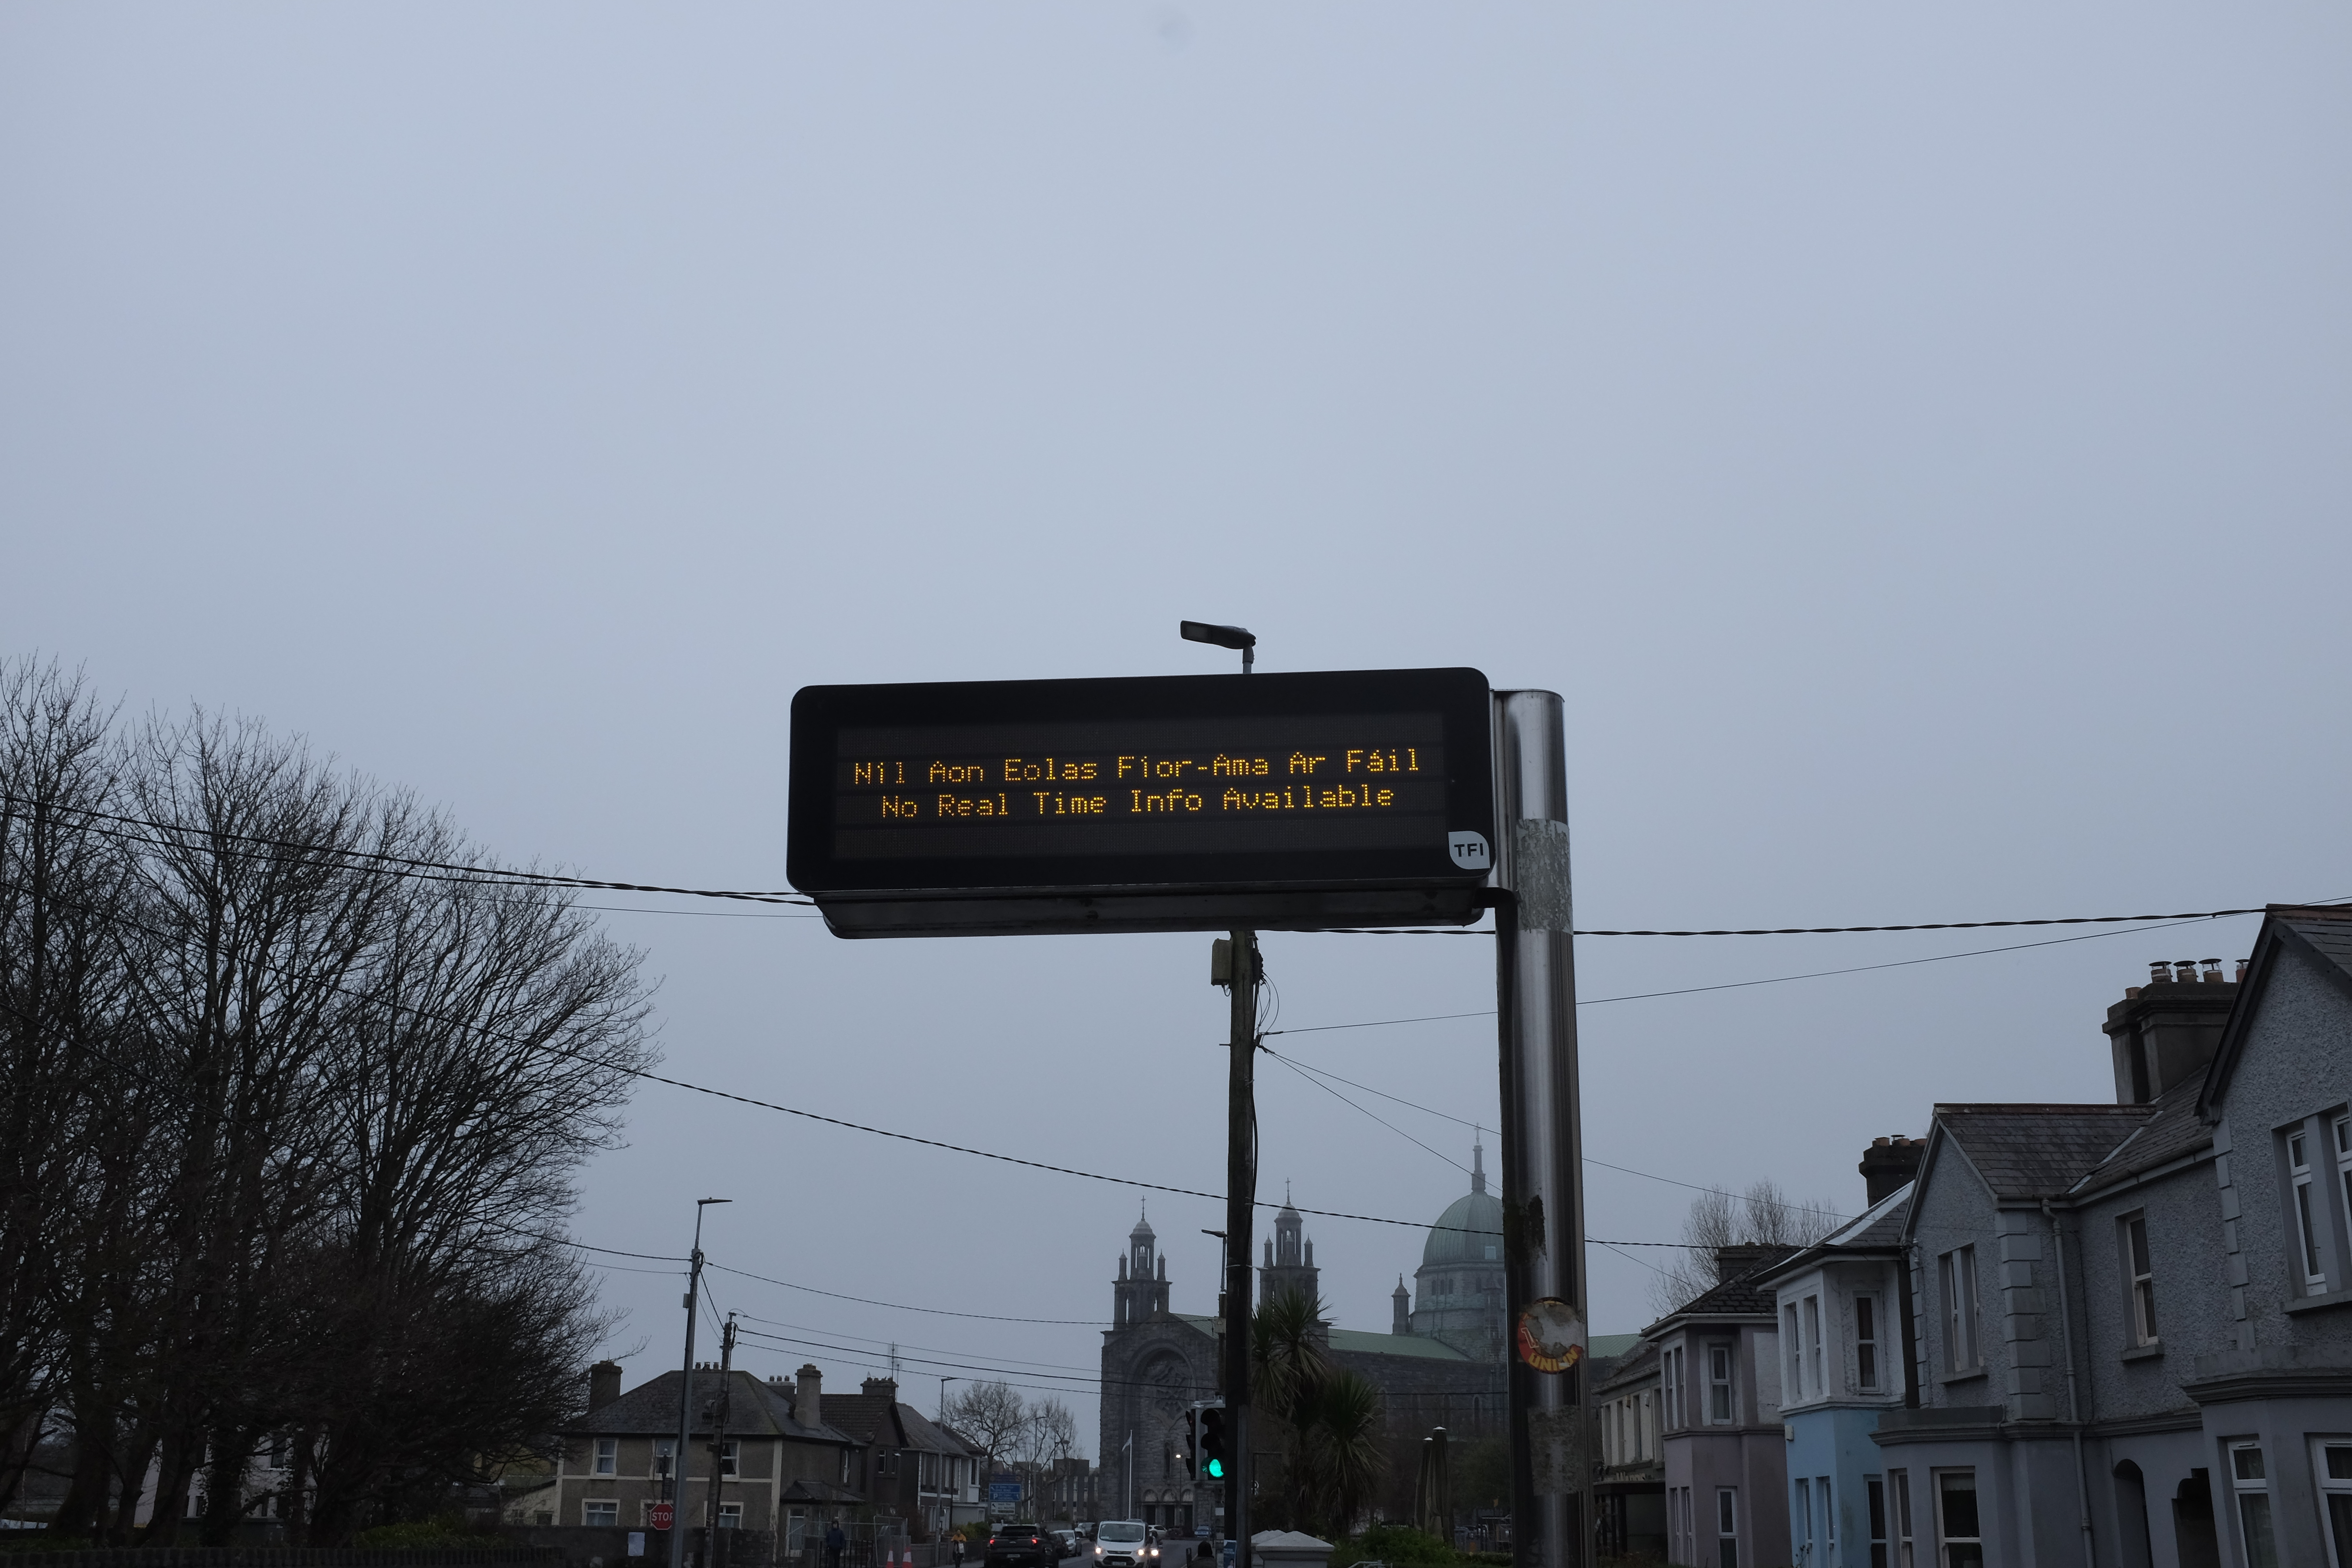
\includegraphics[width=0.8\textwidth]{./images/DSCF3477.JPG}
    \caption{Photograph of a TFI display erroring due to the clocks going forward [Taken: 2025--03--30]}
    \label{fig:tfierror}
\end{figure}

Furthermore, any existing solution that attempts to give public transport users live updates can be unreliable, slow to update, difficult to use, and only supports one type of transport which forces users to download or bookmark numerous different website and apps, and learn the different interfaces \& quirks for each.
Figure~\ref{fig:tfierror} above is a recent example of this: the few bus stops in Galway that actually have a live information display all displayed error messages on Sunday the 30\textsuperscript{th} of March because the clocks went forward by an hour and the system broke.
There is a need for a robust and reliable solution for public transport users who want to know where their service is.
\\\\
With this being said, the main use cases that were kept in mind during the design process were:
\begin{itemize}
    \item   A bus user waiting for their bus that hasn't shown up when it was supposed to and needs to know where it actually is so they can adjust their plans accordingly;
    \item   A train user waiting for their train that hasn't shown up;
    \item   A train user on a train wondering when they will arrive at their destination;
    \item   A Luas user who wants to catch the next Luas from their nearest stop.
\end{itemize}

\section{Constraints}
The primary constraint on this project is the availability of data.
Different public transport providers have different APIs which provide different types of data:
some don't provide location data, others don't provide punctuality data, and others don't have any API at all.
Other constraints include:
\begin{itemize}
    \item   API rate limits \& update frequencies;
    \item   Cost of compute \& storage resources;
    \item   API security policies which limit what kind of requests can be made and from what origin;
    \item   Availability of live data for certain geographical locations.
\end{itemize}

\chapter{Research \& Planning}
\section{Similar Services}
As background research for this project, a list of transport-tracking applications available online was compiled, with each application then being analysed to determine their positive characteristics from which inspiration should be taken and their negative characteristics which should be avoided or fixed.

\subsection{Irish Rail Live Map}
The Irish Rail Live Map\supercite{liveir} displays the current location of Irish Rail intercity, commuter, \& DART services, with clickable icons that display information about the selected service including the lateness of the train and its next stop.
\begin{figure}[H]
    \centering
    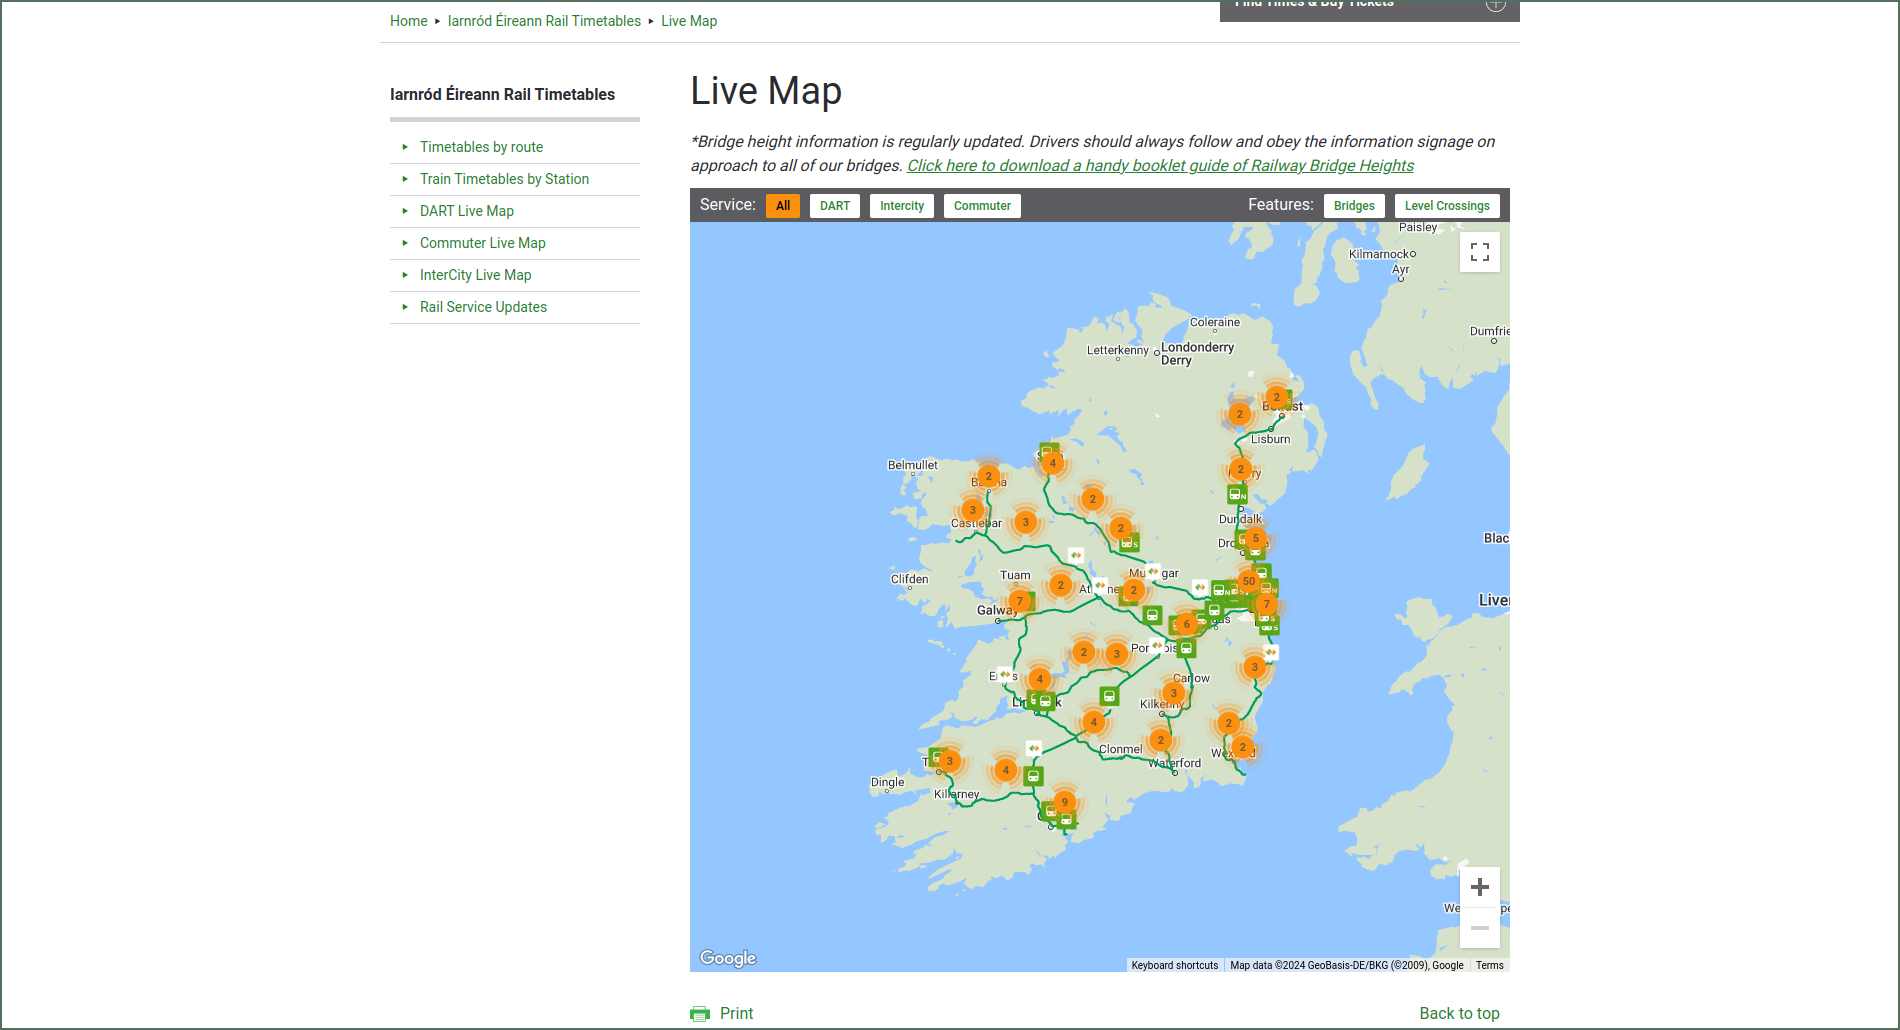
\includegraphics[width=\textwidth]{../PDD/images/irlive.png}
    \caption{Irish Rail live map}
\end{figure}

Strengths of the Irish Rail live map that were identified include:
\begin{itemize}
    \item   Services can be clicked on to display a pop-up panel showing the punctuality of that service, the next stop of that service, and the stops on that service's route;
    \item   There are basic filtering options to display a specific type of service such as DARTs;
    \item   Bridges, level crossings, \& stations are shown on the map.
            The stations can also be selected and information about them viewed.
\end{itemize}

Limitations of the Irish Rail live map that were identified include:
\begin{itemize}
    \item   The pop-up information panel covers the entire map and hides it;
    \item   There is no search feature to find a specific service;
    \item   The filtering options are greatly limited;
    \item   The UI is slow and not particularly responsive;
    \item   There is no visual distinction between the icons for different kinds of services.
\end{itemize}

\subsection{Google Maps}
Google Maps\supercite{gmaps} is a common choice for finding the next the upcoming nearby services and route planning.
It covers a number of different types of service, include buses \& trains.
The mobile UI has been included here alongside the desktop UI as there is no live service information available on the desktop version of Google Maps.

\begin{figure}[H]
    \centering
    \begin{subfigure}[c]{0.2\textwidth}
        \centering
        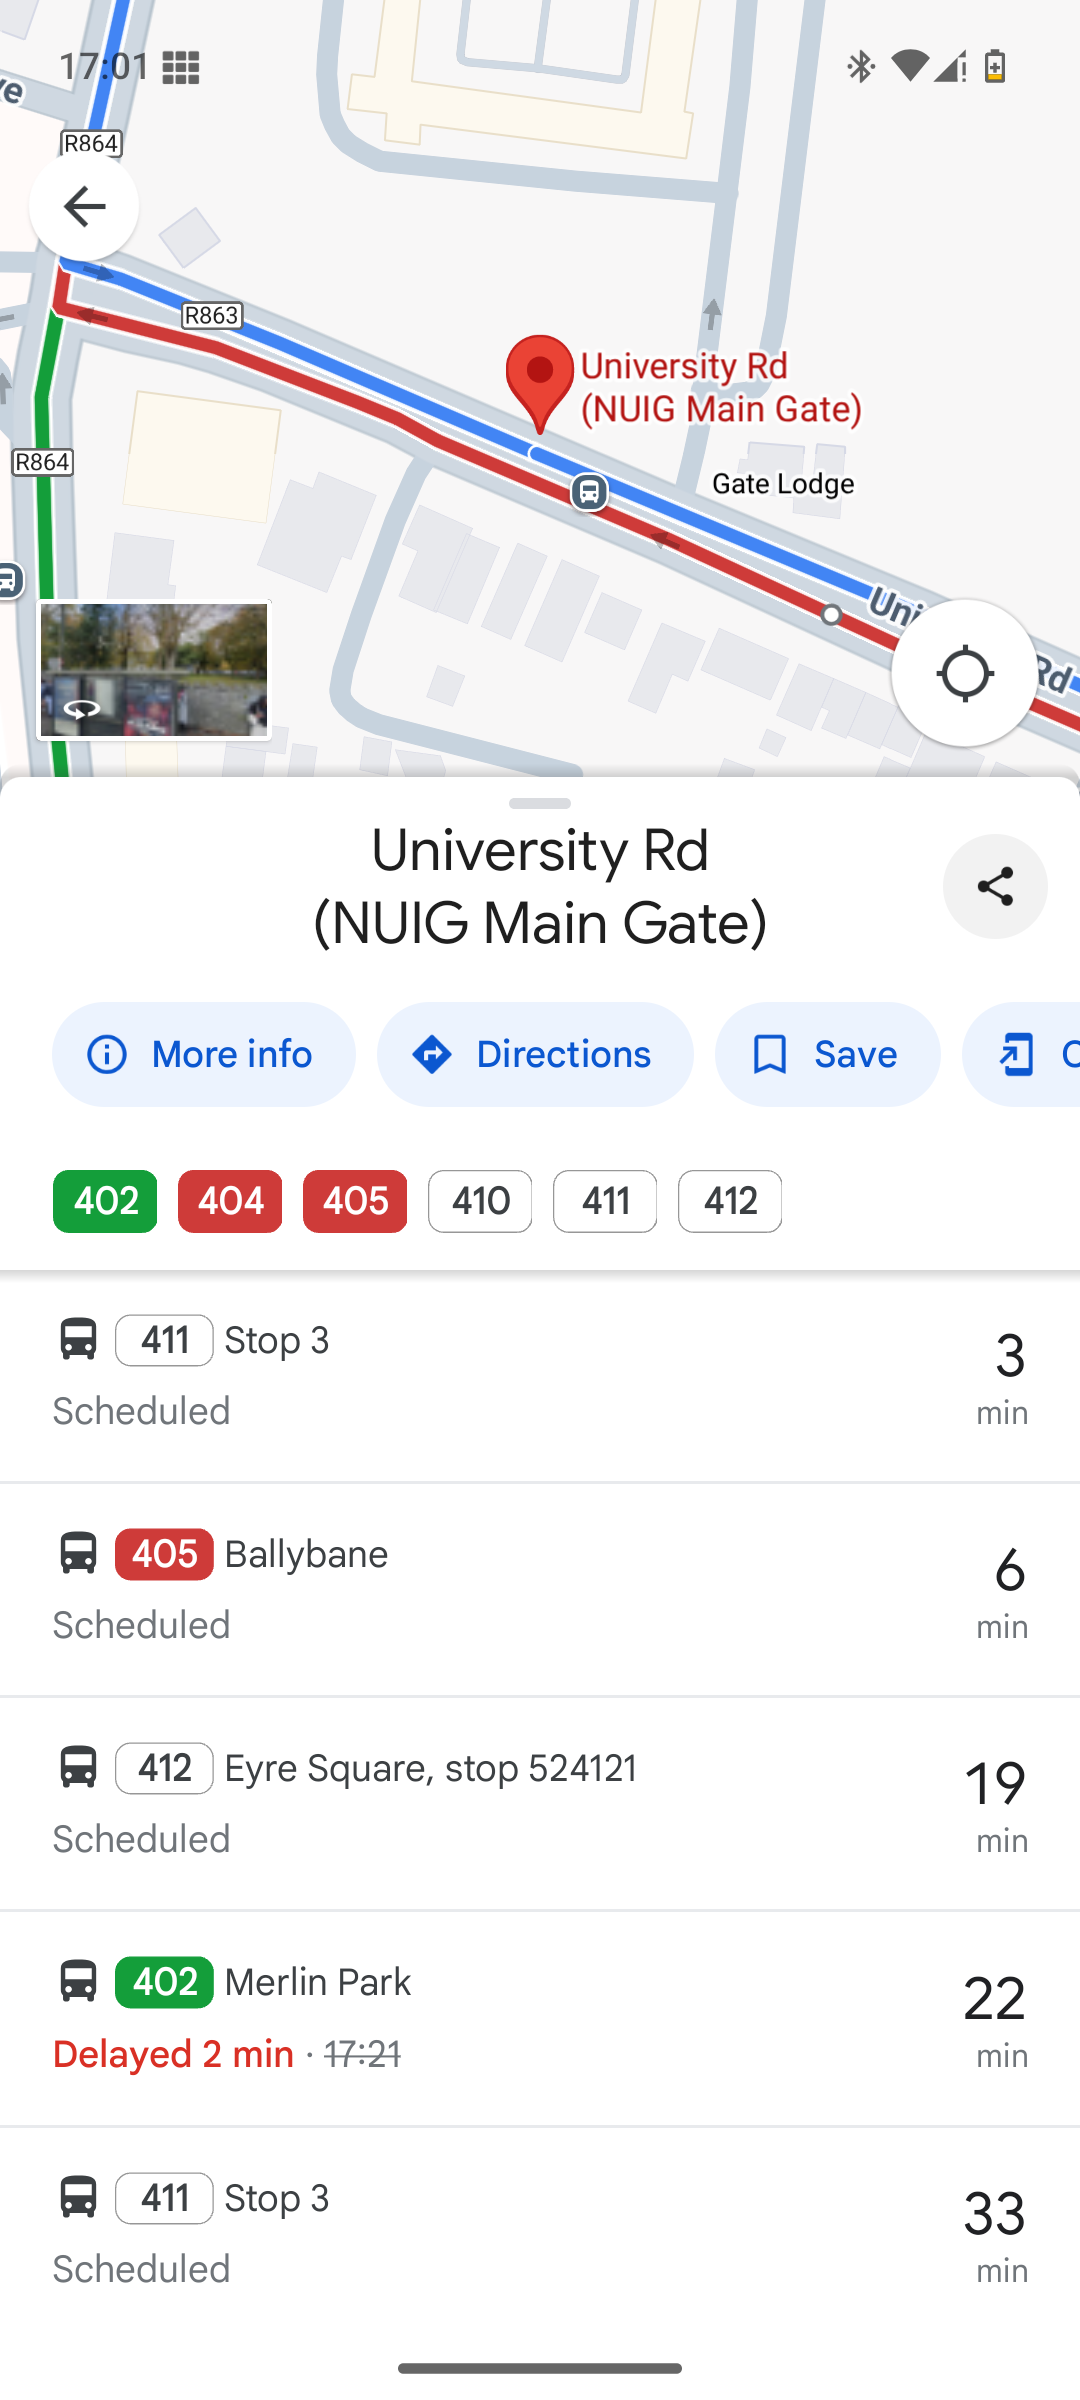
\includegraphics[width=\textwidth]{../PDD/images/gmobile.png}
        \caption{Mobile view}
    \end{subfigure}
    \hfill
    \begin{subfigure}[c]{0.79\textwidth}
        \centering
        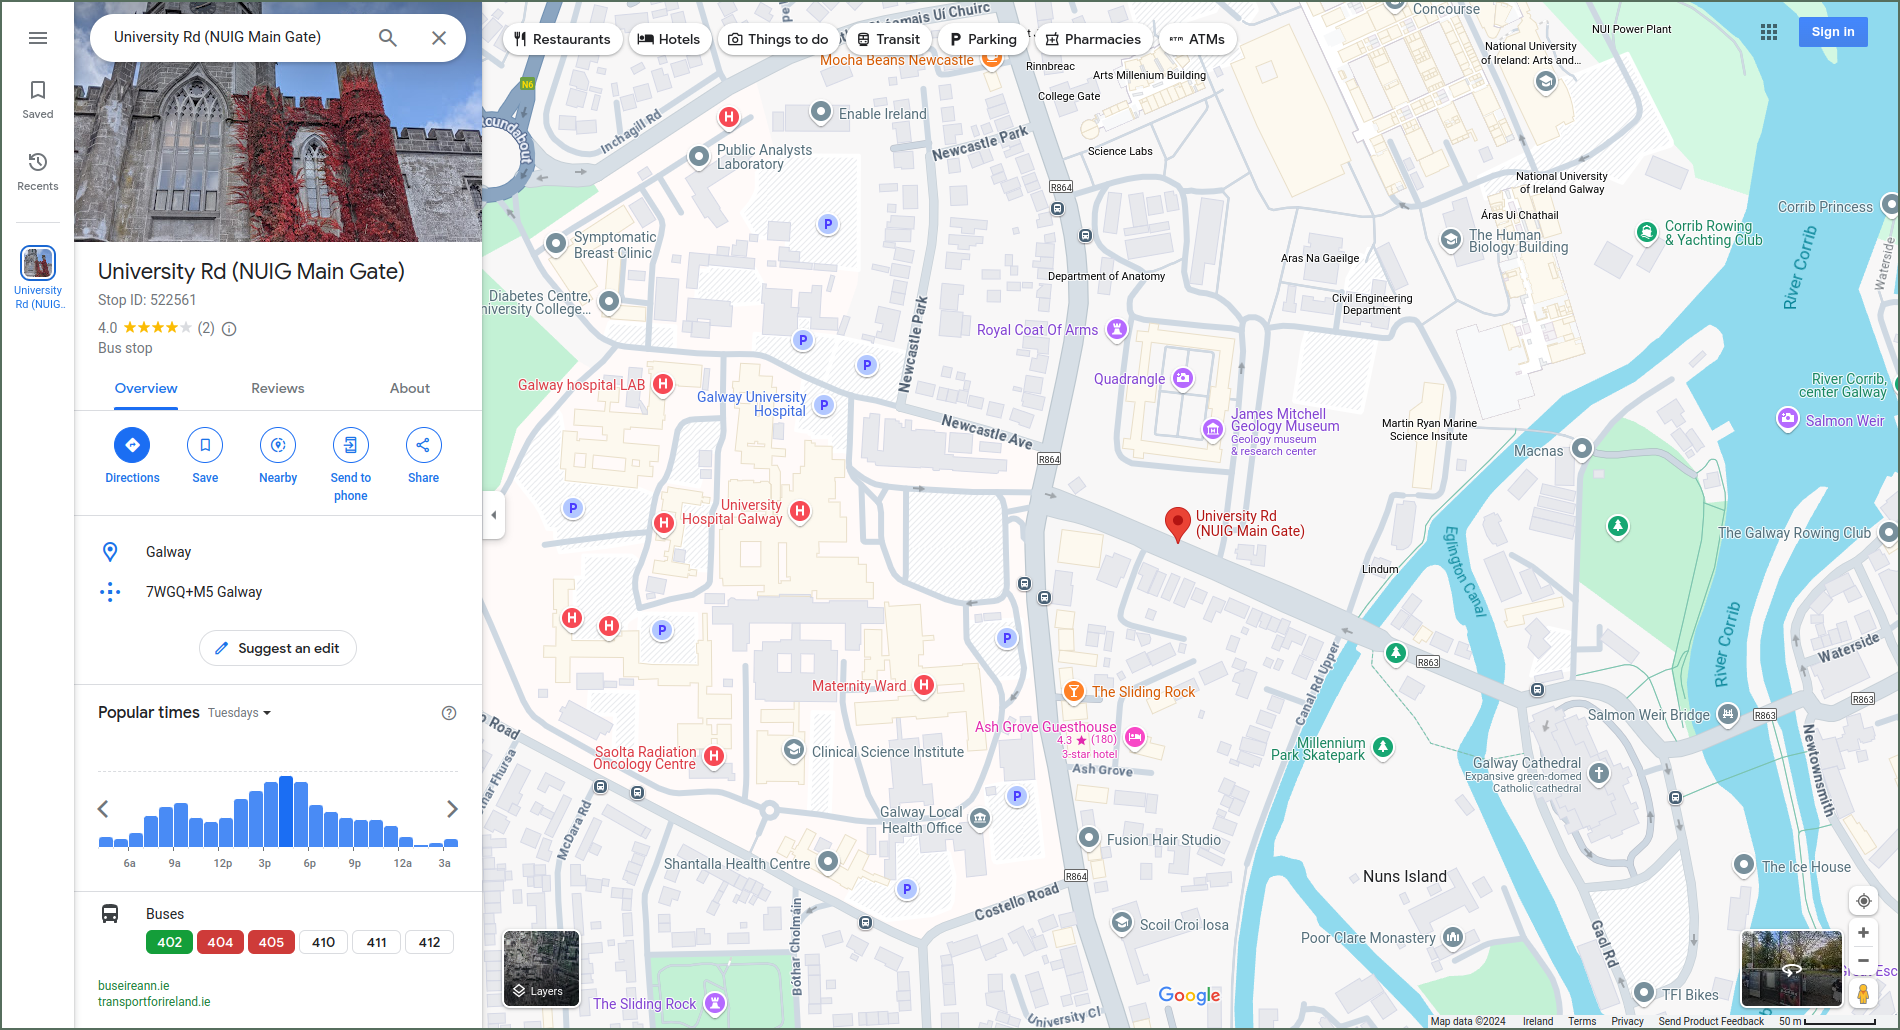
\includegraphics[width=\textwidth]{../PDD/images/gdesk.png}
        \caption{Desktop view}
    \end{subfigure}
    \caption{Google Maps mobile \& desktop views}
\end{figure}

Strengths of Google Maps include:
\begin{itemize}
    \item   It facilitates route determination, and can tell the user about what services they need to take to get any arbitrary location;
    \item   The mobile version lists when services are due and how long they are expected to be delayed.
\end{itemize}

Limitations of Google Maps include:
\begin{itemize}
    \item   There is no live service information on the desktop version;
    \item   Vehicle locations are not plotted on the map and thus the user cannot tell where the service actually is;
    \item   Specific services cannot be searched for, and there is no filtering to display only a certain type of service.
\end{itemize}

\subsection{TFI Live Departures}
The TFI Live Departures map\supercite{tfilive} shows live departure information for both bus stops and train stations.
\begin{figure}[H]
    \centering
    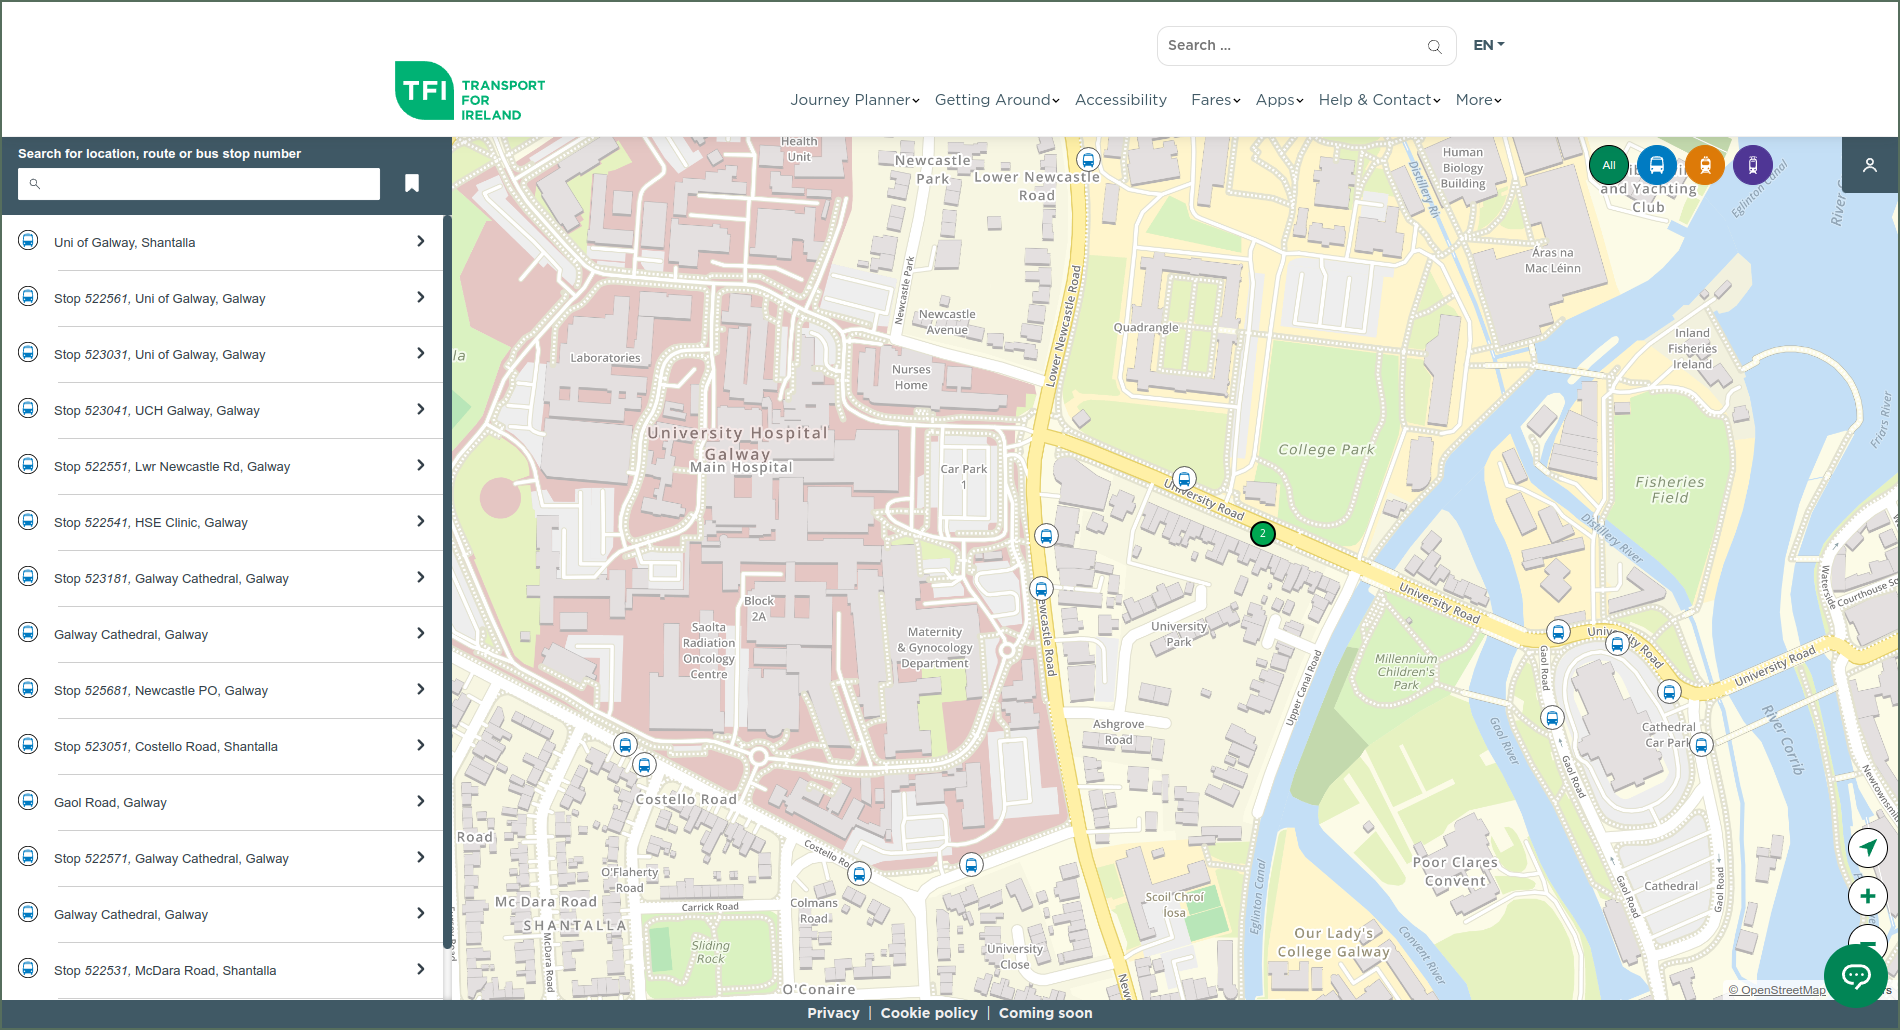
\includegraphics[width=\textwidth]{../PDD/images/tfi.png}
    \caption{TFI Live Departures map}
\end{figure}

Strengths of the TFI Live Departures map include:
\begin{itemize}
    \item   A stop or a station can be clicked on to show a pop-up information panel that appears at the side of the screen and does not cover the map;
    \item   There is a powerful search feature that allows the user to search by location, route, or stop number;
    \item   If a specific route is selected, the route is highlighted on the map and its stops are plotted;
    \item   The map is highly detailed, making it easier to find a particular location on the map and find nearby services.
\end{itemize}

Limitations of the TFI Live Departures map include:
\begin{itemize}
    \item   The map doesn't show the live locations of the services, it shows the stops or stations from which the services depart;
    \item   The map has no filtering options beyond the search feature;
    \item   The map has to be zoomed in very far to actually display the stations in that area, making the map more difficult to use \& navigate;
    \item   It doesn't say whether or not services will be delayed or where they currently are, only saying when they are scheduled for.
\end{itemize}

\subsection{Flightradar24}
Flightradar24\supercite{radar} is a live-tracking application for monitoring aeroplane \& helicopter flights;
while not public transport and therefore not within the scope of this project, this application has nonetheless chosen to be included in this analysis as it is particularly good example of transport-tracking UI, and is highly successful
\begin{figure}[H]
    \centering
    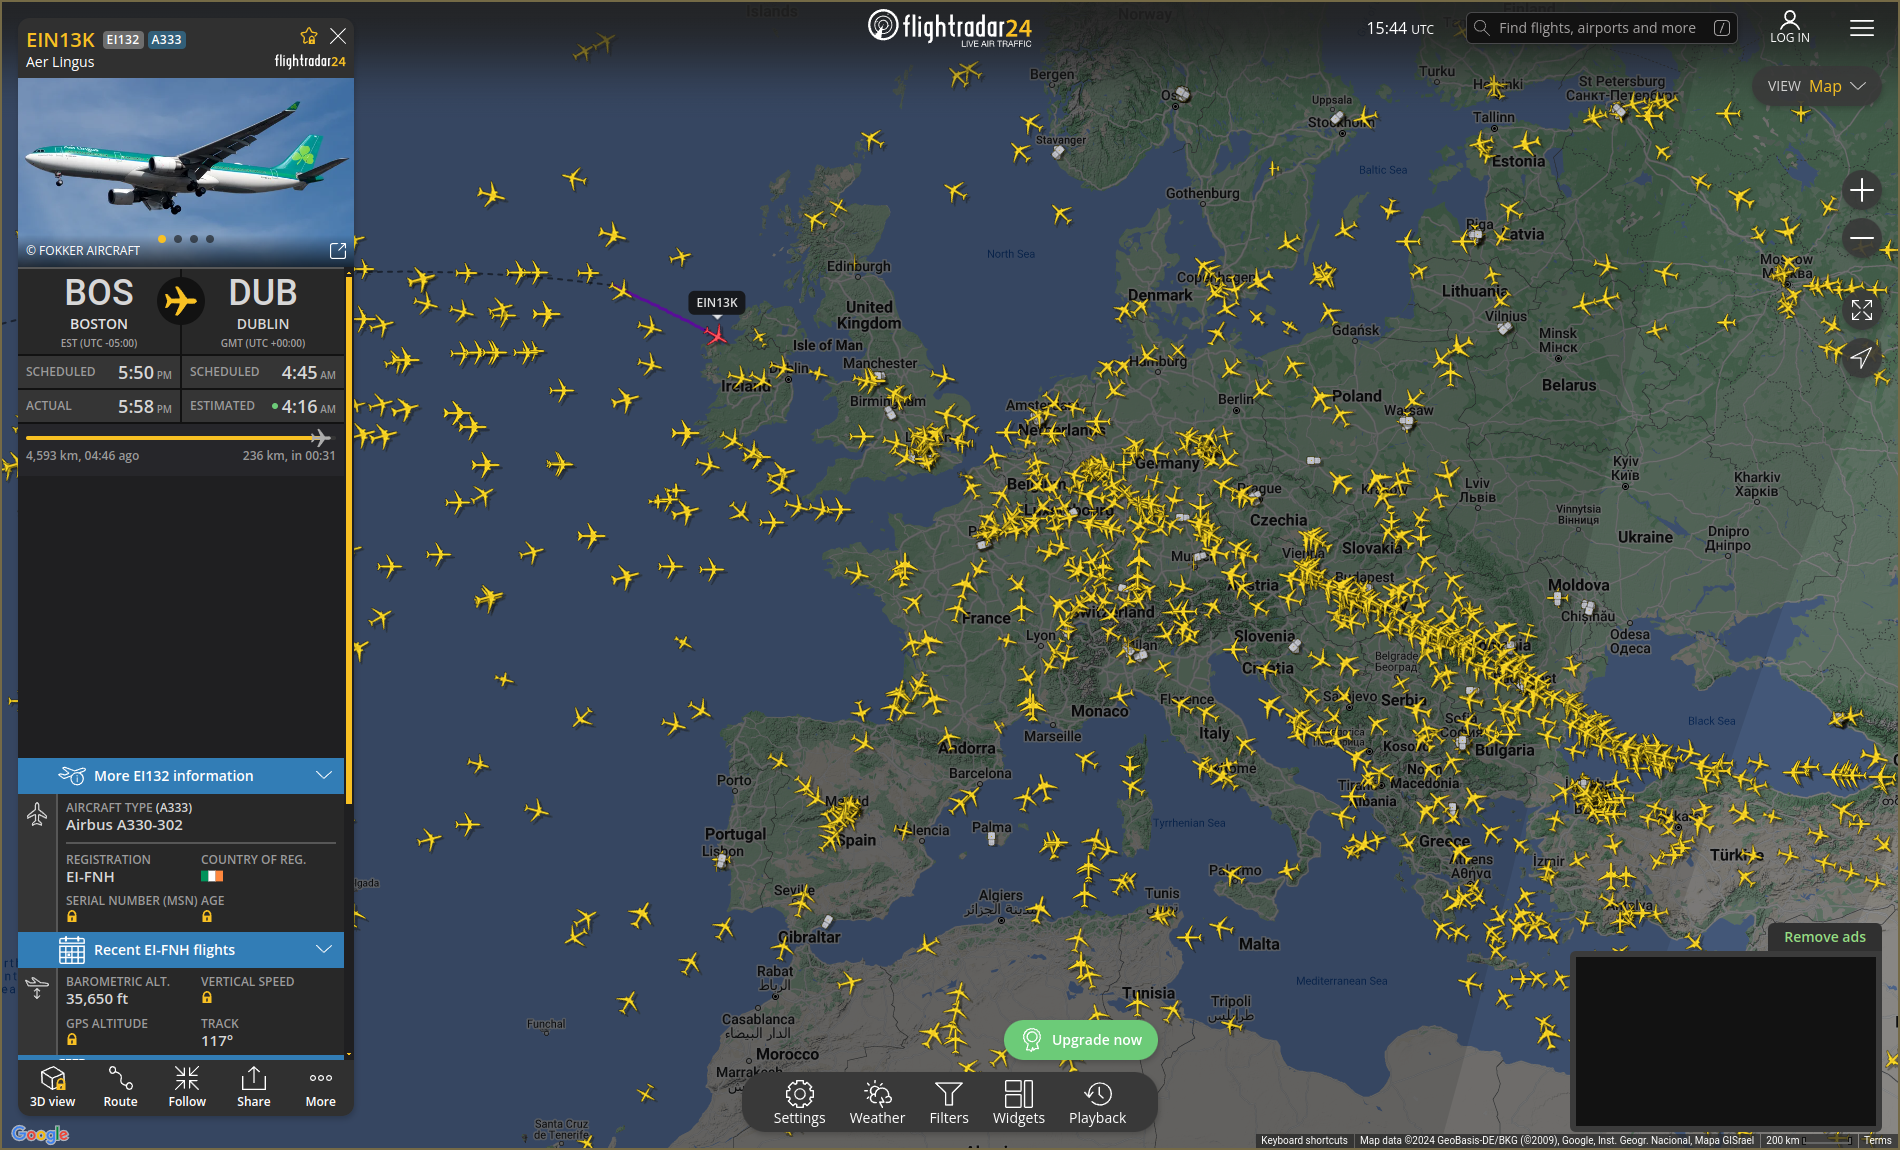
\includegraphics[width=\textwidth]{../PDD/images/flightradar.png}
    \caption{Flightradar24 UI}
\end{figure}

Strengths of Flightradar24 include:
\begin{itemize}
    \item   Ability to select a given service and open a pop-up panel that displays details about that service;
    \item   Selected services are highlighted in red on the map;
    \item   The information panel shows the scheduled departure time, the actual departure time, the scheduled arrival time, \& the estimated arrival time;
    \item   The information panel displays an image of the selected vehicle;
    \item   Searching \& filtering features;
    \item   Larger planes have larger icons on the map and helicopters have distinct icons from planes.
\end{itemize}

Limitations of Flightradar24 include:
\begin{itemize}
    \item   Bookmarking a vehicle requires a paid account;
    \item   The UI contains advertisements for free users.
\end{itemize}

\section{Data Sources}
\subsection{Irish Rail API}
Live train data, including DART information, can be sourced from the Irish Rail Realtime API\supercite{irishrailapi}.
This is a mostly RESTful-like  API which seems to be a legacy hybrid between REST\supercite{fielding2000rest} (Representational State Transfer) and SOAP\supercite{box2000soap} (Simple Object Access Protocol): unlike SOAP, it accepts HTTP \verb|GET| requests instead of a HTTP \verb|POST| of an XML envelope containing the request, but it doesn't use resource-based URLs and returns a namespaced XML response instead of plain XML.
Nonetheless, it can be interacted with in more or less the same way as one would a REST API to obtain data.
It provides a number of endpoints, with the relevant endpoints to this project being:
\begin{itemize}
    \item   \verb|/getAllStationsXML| and \verb|getAllStationsXML_WithStationType?StationType=<A,M,S,D>| which returns information about Irish Rail stations including latitude \& longitude.
    \item   \verb|/getCurrentTrainsXML| and \verb|/getCurrentTrainsXML_WithTrainType?=<A,M,S,D>| which returns information about all the currently running trains (with latitude \& longitude), including trains that are due to depart within 10 minutes of the query time.
    \item   \verb|/getStationDataByCodeXML?StationCode=<station_code>| which returns the trains due to serve the station in question in the next 90 minutes.
\end{itemize}

The documentation page for the API warns that some areas are not fully supported for real-time information due to the central signalling system being subject to ``ongoing work to support this real-time facility'' and that, in the case that a train is in an area of the rail system where real-time data is unavailable, the scheduled data for the train will be returned instead.
The extent to which coverage of real-time data is available today is unclear, as the API documentation page has not been updated since the 8\textsuperscript{th} of December 2015 at the very latest\supercite{irishrail-api-archive} (although a more realistic estimate would be 2011 based off example dates used in the documentation) and so is now likely nearly a decade out-of-date, but this does not affect how the data will have to be processed very much;
since the scheduling information is just returned in the absence of real-time data, this can be treated as a best approximation of the real-time data and does not need to be handled differently.

\subsection{Luas API}
The Luas API\supercite{luasapi} is an XML-over-HTTP API with a REST-like interface that provides real-time updates of expected Luas arrivals for a given Luas stop, based upon the location data of the trams from their Automatic Vehicle Location System (AVLS).
No location data about individual trams is made publicly available;
instead each stop must be queried individually using the \verb|/get.ashx?action=forecast&stop=<stop_code>| endpoint, which returns an XML file with a list of all inbound \& outbound trams due into that stop.

\subsection{NTA GTFS API}
The National Transport Authority (NTA) provides a General Transit Feed Specification (GTFS)\supercite{gtfs} REST API named GTFS-Realtime\supercite{gtfsapi} which provides real-time location data about buses operating in Ireland.
GTFS is a standardised format for public transport schedules \& associated geographic information that provides both static data (such as timetables, routes, \& stop locations) and real-time data (such as live location data).
The static GTFS feed is made up of comma-separated value files (as is standard) and the real-time data is returned in JSON format from the REST API endpoint \verb|gtfsr/v2/Vehicles[?format=json]|.
It is free to use, but requires an API key for access.

\section{Technologies}
\subsection{Backend Technologies}
\subsubsection{Server-Based versus Serverless Architectures}
The first choice to be made for the backend technologies for this project was whether the backend should be designed using a server-based or serverless architecture. 
A traditional server-based model was initially considered, either running on its own dedicated hardware or making use of a Virtual Private Server (VPS)\supercite{AWS:VPS} but was ultimately rejected.
A server-based architecture requires extensive management of infrastructure, including the provisioning of hardware, system administration, and maintenance of the server application itself.
Despite extensive personal experience with Linux-based and UNIX-like operating systems, the ongoing administration of a server would distract from the development of the application itself, and would be very difficult to scale to make the application available to a large number of users.
While scaling issues could be partially mitigated with the utilisation of containerisation and a server-based microservices architecture\supercite{IBM:Microservices, AWS:Microservices} using technologies such as Docker\supercite{DockerEngineDocs}, it would nonetheless take a large amount of administrative effort to scale the application as usage demands grew.
\\\\
In contrast, serverless architectures\supercite{digitalocean_serverless_2023, google_serverless_2025, aws_serverless_2025} abstract away these infrastructure concerns, allowing the focus of the project to be solely on the application logic.
Since serverless functions are invoked on demand and billing for serverless models is based solely upon the usage, serverless architectures are generally much more cost-effective for the workloads with variable or intermittent traffic that would be expected for a user-facing application such as this one.
The serverless model lends itself especially well to a microservices architecture, which allows the system to broken into small, independent services responsible for their own pieces of functionality, with each microservice being independently deployable and scalable.
Instead of establishing or purchasing server infrastructure in advance, a serverless architecture can automatically scale up or down to meet the demand put upon it, preventing outages when large strain is put upon the service and preventing excessive financial or computational costs when there is low usage;
the issue of over-provisioning or under-provisioning of compute resources is entirely circumvented, and the need for load balancers is eliminated entirely.
Serverless functions support event-driven architecture, making them a natural fit for a system that must react to user demands as they occur.
Furthermore, the fast time-to-production of serverless architectures results in faster iteration \& experimentation, easier integration into CI/CD pipelines for continuous delivery, and simplifies rollbacks (should they be necessary) by deploying only small, isolated units, all without the need to spin up servers or configure deployment environment.
\\\\
The ephemeral nature of serverless functions makes them highly fault-tolerant, as an error in a function execution will only affect that execution, whereas an improperly handled error in a server architecture could, in the very worst-case scenario, bring the entire system down and require a reboot.
Moreover, although not especially relevant for this project as it does not handle sensitive data, the attack surface for a serverless architecture is much smaller and there is no need to manually configure server patches or firewall rules, as these are handled by the serverless provider.
For these reasons, a serverless architecture was chosen for this project.

\subsubsection{Serverless Platforms}
A number of serverless platforms were considered for this project, including Amazon Web Services (AWS)\supercite{aws}, Google Cloud\supercite{googlecloud}, Microsoft Azure\supercite{azure}, and Cloudflare\supercite{cloudflare}.
While these platforms have innumerable differences, and are better and worse suited for different applications, a brief overview of their strengths \& weaknesses as considered for this project is as follows:
\begin{itemize}
    \item   AWS has a mature \& extensive ecosystem with broad service integration and a generous free tier, but its complexity can result in a steeper learning curve and a more complex initial set-up.
    \item   Google Cloud has a simpler set-up, and tight integration with Firebase \& Google APIs along with a similarly generous free tier, but fewer advanced features, less control over configuration, and a less extensive ecosystem.
    \item   Microsoft Azure has a deep integration with the Microsoft ecosystem such as SQL server\supercite{azuresql}, but less community support and a steep learning curve for non-Windows developers.
    \item   Cloudflare has extremely low latency, excellent support for edge computing\supercite{ibm_edge_computing} (running on servers geographically close to users), and is great for lightweight apps, but has extremely limited memory and runtime, making it unsuitable for heavy backend logic.
            Its database \& storage solutions are also not as mature or as scalable as comparable solutions.
\end{itemize}

AWS and Google cloud offer the most generous free tiers, while Cloudflare has very tight limits (CPU time is limited to 10ms maximum in the free tier\supercite{cloudflareworkers}) and thus is only suitable for very lightweight tasks, not the kind of extensive data processing that this application will be engaging in.
Therefore, AWS was chosen as the serverless platform for this project as it is was deemed to be the most flexible \& affordable option.

\subsubsection{Relational versus Non-Relational Databases}
AWS offers a wide array of relational and non-relational database services, so the next choice was between a relational \& non-relational database.
\textbf{Relational databases} store data in tables using fixed schemata consisting of rows \& columns, and use SQL for querying;
relationships between tables are strictly enforced with the use of foreign keys.
These rigid, pre-defined schemata are excellent for data integrity \& relational consistency, and are suitable for applications in which relationships between entities are complex and querying across those relationships is common.
\\\\
\textbf{Non-relational databases} store data in more flexible formats, such as key-value pairs, JSON documents, or graphs.
They are more suitable to scaling horizontally and for handling unstructured or semi-structured data.
The simplified structure means that they can be very high performance for simple read/write patterns, and are ideal for applications that handle large volumes of fast-changing or unstructured data.
\\\\
For this application, data is semi-structured and varies greatly by API source.
The data is updated very frequently, which would require many \mintinline{sql}{JOIN} operations or schema migrations for a normalised relational database.
Non-relational databases, on the other hand, offer flexibility for heterogeneous transport data with different attributes, are more suitable for real-time data ingestion \& retrieval due to low-latency reads \& writes, and can support on-demand scaling without the need for the manual intervention required by relational databases to be scaled up;
a non-relational database structure was selected for this reason.
\\\\
AWS offers several non-relational database services, each of which is optimised for a different use case\supercite{awsdatabases}:
\begin{itemize}
    \item   \textbf{Amazon DynamoDB}\supercite{dynamodb} is a fully-managed, serverless No-SQL database designed for low-latency, high-throughput workflows that supports storing data as key-value pair or as JSON-like documents.
            Key features of DynamoDB include the choice between on-demand or provisioned capacity, global tables for replication across multiple geographic regions, and fine-grained access control with Amazon Identity and Access Management (IAM).

    \item   \textbf{Amazon DocumentDB}\supercite{documentdb} is a fully-managed, document-based database using JSON-like BSON with MongoDB compatibilities, designed for applications using MongoDB APIs.
            However, unlike DynamoDB, it is not fully serverless, and is instead a managed cluster-based service that must be provisioned \& scaled manually.

    \item   \textbf{Amazon ElastiCache}\supercite{elasticache} is an in-memory data store for extremely fast caching (sub-millisecond response times) and changing data, with data stored only per session.
            However, it cannot be used for persistent data storage, making it insufficient as a sole database service for this application.

    \item   \textbf{Amazon Neptune}\supercite{neptune} is a managed database for storing \& querying relationships using graph models, generally used for recommendation engines \& knowledge graphs and therefore not suitable for this application.

    \item   \textbf{Amazon Timestream}\supercite{timestream} is a time-series database that is purpose-built for the storage and analysis of time-series data, i.e., timestamped data.
            This would be a good choice for the historical analysis side of this application, but inappropriate for real-time data.

    \item   \textbf{Amazon OpenSearch service}\supercite{opensearch} is a distributed full-text search \& analytics engine based upon Elasticsearch that supports advanced filtering, sorting, \& ranking of query results on an \textit{ad-hoc} basis by default and supports JSON document ingestion.
            However, the higher querying flexibility comes at the cost of higher-latency queries, making it less appropriate for real-time data.
\end{itemize}

DynamoDB was chosen for the database service due to its suitability for the data being processed, its scalability, and its low-latencies.

\subsubsection{Programming Language}
AWS Lambda functions officially support many programming languages, including Node JS, Python, Java, C\#, \& Go;
custom runtime environments can also be created, making practically any language usable within AWS Lambda functions with some effort.
Due to previous experience with these programming languages, the main options considered for this project were Node JS, Python, \& Java:
\begin{itemize}
    \item   Node JS\supercite{node} is a good choice for event-driven \& real-time web applications because of its non-blocking IO, fast cold starts for latency-sensitive functions, and extensive library ecosystem.
            Asynchronous operations are supported out-of-the-box, making it a good choice for querying external APIs.
            However, it can become complex to manage for lengthy source files, and can be cumbersome to write compared to something like Python.
            An advantage of writing the backend in Node JS would be that both the frontend \& the backend would utilise JavaScript code, meaning that the same tooling could be used for both.

    \item   Python\supercite{python} is a good choice for polling of APIs \& data ingestion due to its clean syntax, data parsing features, and extensive library ecosystem.
            Development \& prototyping in Python is fast and easy to manage, but it does not have built-in support for asynchronous programming.
            Python is generally slightly slower than Node JS, and start-up time for Python Lambda functions can be longer.

    \item   Java\supercite{java} is a good choice for complex, enterprise-grade applications due to its strong typing \& compile-time safety, and has a mature library ecosystem.
            However, it can be slower to write due to its verbose syntax, and development environments can be more complex to set up \& configure.
            Despite having fast execution times, it can be slow to start up for Lambda functions as the JVM must be initialised each time, leading to $\sim$1--2 seconds of delay.
\end{itemize}

Java was rejected on the basis that its slow start-up times made it unsuitable for this application, so the decision came down to whether the speed of execution for Node JS or the speed of development for Python should be favoured;
ultimately, it was decided that Python would be a better choice for rapid prototyping \& development, as the execution speed differences between the two languages are negligible (in this scenario), but the development speed differences are not.

\subsection{Frontend Technologies}
\subsubsection{JavaScript Frameworks}
While a web application like this could be developed using HTML and JavaScript alone, the complexity \& dynamic nature of the application means that a JavaScript framework would more suitable for the benefits of re-usability \& modularity, simplified application state management, optimised performance, and extensive library ecosystems.
The main frameworks considered were React, Angular, \& Vue due to their widespread popularity, good documentation, and extensive feature set:
\begin{itemize}
    \item   \textbf{React}\supercite{react} is the most popular choice of the three, with a large user community and a wide array of third-party libraries.
        It is component-based, making code easily re-usable and allowing the frontend design to be flexible for different design patterns \& architectures.
        However, it can have a steep learning curve and can be needlessly complicated for simple applications.
        Technically speaking, it is not a full JavaScript framework, as it only provides built-in features for building UI components: it doesn't have built-in features for routing, data fetching, or tight integration with any backend services, although these can be added either with third-party libraries or by writing custom JavaScript code.
        \\\\
        There is also a mobile development framework built on top of React called \textbf{React Native}\supercite{native}, which allows for native Android \& iOS mobile application to be developed using JavaScript and React components.
        Instead of rendering to a DOM like vanilla React, React Native maps its UI components to native iOS/Android views (i.e., a button in React Native would use the operating system's native button component instead of being defined in HTML).
        This means that the same React Native codebase can be used to write an iOS and an Android application, and means that the performance will be superior to that of a webview application because of the utilisation of native components.
        However, React Native does not support any HTML or CSS, meaning that while a React web application is highly portable to React Native, it is not a simple drop-in solution, and a React web application would have to undergo extensive re-writing to use React Native.

    \item   \textbf{Angular}\supercite{angular} is a complete JavaScript framework for large-scale enterprise applications that comes with complete routing, state management, and a HTTP client out-of-the-box, therefore eliminating much of the need for third-party libraries.
            However, it has a rather steep learning curve, and takes a lot more development time to get up and running than other comparable JavaScript frameworks.
            It requires a lot of boilerplate code and complex configuration, with relatively simple features sometimes taking a great deal of set-up.
            It also rigidly enforces certain best practices, which is both a positive and a negative, as this ties the development into the Angular way of doing things.

    \item   \textbf{Vue}\supercite{vue} is a JavaScript framework known for its simplicity and ease-of-use, with very beginner-friendly syntax that is highly similar in appearance to standard HTML \& JavaScript.
            Reactivity is baked into the framework, with the view updating automatically as data changes, reducing the need to manually update data values.
            All the HTML, CSS, \& JavaScript for a Vue component is contained within a single component file, simplifying development.
            However, it has a far less mature library ecosystem than the other two discussed frameworks, and fragmentation between the Vue 2 version and the Vue 3 version means that the few plug-ins that do exist may not be compatible with the version used.
            Vue's automatic handling of reactivity, while simplifying development, can be a black box that is difficult to understand for debugging purposes.
\end{itemize}

It was decided that React would be the most suitable JavaScript framework for this project, as it has extensive library support, is flexible \& lightweight, and it lends itself to porting the codebase to a native application if so desired in the future.
Since the consideration of native applications is only a secondary objective of this project, the decision was made to focus only on React development and to make use of React-only functionality wherever suitable (such as using HTML + CSS), but to write the components in a clean \& modularised fashion so that a React Native port would not be excessively difficult.

\subsubsection{CSS Frameworks}
A \textbf{CSS framework} is a collection of pre-written styles, utility classes, or components that can be used to help build UIs quickly without reinventing basic functionality.
CSS frameworks allow applications to be responsive by default on mobile devices, and maintain consistency throughout the application.
The two CSS frameworks considered for this application were Tailwind CSS and Bootstrap CSS:
\begin{itemize}
    \item   \textbf{Tailwind CSS}\supercite{tailwind} is a utility-first CSS framework in which the user interface is built by composing utility classes directly in HTML / React code;
            in this context, ``utility first'' refers to the fact that Tailwind does not provide any pre-built components, but instead provides pre-defined utility classes.
            Layout and styling are all done in-line via class names.
            This utility-based approach makes the framework very flexible \& customisable, but comes at the cost of not providing any out-of-the-box re-usable components and require for components to be designed from scratch instead.

    \item   \textbf{Bootstrap CSS}\supercite{bootstrap} is a component-first CSS framework designed to help developers build responsive, styled UIs quickly. 
            It comes with many pre-built components such as buttons and navigation bars, and JavaScript plug-ins for drop-down menus and image carousels.
            This makes it very useful for fast prototyping and building of UIs, but can look generic due to its pre-built components and overriding the default component styles can be time-consuming.
\end{itemize}

Tailwind CSS was chosen for this project due to its flexibility \& customisability, and because its utility-first approach means it integrates very well with React's component-based approach as a component's style can be contained entirely within that component.


\section{Project Management}
\textbf{Agile methodologies}\supercite{agile} were employed throughout this project to facilitate iterative development with continuous feedback \& adaptation:
Agile is a development approach which divides work into phases, emphasising continuous delivery \& improvement.
Tasks are prioritised according to importance \& dependencies, and are approached in a flexible manner so that approaches could be adjusted if something isn't working as intended.
Progress was reflected upon regularly, with areas for improvement being identified and plans adjusted accordingly.
Automated CI/CD pipelines were employed to streamline development, and to ensure that new changes never broke existing functionality.
Progress was tracked in a Markdown diary file, and a physical Kanban\supercite{kanban} board with Post-It notes was used to track planned work, in progress work, \& completed work.
\\\\
The principles of \textbf{clean coding}\supercite{martin2008cleancode} (famously put forward by Robert ``Uncle Bob'' Martin) were also employed to ensure that all code written was easy to read, understand, \& maintain.
Key principles of clean coding involve ensuring that the code is readable with meaningful function \& variable names, ensuring that the code is simple \& concise with each function doing one thing only and doing that thing well, using consistent naming conventions, and employing the Don't Repeat Yourself (DRY) principle which involves the avoidance of duplicated code by creating re-usable functions \& modules.
Code should be structured in a way that is meaningful, and should have proper comments \& documentation where necessary;
comments should only explain \textit{why} something is done, not \textit{what} it does as properly written clean code should be self-explanatory.
Code should also be written in a way that lends itself easily to unit testing, and should be refactored to make testing as simple as possible rather than making the tests more complicated;
if the code is decomposed into functions properly, it should be easier to test, upgrade, \& maintain.
\\\\
Proper functional decomposition also results in code that is less tightly coupled in to specific libraries, platforms, or services, making it more flexible \& easier to port to different services if needs be.
With proper separation of concerns, each function has a single responsibility and so dependencies can be isolated, and abstraction layers can prevent direct dependency on a specific implementation;
if a function is abstracted properly switching libraries or services requires fewer changes and in fewer places.
Isolated functions are also easier to test with mock functions, reducing reliance on real services during unit testing.

\subsection{Version Control}
Any software development project of substantial size should make use of version control software, and Git\supercite{git} was chosen for this project due to its ubiquitousness and extensive personal experience with the software.
GitHub\supercite{github} was chosen as the hosting platform for the Git repository, again largely due to its ubiquitousness and extensive personal experience, but also because of its excellent support for CI/CD operations with GitHub Actions\supercite{githubactions}.
The decision was made to keep all relevant files for this project, including frontend code, backend code, and document files in a single monolithic repository (monorepo) for ease of organisation, a simplified development workflow, and easier CI/CD set-up.
While this is not always advisable for very large projects where multiple teams are collaborating, or projects in which the backend and frontend are truly independent of one another and are developed separately, this works well for projects like this one where development is done by a single individual or a small team\supercite{brito2018monorepos}, and is even used on very large projects where unified versioning and simplified dependency management are of paramount importance, such as at Google\supercite{potvin2016google}.
\\\\
Commits to this repository were made in adherence with the philosophy of \textit{atomic commits}, meaning that each commit represents a single, logical change:
commits are kept as small as reasonably possible, and are made very frequently.
This makes the Git history easier to read, understand, \& revert if needed, makes debugging easier, keeps changes isolated and understandable, and reduces merge conflicts.
This is the generally accepted best practice, as bundling unrelated changes into a single commit can make review, reversion, \& integration of these commits much more difficult\supercite{dias2015untangling}.
\\\\
Meaningful commit messages are of great importance when using version control software, and even more so when making atomic commits as there will be a very large volume of commits \& commit messages.
For this reason, a custom scoped commit message convention was chosen, where each commit message follows the format \verb|[scope]: Details of commit|, where the \verb|scope| can be \verb|[frontend]| for changes to frontend code, \verb|[backend]| for backend code, \verb|[report]| for changes to the {\LaTeX} project report files, and so on.
This ensure consistency \& clarity in commit messages, and the strict formatting of the messages make it easy to parse commit messages in a script should that be necessary.
Recent examples of commit messages to the GitHub repository can be seen in Figure~\ref{fig:reposs} below.

\begin{figure}[H]
    \centering
    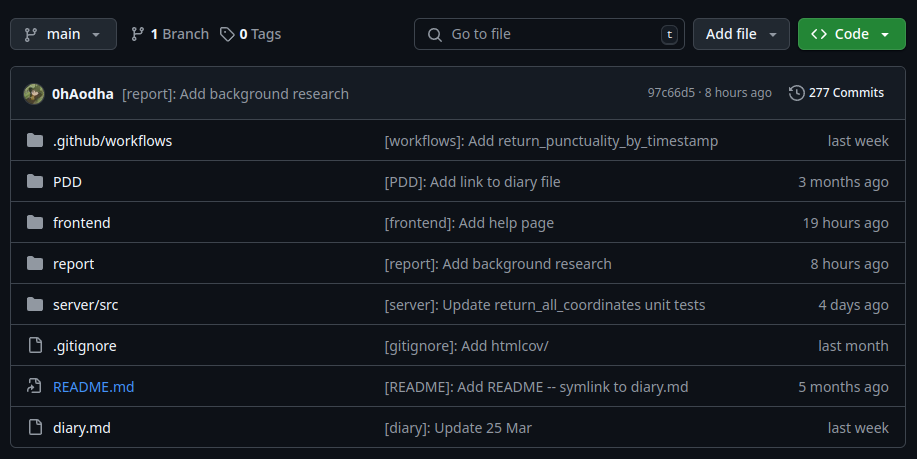
\includegraphics[width=\textwidth]{./images/reposs.png}
    \caption{Screenshot of the repository files on GitHub}
    \label{fig:reposs}
\end{figure}

\chapter{Backend Design \& Implementation}
\begin{figure}[H]
    \centering
    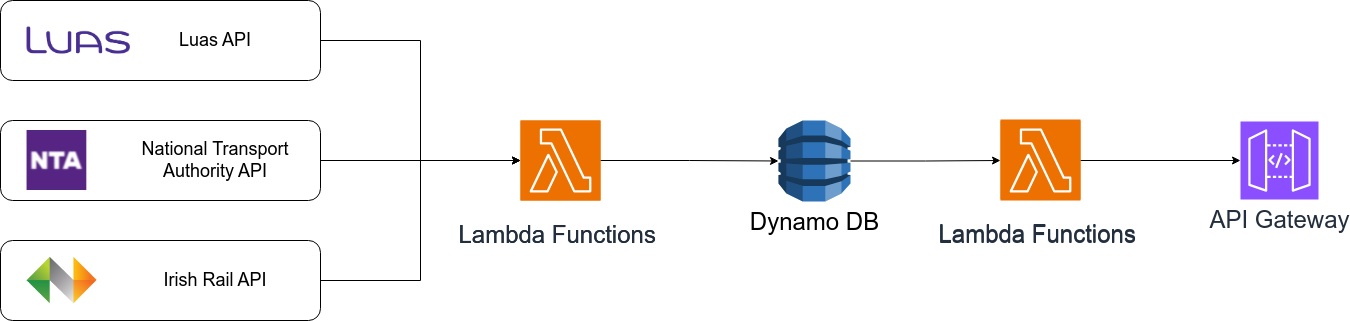
\includegraphics[width=\textwidth]{./images/overall_backend.png}
    \caption{High-level backend architecture}
\end{figure}

\section{Database Design}
Since the chosen database system was DynamoDB, a No-SQL database, the question of how best to separate the data is more open-ended: unlike a relational database, there is no provably correct, optimised structure of separated tables upon which to base the database design.
The decision was made that data would be separated into tables according to the type of data, how its used, and how its updated, thus allowing separation of concerns for functions which update the data and allowing different primary keys and indices to be used for different querying patterns.

\subsubsection{Permanent Data Table}
The permanent data table holds the application data which is unchanging and needs to be updated only rarely, if ever.
This includes information about bus stops, train stations, Luas stops, and bus routes.
This data does not need to be updated regularly, just on an as-needed basis.
Since this data is not temporal in nature, no timestamping of records is necessary.

\begin{code}
\begin{minted}[linenos, breaklines, frame=single]{json}
[
  {
    "objectID": "IrishRailStation-GALWY",
    "objectType": "IrishRailStation",
    "trainStationCode": "GALWY",
    "trainStationID": "170",
    "trainStationAlias": null,
    "trainStationDesc": "Galway",
    "latitude": "53.2736"
    "longitude": "-9.04696",
  },
  {
    "objectID": "BusStop-8460B5226101",
    "objectType": "BusStop",
    "busStopID": "8460B5226101",
    "busStopCode": "522611",
    "busStopName": "Eyre Square",
    "latitude": "53.2750947795551"
    "longitude": "-9.04963289544644",
  },
  {
    "objectID": "BusRoute-4520_67654",
    "objectType": "BusRoute",
    "busRouteID": "4520_67654"
    "busRouteAgencyName": "City Direct",
    "busRouteAgencyID": "7778028",
    "busRouteShortName": "411",
    "busRouteLongName": "Mount Prospect - Eyre Square",
  },
  {
    "objectType": "LuasStop",
    "objectID": "LuasStop-STS",
    "luasStopCode": "STS"
    "luasStopID": "24",
    "luasStopName": "St. Stephen's Green",
    "luasStopIrishName": "Faiche Stiabhna",
    "luasStopIsParkAndRide": "0",
    "luasStopIsCycleAndRide": "0",
    "luasStopLineID": "2",
    "luasStopZoneCountA": "1",
    "luasStopZoneCountB": "1",
    "luasStopSortOrder": "10",
    "luasStopIsEnabled": "1",
    "latitude": "53.3390722222222",
    "longitude": "-6.26133333333333",
  }
]
\end{minted}
\caption{Sample of the various types of items stored in the permanent data table}
\label{listing:permanent_data}
\end{code}

As can be seen in Listing~\ref{listing:permanent_data}, two additional fields are included for each item beyond what is returned for that item by its source API:
the \verb|objectType| to allow for querying based on this attribute and the \verb|objectID|, an attribute constructed from an item's \verb|objectType| and the unique identifier for that item in the system from which it was sourced, thus creating a globally unique identifier for the item.
However (for reasons that will be discussed shortly), this attribute is \textit{not} used as the primary key for the table;
instead, it exists primarily so that each item has a unique identifier that does not need to be constructed on the fly on the frontend, thus allowing the frontend to treat specific items in specific ways.
An example of a use for this is the ``favourites'' functionality: a unique identifier must be saved for each item that is added to a user's favourites.
Defining this unique identifier in the backend rather than the frontend reduces frontend overhead (important when dealing with tens of thousands of items) and also makes the system more flexible.
While the ``favourites'' functionality is implemented fully on the frontend at present, the existence of unique identifiers for items within the table means that this functionality could be transferred to the backend without major re-structuring of the database.
\\\\
There are two ways in which a primary key can be created for a DynamoDB table\supercite{choosing-the-right-key}:
\begin{itemize}
    \item   A simple primary key, consisting solely of a \textbf{partition key}: the attribute which uniquely identifies an item, analogous to simple primary keys in relational database systems.

    \item   A composite primary key, consisting of a partition key and a \textbf{sort key}, analogous to composite primary keys in relational database systems.
            Here, the partition key determines the partition in which an item's data is stored, and the sort key is used to organise the data within that partition.
\end{itemize}

While the \verb|objectID| could be used as a partition key and thus a simple primary key, it was decided not to use the attribute for this purpose as it was not the most efficient option.
The primary function of the permanent data table is to provide data for a user when they want to display a certain type of object, such as bus stops, train stations, Luas stops, or some combination of the three.
Therefore, the most common type of query that the table will be dealing with is queries which seek to return all items of a certain \verb|objectType|.
Partitioning the table by \verb|objectID| would make querying by \verb|objectID| efficient, but all other queries inefficient, and querying by \verb|objectID| is not useful for this application.
Instead, the permanent data table uses a composite primary key, using the \verb|objectType| as the partition key and the \verb|objectID| as the sort key.
Thus, it is very efficient to query by \verb|objectType| and return, for example, all the bus stops and Luas stops in the country.
\\\\
Technically speaking, there is some redundant data in each primary by using the \verb|objectID| as the sort key when the partition key is the \verb|objectType|: since the \verb|objectID| already contains the \verb|objectType|, it is repeated.
However, the unique identifier for each item is different depending on the system from which it was sourced:
for train stations, the unique identifier is named \verb|trainStationCode|, while the unique identifier for bus stops is named \verb|busStopID|.
To use these fields as sort key, they would have to be renamed in each item to some identical title, thus adding overhead to the process of fetching data, and making the table less human-readable.
Since the \verb|objectID| was to be constructed regardless for use on the frontend, it is therefore more efficient to re-use it as the sort key, even if it does result in a few bytes of duplicated data in the primary key of each item.

% The primary key of this table is the \verb|objectID|, necessarily unique to each record in the table.
% This is constructed as a combination of the \verb|objectType| (e.g., \verb|BusStop|, \verb|IrishRailStation|) and the unique identifier for that object returned by the API from which the data was retrieved.
% The prefix of the \verb|objectType| is used here to guarantee uniqueness of the primary key in the case that two objects in the table of differing types have the same ID given to them by their respective source APIs.
% \\\\
% There are two ways in which a primary key can be created for a DynamoDB table\supercite{choosing-the-right-key}:
% \begin{itemize}
%     \item   A simple primary key, consisting solely of a \textbf{partition key}: the attribute which uniquely identifies an item, analogous to simple primary keys in relational database systems.
%
%     \item   A composite primary key, consisting of a partition key and a \textbf{sort key}, analogous to composite primary keys in relational database systems.
%             Here, the partition key determines the partition in which an item's data is stored, and the sort key is used to organise the data within that partition.
% \end{itemize}
%
% Instead of constructing a new attribute \verb|objectID| for an item, it would also be possible to avoid creating a new attribute by instead using a composite primary key, with the partition key being the item's unique identifier in the system from which it came and the sort key being the \verb|objectType|.
% This was rejected in favour of constructing a new attribute, \verb|objectID| to serve as the simple primary key for this table for a number of reasons:
% \begin{itemize}
%     \item   The uniquely identifying attribute for each item given to it by the API from which said item was sourced has a different attribute name for every API;
%             the unique identifier for bus stops is \verb|busStopID|, for train stations is \verb|trainStationCode|, et cetera.
%             To use these values as the primary key in the table, each of these attributes would have to be re-named to some single, unifying title, creating additional parsing overhead when the data is being uploaded to the table, and making the item information more difficult to read for humans.
%
%     \item   Having a single uniquely identifying attribute for each item is useful on the frontend, allowing items to be easily uniquely identified without additional processing, useful for user functionality such as adding an item to the user's ``favourites''.
%
%     \item   The query efficiency improvements typically associated with a DynamoDB composite key would not apply to the type of queries this table is designed for with such a composite key structure.
%             The data from this table will most often be queried by \verb|objectType| in this application, such as in the event that a user wants to see bus stops or train stations or both on a map.
%             The composite key would only speed up querying in the event that, for a number of different items with the same unique identifier, a query was ran on based on the type of those objects sharing an identifier, which is not a situation that is likely to arise for this application.
% \end{itemize}
%
% As mentioned in the final bullet-point above, this table is only intended for a single type of query:
% queries which seek to return all the items in the table of a certain \verb|objectType| or \verb|objectType|s, such as when a frontend user requests to see bus stops, or train stations, or Luas stops, or some combination of the three.
% Therefore, it is imperative that such queries are efficient \& fast. 
% Since we cannot partition the data 

\subsubsection{Transient Data Table}
The transient data table holds the live tracking data for each currently running public transport vehicle in the country, including information about the vehicle and its location.
Similar to the permanent data table, a unique \verb|objectID| is constructed for each item.
A sample of the data stored in the transient data table can be seen below in Listing~\ref{listing:transient_data}:

\begin{code}
\begin{minted}[linenos, breaklines, frame=single]{json}
[
  {
    "objectType": "IrishRailTrain",
    "latenessMessage": "On time",
    "timestamp": "1742897696",
    "trainDirection": "Southbound",
    "trainStatus": "R",
    "trainDetails": "09:41 - Maynooth to Grand Canal Dock ",
    "trainType": "S",
    "objectID": "IrishRailTrain-P656",
    "averagePunctuality": "0",
    "trainUpdate": "Departed Pelletstown next stop Broombridge",
    "trainStatusFull": "Running",
    "longitude": "-6.31388",
    "trainPublicMessage": "P656\\n09:41 - Maynooth to Grand Canal Dock (0 mins late)\\nDeparted Pelletstown next stop Broombridge",
    "trainPunctuality": "0",
    "trainPunctualityStatus": "on-time",
    "trainTypeFull": "Suburban",
    "trainDate": "25 Mar 2025",
    "latitude": "53.3752",
    "trainCode": "P656"
  },
  {
    "objectType": "Bus",
    "busScheduleRelationship": "SCHEDULED",
    "timestamp": "1742908007",
    "busID": "V598",
    "busRoute": "4538_90219",
    "busRouteAgencyName": "Bus Éireann",
    "objectID": "Bus-V598",
    "busRouteLongName": "Galway Bus Station - Derry (Magee Campus Strand Road)",
    "longitude": "-8.50166607",
    "busDirection": "1",
    "busStartDate": "20250325",
    "busRouteShortName": "64",
    "latitude": "54.2190742",
    "busTripID": "4538_114801",
    "busStartTime": "10:30:00"
  },
\end{minted}
\caption{Sample of the various types of items stored in the transient data table}
\label{listing:transient_data}
\end{code}

There are only two types of objects stored in the transient data table: Irish Rail Trains and Buses.
There is no per-vehicle data provided in the Luas API, and thus no way to track the live location of Luas trams.
For the two types of objects stored in the transient data table, additional fields are added beyond what is returned by their respective APIs (and beyond the \verb|objectType| \& \verb|objectID| fields) to augment the data.
\\\\
The following additional pieces of data are added to each \verb|IrishRailTrain| object:
\begin{itemize}
    \item   The \verb|trainStatus| \& \verb|trainType| fields are single-character codes returned by the API, representing longer strings; for example a \verb|trainStatus| of \verb|"R"| indicates that the train is \textit{running}.
            To avoid having to construct these strings on the frontend, the fields \verb|trainStatusFull| \& \verb|trainTypeFull| are automatically added to the record when the data is retrieved.

    \item   The Irish Rail API compacts much of its interesting data into a single field: \verb|trainPublicMessage|.
            This field contains the \verb|trainCode| (which is also supplied individually in its own field by the API), a string containing details about the train's origin \& terminus, a string describing how late the train is, a string containing an update about the train's current whereabouts, all separated by \verb|\\n| characters.
            This string is parsed into several additional fields to prevent additional computation on the frontend, including:
            \begin{itemize}
                \item   \verb|latenessMessage|: a human-readable string which describes whether a train is early, late, or on time.
                \item   \verb|trainDetails|: a string describing the train service itself, its start time, origin, \& terminus.
                \item   \verb|trainUpdate|: a string containing an update about the current whereabouts of the train, such as what station it last departed and what station it will visit next. 
                \item   \verb|trainPunctuality|: an integer which represents how many minutes late the train is (where a negative number indicates that the train is that many minutes early).
                \item   \verb|trainPunctualityStatus|: a whitespace-free field which gives the same information as \verb|latenessMessage| but for use in filtering rather than information presentation to the user.
                        While one of these fields could be derived from the other on the frontend, the extra computation necessary when repeated for multiple trains and multiple users dwarfs the few extra bytes in the database to store the data in the machine-readable and human-readable forms.
            \end{itemize}

    \item   The \verb|averagePunctuality| field is a field which contains the average recorded value of the \verb|trainPunctuality| for trains with that \verb|trainCode| in the database, thus giving a predictor of how early or late that particular train usually is.
\end{itemize}

The following additional pieces of data are added to each \verb|Bus| object:
\begin{itemize}
    \item   \verb|busRouteAgencyName|.
    \item   \verb|busRouteShortName|.
    \item   \verb|busRouteLongName|.
\end{itemize}

These details are not included in the response from the GTFS API, but can be obtained by looking up the given \verb|busRoute| attribute in the permanent data table to find out said information about the bus route.
In a fully-normalised relational database, this would be considered data duplication, but storing the data in both places allows for faster querying as no ``joins'' need to be performed.
\\\\
Since the primary role of the transient data table is to provide up-to-date location data about various public transport services, each item in the table is given a \verb|timestamp| attribute.
This \verb|timestamp| attribute is a UNIX timestamp in seconds which uniquely identifies the batch in which this data item was obtained.
Each train \& bus obtained in the same batch have the same \verb|timestamp|, making querying for the newest data in the table more efficient.
Because the data is timestamped, old data does not have to be deleted, saving both the overhead of deleting old data every time new data is fetched, and allowing an archive of historical data to be built up over time. 
\\\\
Since the primary type of query to be run on this table will be queries which seek to return all the items of a certain \verb|objectType| (or \verb|objectType|s) for the latest timestamp, it would be ideal if the primary key could be a combination of the two for maximum efficiency in querying;
however, such a combination would fail to uniquely identify each record and thus would be inappropriate for a primary key.
Instead, the primary key must be some combination of the \verb|timestamp| attribute and the \verb|objectID| attribute.
It was decided that the partition key would be the \verb|objectID| and the sort key to be the \verb|timestamp| so that all the historical data for a given item could be retrieved efficiently.
Equivalently, the partition key could be the \verb|timestamp| and the sort key could be the \verb|objectID| which would allow for queries of all items for a given timestamp, but this was rejected on the basis that such scenarios were covered by the introduction of a Global Secondary Index.
\\\\
A \textbf{Global Secondary Index (GSI)} allows querying on non-primary key attributes by defining an additional partition and sort key from the main table\supercite{gsi}.
Unlike a primary key, there is no requirement for a GSI to uniquely identify each record in the table;
a GSI can be defined on any attributes upon which queries will be made.
The addition of GSIs to a table to facilitate faster queries is analogous to \mintinline{sql}{SELECT} queries on non-primary key columns in a relational database (and the specification of a sort key is analogous to a relational \mintinline{sql}{ORDER BY} statement);
the structured nature of a relational database means that such queries are possible by default, although an index must be created on the column in question for querying on that column to be \textit{efficient} (such as with the SQL \mintinline{sql}{CREATE INDEX} statement).
In a No-SQL database like DynamoDB, this functionality does not come for free, and instead must be manually specified.
\\\\
To facilitate efficient querying of items in the table by \verb|objectType| and \verb|timestamp|, a GSI was created with partition key \verb|objectType| and sort key \verb|timestamp|, thus making queries for the newest data on a public transport type as efficient as querying on primary key attributes.
The downside of creating a GSI is the additional storage requirements, as DynamoDB implements GSIs by duplicating the data into a separate index: efficient for querying, but less so in terms of storage usage.

\subsubsection{Average Punctuality by \texttt{objectID} Table}
To give the user punctuality predictions based off the historical data stored for a given service, it's necessary that the average punctuality be calculated.
The most obvious way to do this would be to calculate the average of the punctuality values for a given \verb|objectID| in the transient data table every time data a new data item with that \verb|objectID| is added to the transient data table.
However, this would be greatly inefficient, as it would require scanning the entire table for each item uploaded to the table, greatly slowing down the fetching of new data and consuming vast amounts of DynamoDB read/write resources.
It is also intractable, as the historical data archive in the transient table grows, it will become linearly more expensive to compute the average punctuality for an item.
\\\\
Instead, it was decided that the average punctuality for an item would be stored in a table and updated as necessary.
By storing the \verb|objectID|, the \verb|average_punctuality|, and the \verb|count| of the number of records upon which this average is based, the mean punctuality for an item can be updated on an as-needed basis in an efficient manner.
The new mean value for an item can be calculated as:
\[
  \bar{x}_{\text{new}} = \frac{\left( \bar{x}_\text{old} \times c \right) + x}{c+1}
\]
where $x$ is the punctuality value for a given item, $\bar{x}_{\text{old}}$ is the previous mean punctuality value for that item, $c$ is the count of records upon which that mean was based, and $\bar{x}_{\text{new}}$ is the new mean punctuality value.
By calculating the average punctuality in this way, the operation is $O(1)$ instead of $O(n)$, thus greatly improving efficiency. 

\begin{code}
\begin{minted}[linenos, breaklines, frame=single]{json}
[
  {
    "average_punctuality": "0.5",
    "count": "2",
    "objectType": "IrishRailTrain",
    "objectID": "IrishRailTrain-P746"
  },
  {
    "average_punctuality": "-4",
    "count": "1",
    "objectType": "IrishRailTrain",
    "objectID": "IrishRailTrain-A731"
  },
  {
    "average_punctuality": "9.333333333333333333333333333",
    "count": "3",
    "objectType": "IrishRailTrain",
    "objectID": "IrishRailTrain-E112"
  },
]
\end{minted}
\caption{Sample of items from the average punctuality by \texttt{objectID} table}
\end{code}

At the time of writing, Irish Rail is the only Irish public transport provider to offer any kind of punctuality data in their public APIs, and therefore, this table only stores items with \mintinline{json}{"objectType": "IrishRailTrain"}.
It could be argued that including this value in the table is therefore redundant, as it can be inferred, but the decision was made to include this additional value to make the table expandable and updatable.
If another transport provider were to begin to offer punctuality data via their API, this table would require no updates to start including, for example, bus punctuality data.
If the \verb|objectType| were not included, this table would have to be replaced with a re-structured table in the event that a new category of public transport items were to be added.
\\\\
In the same vein as including the \verb|objectType| in each record, the primary key for this table was created with partition key \verb|objectType| and sort key \verb|objectID|, like in the permanent data table.
This means that if an additional type of public transport were to be added to the table, querying based on that \verb|objectType| would be fast \& efficient by default.
Since the primary key of a table cannot be changed once the table has been created, not using the \verb|objectType| in the primary key would mean that adding an additional public transport type to the table would require deleting the table and starting again, or at the very least the creation of an otherwise unnecessary GSI to facilitate efficient querying.

\subsubsection{Punctuality by \texttt{timestamp} Table}
To provide historical insights such as punctuality trends over time, it is necessary to keep a record of the average punctuality for each timestamp recorded in the database.
Similarly to the punctuality by \verb|objectID| table, it is more efficient to calculate this value and store it than to calculate the average for every item in the table as the data is needed.
Unlike the punctuality by \verb|objectID| table, however, the average punctuality value for a \verb|timestamp| need never be updated, as the average is calculated for each data upload run.

\begin{code}
\begin{minted}[linenos, breaklines, frame=single]{json}
[
  {
    "average_punctuality": "0.8823529411764706",
    "timestamp": "1742908007"
  },
  {
    "average_punctuality": "1.0625",
    "timestamp": "1742905796"
  }
]
\end{minted}
\caption{Sample of items from the average punctuality by \texttt{timestamp} table}
\end{code}

The partition key for this table is the \verb|timestamp| value, and there is no need for a sort key or secondary index.

\section{API Design}
To make the data available to the frontend application, a number of API endpoints are required so that the necessary data can be requested as needed by the client.
AWS offers two main types of API functionality with Amazon API Gateway\supercite{awsapi}:
\begin{itemize}
    \item   \textbf{RESTful APIs:} for a request/response model wherein the client sends a request and the server responds, stateless with no session information stored between calls, and supporting common HTTP methods \& CRUD operations.
          AWS API Gateway supports two types of RESTful APIs\supercite{httpvsrest}:
          \begin{itemize}
              \item   \textbf{HTTP APIs:} low latency, fast, \& cost-effective APIs with support for various AWS microservices such as AWS Lambda, and native CORS support\footnote{\textbf{Cross-Origin Resource Sharing (CORS)} is a web browser security feature that restricts web pages from making requests to a different domain than the one that served the page, unless the API specifically allows requests from the domain that served the page\supercite{w3c-cors}. If HTTP APIs did not natively support CORS, the configuration to allow requests from a given domain would have to be done in boilerplate code in the Lambda function that handles the API requests for that endpoint, and duplicated for each Lambda function that handles API requests.}, but with limited support for usage plans and caching. Despite what the name may imply, these APIs default to HTTPS and are RESTful in nature.
              \item   \textbf{REST APIs:} older \& more fully-featured, suitable for legacy or complex APIs requiring fine-grained control, such as throttling, caching, API keys, and detailed monitoring \& logging, but with higher latency, cost, and more complex set-up \& maintenance.
          \end{itemize}

    \item   \textbf{WebSocket APIs:} for real-time full-duplex communication between client \& server, using a stateful session to maintain the connection \& context.
\end{itemize}

It was decided that a HTTP API would be more suitable for this application for the low latency and cost-effectiveness.
The API functions needed for this application consist only of requests for data and data responses, so the complex feature set of AWS REST APIs is not necessary.
The primary drawback of not utilising the more complex REST APIs is that HTTP APIs do not natively support caching;
this means that every request must be processed in the backend and a data response generated, meaning potentially slower throughput over time.
However, the fact that this application relies on the newest data available to give accurate \& up-to-date location information about public transport means that the utility of caching is somewhat diminished, as the cache will expire and become out of date within minutes or even seconds of its creation.
This combined with the fact that HTTP APIs are 3.5$\times$ cheaper\supercite{apipricing} than REST APIs resulted in the decision that a HTTP API would be more suitable.
\\\\
It is important to consider the security of public-facing APIs, especially ones which accept query parameters: a malicious attacker could craft a payload to either divert the control flow of the program or simply sabotage functionality.
For this reason, no query parameter is ever evaluated as code or blindly inserted into a database query;
any interpolation of query parameters is done in such a way that they are not used in raw query strings but in \textbf{parameterised expressions} using the \mintinline{python}{boto3} library\supercite{boto3query}(the official AWS SDK for Python).
This means that query parameters are safely bound to named placeholder attributes in queries rather than inserted into raw query strings and so the parameters have no potential for being used to control the structure or logic of the query itself.
The AWS documentation emphasises the use of parameterised queries for database operations, in particular for SQL databases which are more vulnerable, but such attacks can be applied to any database architecture\supercite{useparameterisedqueries}. 
This, combined with unit testing of invalid API query parameters means that the risk of malicious parameter injection is greatly mitigated (although never zero), as each API endpoint simply returns an error if the parameters are invalid.

\begin{figure}[H]
    \centering
    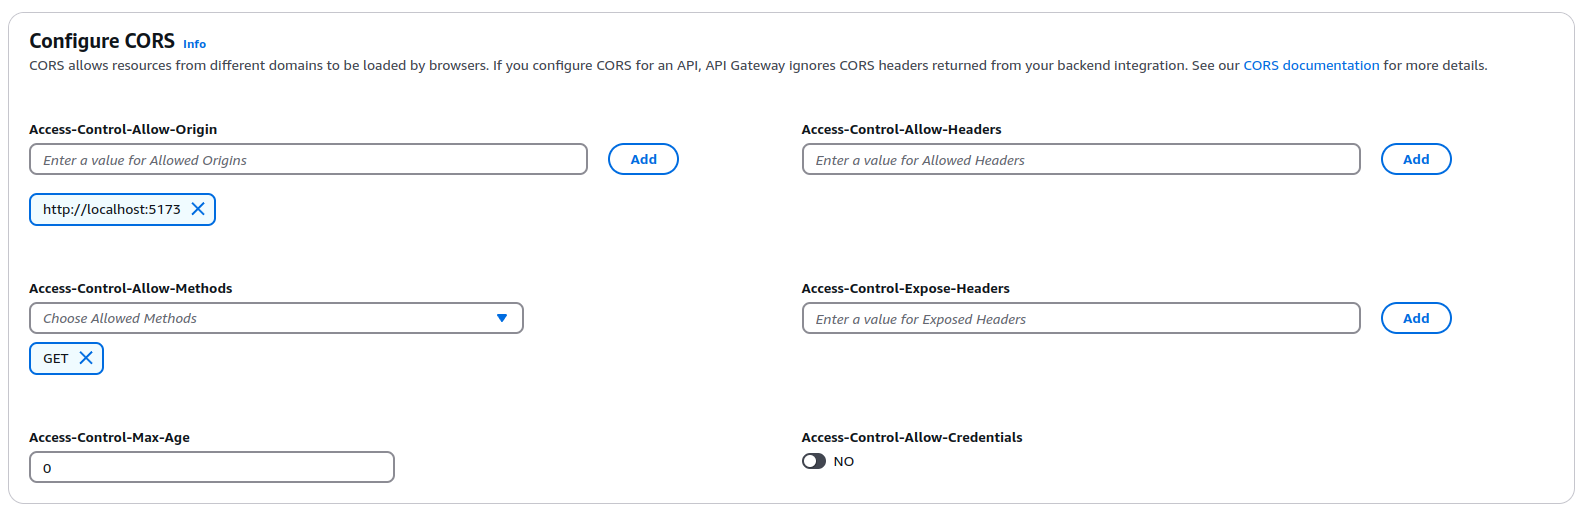
\includegraphics[width=\textwidth]{./images/api_cors_configuration.png}
    \caption{CORS configuration for the HTTP API}
\end{figure}

The Cross-Origin Resource Sharing (CORS) policy accepts only \verb|GET| requests which originate from \url{http://localhost:5173} (the URL of the locally hosted frontend application) to prevent malicious websites from making unauthorised requests on behalf of users to the API.
While the API handles no sensitive data, it is nonetheless best practice to enforce a CORS policy and a ``security-by-default'' approach so that the application does not need to be secured retroactively as its functionality expands.
If the frontend application were moved to a publicly available domain, the URL for this new domain would need to be added to the CORS policy, or else all requests would be blocked.

\subsection{API Endpoints}
\subsubsection{\texttt{/return\_permanent\_data[?objectType=IrishRailStation,BusStop,LuasStop]}}
The \verb|/return_permanent_data| endpoint accepts a comma-separated list of \verb|objectType| query parameters, and returns a JSON response consisting of all items in the permanent data table which match those parameters.
If no query parameters are supplied, it defaults to returning \textit{all} items in the permanent data table.

\subsubsection{\texttt{/return\_transient\_data[?objectType=IrishRailTrain,Bus]}}
The \verb|/return_transient_data| endpoint accepts a comma-separated list of \verb|objectType| query parameters, and returns a JSON response consisting of all the items in the transient data table which match those parameters \textit{and} were uploaded to the transient data table most recently, i.e., the items which have the newest \verb|timestamp| field in the table.
Since the \verb|timestamp| pertains to the batch of data uploaded to the table in a single run, each item in the response will have the same \verb|timestamp| as all the others.
If no \verb|objectType| parameter is supplied, it defaults to returning all items from the newest upload batch. 

\subsubsection{\texttt{/return\_historical\_data[?objectType=IrishRailTrain,Bus]}}
The \verb|/return_historical_data| endpoint functions in the same manner as the \verb|/return_transient_data| endpoint, with the exception that it returns matching items for \textit{all} \verb|timestamp| values in the table, i.e., it returns all items of the given \verb|objectTypes| in the transient data table. 

\subsubsection{\texttt{/return\_luas\_data?luasStopCode=<luas\_stop\_code>}}
The \verb|/return_luas_data| returns incoming / outgoing tram data for a given Luas stop, and is just a proxy for the Luas real-time API.
Since the Luas API returns data only for a queried station and does not give information about individual vehicles, the Luas data for a given station is only fetched on the frontend when a user requests it, as there is no information to plot on the map beyond a station's location.
However, this request cannot be made from the client to the Luas API, as the Luas API's CORS policy blocks requests from unauthorised domains for security purposes;
this API endpoint acts as a proxy, accepting API requests from the \verb|localhost| domain and forwarding them to the Luas API, and subsequently forwarding the Luas API's response back to the client.
\\\\
This endpoint requires a single \verb|luasStopCode| query parameter for each query to identify the Luas stop for which incoming / outgoing tram data is being requested.

\subsubsection{\texttt{/return\_station\_data?stationCode=<station\_code>}}
The \verb|return_station_data| returns information about the trains due into a given station in the next 90 minutes.
This data is only shown to a user if requested for a specific station, so it is not stored in a DynamoDB table.
Like the \verb|/return_luas_data| endpoint, it too is just a proxy for an (Irish Rail) API, the CORS policy of which blocks requests from any unauthorised domain for security purposes.
It requires a single \verb|stationCode| query parameter for each query to identify the train station for which the incoming train data is being requested.

% \subsubsection{\texttt{/return\_punctuality\_by\_objectID[?objectID=<object\_id1>,<object\_id2>]}}
% The \verb|/return_punctuality_by_objectID| endpoint returns the contents of the \verb|punctuality_by_objectID| DynamoDB table. 
% It accepts a comma-separated list of \verb|objectID|s as query parameters, and defaults to returning the average punctuality for \textit{all} items in the table if no \verb|objectID| is specified.

\subsubsection{\texttt{/return\_punctuality\_by\_timestamp[?timestamp=<timestamp>]}}
The \verb|/return_punctuality_by_timestamp| returns the contents of the \verb|punctuality_by_timestamp| DynamoDB table.
It accepts a comma-separated list of \verb|timestamp|s, and defaults to returning the average punctuality for \textit{all} \verb|timestamp|s in the table if no \verb|timestamp| is specified. 

\subsubsection{\texttt{/return\_all\_coordinates}}
The \verb|/return_all_coordinates| endpoint returns a JSON array of all current location co-ordinates in the transient data table for use in statistical analysis.

\section{Serverless Functions}
All the backend code \& logic is implemented in a number of \textbf{serverless functions}\supercite{hassan2021survey}, triggered as needed.
Serverless functions are small, single-purpose units of code that run in the cloud and reduce the need to manage servers \& runtime environments.
In contrast to a server program which is always running, serverless functions are event-driven, meaning that they are triggered by events such as API calls or invocations from other serverless functions and do not run unless triggered.
Each serverless function is \textit{stateless}, which means that each function invocation is independent and that no state data is stored between calls;
they are also \textit{ephemeral}, starting only when triggered and stopping when finished, running only for a short period of time.
This means that they automatically scale up or down depending on usage, and because they only run when they need to, they are much cheaper in terms of compute time than a traditional server application.
\\\\
AWS Lambda\supercite{awslambda} is a serverless compute service provided by Amazon Web Services that allows for the creation of serverless functions without provisioning or managing servers.
A Python AWS Lambda function typically consists of a single source code file with specified entrypoint function, the name of which can vary, but is typically called \verb|lambda_handler()|.
They can be created and managed via the GUI AWS Management Console\supercite{aws_management_console} or via the AWS CLI tool\supercite{aws_cli}.
Each Lambda function can be configured to have a set memory allocation, a timeout duration (how long the function can run for before being killed), and environment variables.
\\\\
Often, when a serverless application replaces a legacy mainframe application, the time \& memory needed to perform routine tasks is drastically reduced because it becomes more efficient to process events individually as they come rather than batching events together to be processed all at once;
the high computational cost of starting up a mainframe system means that it's most efficient to keep it running and to batch process events.
For this reason, serverless functions often require very little memory and compute time.
This application, however, is somewhat unusual as it requires the processing of quite a large amount of data at once:
status updates for public transport don't come from the source APIs individually for each vehicle on an event-by-event basis, but in batches of data that are updated regularly.
Therefore, the serverless functions for this application will require more memory and more compute time to complete.
In this context, memory and compute time have an inversely proportional relationship:
more memory means more items can be processed quickly, thus reducing computational time, and less memory means that fewer items can be processed quickly, thus increasing the computational time.
\\\\
One common approach to tuning the configuration of AWS Lambda functions is to use \textbf{AWS Lambda Power Tuning}\supercite{awsPowerTuning}, an open-source tool that is designed to help optimise the memory \& power configurations for AWS Lambda functions.
It works by invoking the function to be tuned multiple times across various memory allocations, recording metrics such as execution duration and cost for each configuration, and visualises the trade-off between cost and performance for each tested memory configuration, allowing the user to decide the most suitable memory allocation based on minimising cost, maximising speed, or balancing the two.
While this is a very powerful \& useful tool for Lambda function optimisation, it was not used in this project in order to (somewhat ironically) manage costs and remain with the AWS Free Tier:
running the tuner involves several invocations of the target Lambda function at various memory levels, and a typical tuning run involves dozens of Lambda invocations.
With the amount of data being written to the database per Lambda run (thousands of items), this would quickly exceed the free tier and begin incurring costs.
While these costs would not be prohibitively high, doing so would change the nature of the project from researching \& implementing the optimal approach for this application to paying for a faster \& more performant application.
The tuner \textit{could} be run with database writes disabled, but this would not generate meaningful results for the functions as writing to the DynamoDB database is the critical choke point for functions in this application.
\\\\
Instead, each function was manually tuned to consume the least amount of resources (reasonably) possible by gradually incrementing the memory allocation until the function could run to completion in what was deemed to be a reasonable amount of time (somewhat subjectively) for this application;
for this reason, the functions could almost certainly achieve superior execution times if they were allocated more resources, but this would bring the application closer and closer to exceeding the free tier limit of 400,000 GB-seconds (allocated memory in GB $\times$ execution time in seconds).

\subsubsection{\mintinline{python}{fetch_permanent_data}}
The \verb|fetch_permanent_data| Lambda function is used to populate the permanent data table.
As the data in question changes rarely if ever, this function really need only ever be triggered manually, such as when a new train station is opened or a new bus route created.
However, for the sake of completeness and to avoid the data being out of date, a schedule was created with \textbf{Amazon EventBridge} to run the function every 28 days to ensure that no changes to the data are missed.
Like all other schedules created for this application, the schedule is actually disabled at present to avoid incurring unnecessary AWS bills, but can be enabled at any time with the click of a button.

\begin{figure}[H]
    \centering
    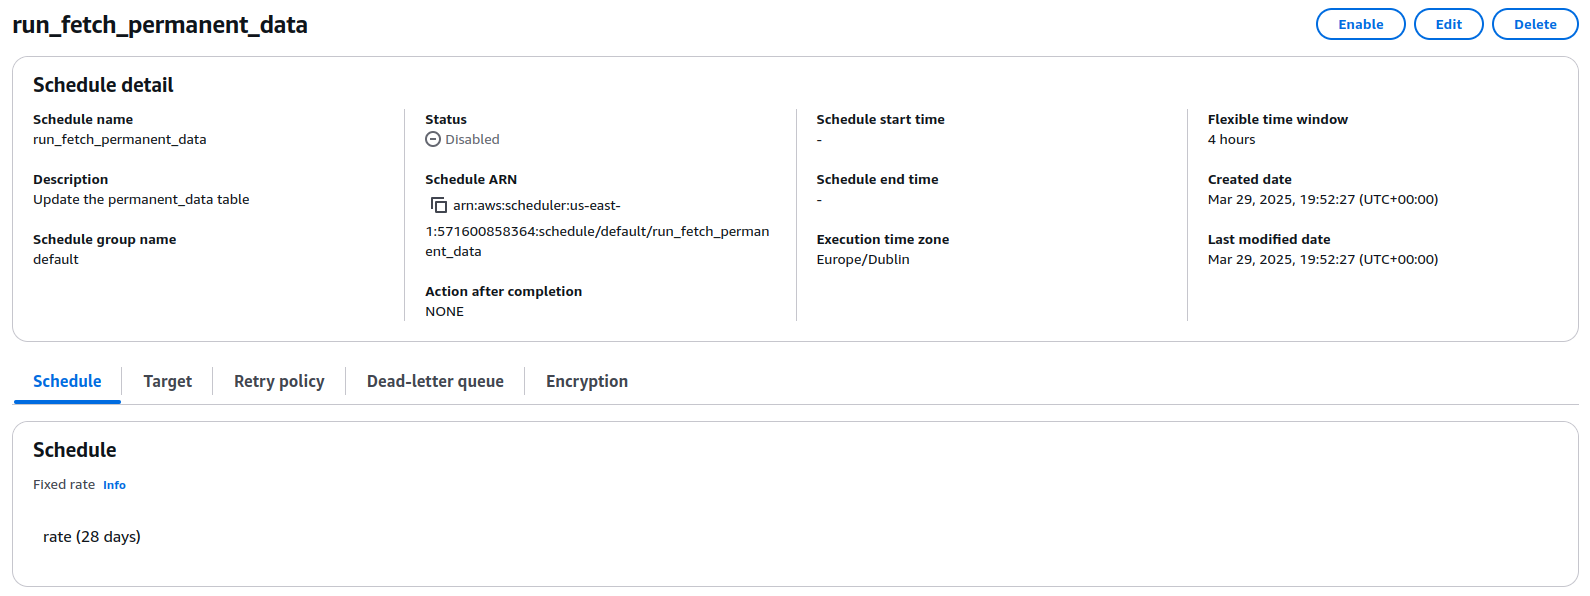
\includegraphics[width=\textwidth]{./images/fetch_permanent_data_schedule.png}
    \caption{Screenshot of the Amazon EventBridge schedule to run the \mintinline{python}{fetch_permanent_data} Lambda function}
\end{figure}

The \verb|fetch_permanent_data| function retrieves Irish Rail Station data directly from the Irish Rail API, but Luas stop data and bus data are not made available through an API;
instead, the Luas stop data is made available online in a tab-separated \verb|TXT| file, and the bus stop \& bus route data are available online in comma-separated \verb|TXT| files distributed as a single ZIP file.
This makes little difference to the data processing however, as downloading a file from a server and parsing its contents is little different in practice from downloading an API response from a server and parsing its contents.
The function runs asynchronously with a thread per type of data being fetched (train station data, Luas stop data, and bus stop \& route data), and once each thread has completed, batch uploads the data to the permanent data table, overwriting its existing contents.

\subsubsection{\mintinline{python}{fetch_transient_data}}
The \verb|fetch_transient_data| function operates much like the \verb|fetch_permanent_data| function, but instead updates the contents of the transient data table.
It runs asynchronously, with a thread per API being accessed to speed up execution;
repeated requests to an API within a thread are made synchronously to avoid overloading the API.
For example, retrieving the type (e.g., Mainline, Suburban, Commuter) of the trains returned by the Irish Rail API requires three API calls:
the Irish Rail API allows the user to query for all trains or for trains of a specific type but it does not return the type of the train in the API response.
Therefore, if a query is submitted for all trains, there is no way of knowing which train is of which type.
Instead, the function queries each type of train individually, and adds the type into the parsed response data.
\\\\
Additionally, the \verb|return_punctuality_by_objectID| function is called when processing the train data so that each train's average punctuality can be added to its data for upload.
Somewhat unintuitively, it transpired that the most efficient way to request this data was to request all data from the punctuality by \verb|objectID| data table rather than individually request each necessary \verb|objectID|;
this means that much of the data returned is redundant, as many of the trains whose punctualities are returned are not running at the time and so will not be uploaded, but it means that the function is only run once, and so only one function invocation, start-up, database connection, and database query have to be created.
It's likely that if bus punctuality data were to become available in the future, this approach would no longer be the most efficient way of doing things, and instead a \verb|return_punctuality_by_objectType| function would be the optimal solution.
\\\\
The bus data API doesn't return any information about the bus route beyond a bus route identifier, so the permanent data table is queried on each run to create a dictionary (essentially a Python hash table\supercite{pythondict}) linking bus route identifiers to information about said bus route (such as the name of the route).
As the bus data is being parsed, the relevant bus route data for each vehicle is inserted.
Once all the threads have finished executing, the data is uploaded in a batch to the transient data table, with each item timestamped to indicate which function run it was retrieved on.
\\\\
This function is run as part of an \textbf{AWS Step Function} with a corresponding Amazon EventBridge schedule (albeit disabled at present).
A step function is an AWS service which facilitates the creation of state machines consisting of various AWS microservices to act as a single workflow.
The state machine allows multiple states and transitions to be defined, with each state representing a step in the workflow and the transitions representing how the workflow moves from one state to another and what data is transferred.
Step functions have built-in error handling and retry functionality, making them extremely fault-tolerant for critical workflows.

\begin{figure}[H]
    \centering
    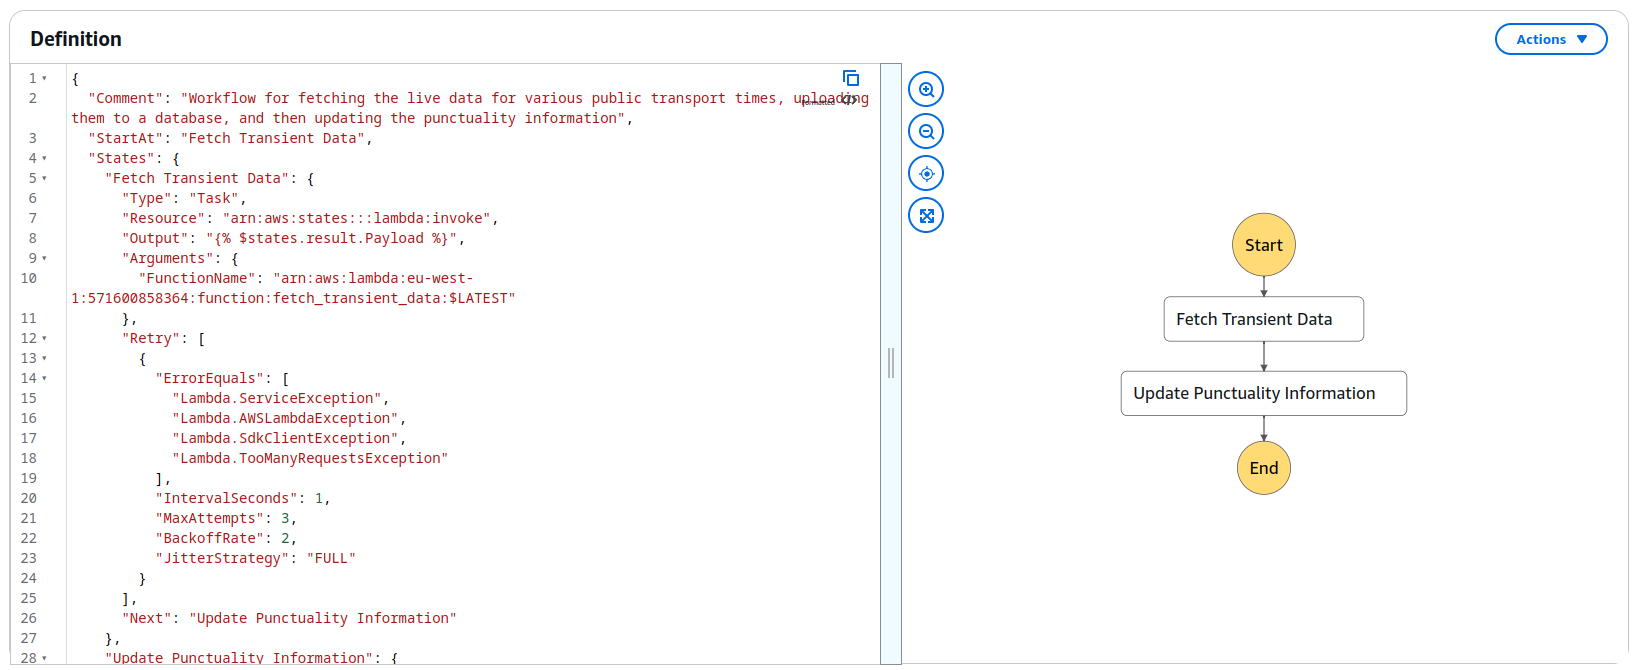
\includegraphics[width=\textwidth]{./images/get_live_data_definiton.png}
    \caption{Screenshot of the \texttt{get\_live\_data} step function definition}
\end{figure}

The step function runs the \verb|fetch_transient_data| function and then runs the \verb|update_average_punctuality| function, if and only if the \verb|fetch_transient_data| function has completed successfully.
This allows the average punctuality data to be kept up to date and in sync with the transient data, and ensures that they do not become decoupled and therefore incorrect.
This step function is triggered by a (currently disabled) Amazon EventBridge schedule which runs the function once a minute, which is the maximum frequency possible to specify within a cron schedule, and suitable for this application as the APIs from which the data is sourced don't update much more frequently than that.
Furthermore, the data from which bus data is sourced will time out if requests are made too frequently, so this value was determined to be appropriate after testing to avoid overwhelming the API or getting timed-out. 
It is possible to run EventBridge schedules even more frequently using the \textit{rate-based schedule} schedule type instead of the \textit{cron-based schedule} schedule type but a more frequent schedule would be inappropriate for this application.

\subsubsection{\mintinline{python}{update_average_punctuality}}
The \verb|update_average_punctuality| function runs after \verb|fetch_transient_data| in a step function and populates the average punctuality by \verb|objectID| and average punctuality by \verb|timestamp| tables to reflect the new data collected by \verb|fetch_transient_data|.
For each item in the new data, it updates the average punctuality in the average punctuality by \verb|objectID| table according to the aforementioned formula:
\[
  \bar{x}_{\text{new}} = \frac{\left( \bar{x}_\text{old} + c \right) + x}{c + 1}
\]

As the function iterates over each item, it adds up the total punctuality and then divides this by the total number of items processed before adding it to the average punctuality by \verb|timestamp| table, where the \verb|timestamp| in question is the \verb|timestamp| that the items were uploaded with (the \verb|timestamp| of the \verb|fetch_transient_data| run which created them).
\\\\
There are a number of concerns that one might reasonably have about using the mean punctuality for the average displayed to users:
\begin{itemize}
  \item   Means are sensitive to outliers, meaning that if, for example, a train is very late just once but very punctual the rest of the time, its average punctuality could be misleading.
  \item   The punctuality variable is an integer that can be positive or negative, which could have the result that the positive \& negative values could cancel each other out for a train that is usually either very late or very early, giving the misleading impression of an average punctuality close to zero.
  \item   Considering the entire history of a train for its average punctuality may not be reflective of recent trends:
          a train may historically have been consistently late, but become more punctual as of late and therefore the average punctuality may not be reflective of its recent average punctuality. 
\end{itemize}

These questions were carefully considered when deciding how to calculate the average punctuality, but it was decided that the mean would nonetheless be the most appropriate for various reasons:
\begin{itemize}
  \item   The mean lends itself to efficient calculation with the $O(1)$ formula described above.
          No other average can be calculated in so efficient a manner:
          the median requires the full list of punctualities to be considered to determine the new median, and the mode requires at the very least a frequency table of all the punctualities over time to determine the new mode, which requires both additional computation and another DynamoDB table.

  \item   Similarly, considering only recent data would destroy the possibility for efficient calculation:
          the mean could not be updated incrementally, and instead a subset of the historic punctualities would have to be stored and queried for each update.

  \item   The outlier sensitivity is addressed by the sheer number of items that are considered for the mean:
          since this will be updated every minute of every day, an outlier will quickly be drowned out with time.

  \item   Finally, the average is being calculated so that it can be shown to the user and so that they can make decisions based off it.
          The average person from a non-technical or non-mathematical background tends to assume that any average value is a mean value, and so it would only serve to confuse users if they were given some value that did not mean what they imagined it to mean.
          While calculating additional different measures of averages would be possible, displaying them to the user would likely be at best not useful and at worst confusing, while also greatly increasing the computation and storage costs.
          This aligns with the second of Nielsen's famous \textit{10 Usability Heuristics for User Interface Design}, which were consulted throughout the design process: ``\textbf{Match between the System and the Real World:} The design should speak the users' language. Use words, phrases, and concepts familiar to the user, rather than internal jargon''\supercite{nielsenheuristics}.
\end{itemize}

For these reasons, it was decided that the mean was the most suitable average to use.

\subsubsection{\mintinline{python}{return_permanent_data}}
The \verb|return_permanent_data| function is the Lambda function which is called when a request is made from the client to the \verb|/return_permanent_data| API endpoint.
It checks for a comma-separated list of \verb|objectType| parameters in the query parameters passed from the API event to the Lambda function, and scans the permanent data table for every item matching those \verb|objectType|s.
If none are provided, it returns every item in the table, regardless of type.
It returns this data as a JSON string.
\\\\
When this function was first being developed, the permanent data table was partitioned by \verb|objectID| alone with no sort key, meaning that querying was very inefficient.
When the table was re-structured to have a composite primary key consisting of the \verb|objectType| as the partition key and the \verb|objectID| as the sort key, the \verb|return_permanent_data| function was made 10$\times$ faster:
the average execution time was reduced from $\sim$10 seconds to $\sim$1 second, demonstrating the critical importance of choosing the right primary key for the table.

\subsubsection{\mintinline{python}{return_transient_data}}
The \verb|return_transient_data| function is the Lambda function which is called when a request is made from the client to the \verb|/return_transient_data| API endpoint.
Like \verb|return_permanent_data|, it checks for a comma-separated list of \verb|objectType| parameters in the query parameters passed from the API event to the Lambda function, and scans the permanent data table for every item matching those \verb|objectType|s.
If none are provided, it returns every item in the table, regardless of type.
\\\\
Similar to \verb|return_permanent_data|, when this function was originally being developed, there was no GSI on the transient data table to facilitate efficient queries by \verb|objectType| and \verb|timestamp|;
the addition of the GSI and updating the code to exploit the GSI resulted in an average improvement in run time of $\sim$8$\times$, thus demonstrating the utility which GSIs can provide.

\subsubsection{\mintinline{python}{return_punctuality_by_objectID}}
The \verb|return_punctuality_by_objectID| function is invoked by the \verb|fetch_transient_data| function to return the contents of the punctuality by \verb|objectID| table. 
It accepts a list of \verb|objectID|s and defaults to returning all items in the table if no parameters are provided.

\subsubsection{\mintinline{python}{return_punctuality_by_timestamp}}
The \verb|return_punctuality_by_timestamp| function is similar to \verb|return_punctuality_by_objectID| but runs when invoked by an API request to the \verb|/return_punctuality_by_timestamp| endpoint and simply returns a list of JSON objects consisting of a \verb|timestamp| and an \verb|average_punctuality|.
It is used primarily to graph the average punctuality of services over time.

\subsubsection{\mintinline{python}{return_all_coordinates}}
The \verb|return_all_coordinates| function is used to populate the co-ordinates heatmap in the frontend application which shows the geographical density of services at the present moment.
It accepts no parameters, and simply scans the transient data table for the newest items and returns their co-ordinates.

\subsubsection{\mintinline{python}{return_historical_data}}
The \verb|return_historical_data| function operates much like the \verb|return_transient_data| function, accepting a list of \verb|objectType|s or defaulting to all \verb|objectType|s if none are specified, with the only difference being that this function does not consider the \verb|timestamp|s of the data and just returns all data in the transient data table.
This function, along with its corresponding API endpoint exist primarily as a debugging \& testing interface, although they also give a convenient access point for historical data analysis should that be necessary.

\subsubsection{\mintinline{python}{return_luas_data}}
The \verb|return_luas_data| function is a simple proxy for the Luas API which accepts requests from the client and forwards them to the Luas API to circumvent the Luas API's restrictive CORS policy which blocks requests from unauthorised domains.
It simply accepts a \verb|luasStopCode| parameter, and makes a request to the Luas API with said parameter, parses the response from XML into JSON, and returns it.

\subsubsection{\mintinline{python}{return_station_data}}
Like \verb|return_luas_data|, the \verb|return_station_data| is a proxy for the Irish Rail API so that requests can be made as needed from the client's browser to get data about incoming trains due into a specific section without running afoul of Irish Rail's CORS policy.
It also accepts a single parameter (\verb|stationCode|) and makes a request to the relevant endpoint of the Irish Rail API, and returns the response (parsed from XML to JSON).

\section{CI/CD Pipeline}
\subsection{Unit Tests}
As the code for each Lambda function was written, so too were corresponding PyUnit\supercite{pyunit} (based on the Java unit testing framework JUnit\supercite{junit}) unit tests for that function to ensure that the function was working as expected, that edge cases were covered, and to indicate if functionality was broken when updates were made.
Indeed, this often proved invaluable, as the unit tests revealed on multiple occasions edge cases that were not handled properly, such as the handling of the API responses when only a single item was returned.
Without the utilisation of unit testing, it's likely that these issues would have gone unnoticed in the codebase until they caused an error in deployment, which could have lead to Lambda function crashes, inconsistent database data, and wasted developer time spent on debugging the application.
\\\\
These PyUnit tests are run using \mintinline{python}{pytest}\supercite{pytest} which automatically discovers Python test files in a given directory and can generate code coverage reports.
While PyUnit tests can be run with \mintinline{shell}{python -m unittest}, \mintinline{python}{pytest} makes it easier to run the tests and can generate coverage reports automatically.
\mintinline{python}{pytest} also allows for unit tests to be specified in its own non-standard format alongside to the standard PyUnit format, but this was not used in an effort to keep the tests as standard and as homogeneous as possible.
The coverage percentage is calculated as:
\begin{align*}
    \text{Coverage (\%)} = \frac{\text{Number of lines executed}}{\text{Total number of executable lines}} \times 100
\end{align*}
A line coverage of 70\% was selected to be aimed for when writing tests for this application;
this is a high degree of test coverage, but allows the tests to focus on testing the core logic of the application rather than boilerplate code and allows for interactions with third-party services that cannot be fully covered by testing and instead have to be mocked\supercite{pyunitmock}.
The actual total coverage achieved is 85\%, which exceeds this minimum value and ensures that the application is well-covered with test cases.

\begin{figure}[H]
    \centering
    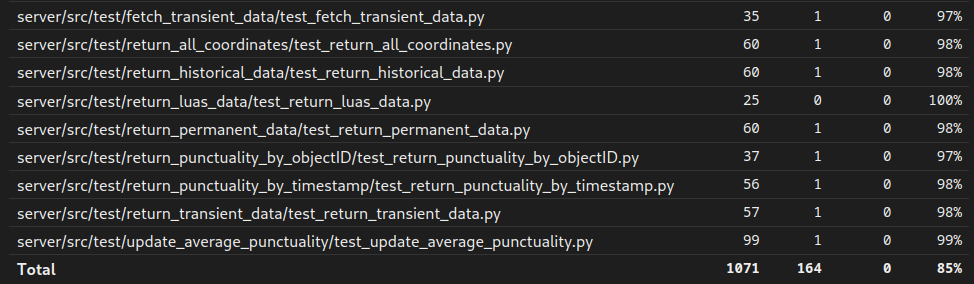
\includegraphics[width=\textwidth]{./images/testcoverage.png}
    \caption{Screenshot of (some of) the results from the HTML coverage report generated}
\end{figure}

\subsection{CI/CD}
To run the unit tests automatically, a GitHub Workflow\supercite{workflow} was created.
This workflow is triggered when a pull request to merge code into the \verb|main| Git branch is opened, or when code is pushed to the \verb|main| branch.
Since the Git repository used for this project is a monorepo containing all code files for the project, not just the backend Python files, many of the commits to this repository will not require re-running the unit tests, as the Python code will not have changed;
therefore, the workflow only runs if the changes have been made to a \verb|*.py| file.

\begin{code}
\begin{minted}[linenos, breaklines, frame=single]{yaml}
name: Continuous Integration / Continuous Deployment

on:
  pull_request:
    branches:
      - main
    paths:
      - "**.py"
  push:
    branches:
      - main
    paths:
      - "**.py"
\end{minted}
\caption{Snippet of the \texttt{ci.yml} workflow file}
\end{code}

The workflow consists of two ``jobs'':
\begin{itemize}
    \item   The \verb|test| job installs the necessary dependencies and runs the unit tests, generating coverage reports in both XML and HTML and uploading these as artifacts\supercite{artifacts} (a way to share data from a GitHub workflow run).
    \item   The \verb|deploy| job runs only on pushes to \verb|main| (including direct pushes and merges of pull requests), and only runs if the \verb|test| job completed successfully: if any of the tests fail, the code will not be deployed and an email will be sent to the administrators of the GitHub repository.
            It installs AWS CLI\supercite{aws_cli} and sets the AWS credentials using GitHub Secrets\supercite{githubsecrets} which allow for sensitive information such as environment variables to be stored privately for a repository, even if that repository is public, and avoids having to hard-code these values.
            It then iterates over each Lambda function in the repository, installs the necessary Python libraries to a temporary directory, and bundles these along with the function source code into a ZIP file for deployment via the AWS CLI. 
\end{itemize}

\chapter{Frontend Design \& Implementation}
The frontend design is built following the Single-Page-Application (SPA)\supercite{spa} design pattern using the React Router\supercite{reactrouter} library, meaning that the web application loads a single HTML page and dynamically updates content as the user interacts with the application, without reloading the webpage. 
Since there is just one initial page load, the content is dynamically updated via the DOM using JavaScript rather than by requesting new pages from the server;
navigation between pseudo-pages is managed entirely using client-side routing for a smoother \& faster user experience since no full-page reloads are necessary.
\\\\
The web application is split into three ``pages'':
\begin{itemize}
  \item   The home (or map) page, which is the main page that displays live location data \& service information to the user.
          This page is where the user will spend the majority of their time, and where the majority of the functionality is delivered.
  \item   The statistics page, which is used to deliver statistical insights about the data to the user.
          This page is for providing deeper insights into the stored data on a collective basis, rather than on a per-service basis.

      \item   The help page, which gives some basic usage information on how to complete basic tasks within the application, in keeping with Nielsen's usability heuristic of ``Help and Documentation''\supercite{nielsenheuristics}.
\end{itemize}

The web application follows the Container/Presentational Pattern\supercite{containerpresentational}, which enforces separation of concerns by separating the presentational logic from the application logic.
This is done by separating the functionality into two classes of components:
\begin{itemize}
  \item   \textbf{Container Components:} those which fetch the data, process it, and pass it to the presentational components which are contained by their container components, i.e., the presentational components are children of the container components.
  \item   \textbf{Presentational Components:} those which display the data it receives from the container components to the user as it is received.
          This makes the components highly re-usable, as there isn't specific data handling logic within them.
\end{itemize}

React components are reusable, self-contained pieces of the UI which act as building blocks for the application\supercite{reactcomponents};
they can receive properties from their parent components, manage their own internal state, render other components within themselves, and respond to events.
\\\\
The Container/Presentational pattern can be contrasted with other design patterns for UI design such as the Model-View-Controller (MVC) pattern\supercite{reenskaug2003mvc}:
in many ways, the containers of the Container/Presentational pattern as a collective can be thought of as analogous to the controller of the MVC pattern, and the presentational components as analogous to the view.
The key difference between the two patterns is that the Container/Presentational pattern defines only the architecture of the frontend layer, and does not dictate how the backend ought to be laid out;
the MVC pattern defines the architecture of the entire application and so the backend (the model) is necessarily \textit{tightly coupled}\supercite{mcnatt2001coupling} with the frontend layer (the view) by means of the controller.
Therefore, updating the backend code will most likely necessitate updating the frontend code (and vice-versa).
For this reason, MVC is most commonly used for applications in which the backend \& the frontend are controlled by the same codebase, and especially for application in which the frontend rendering is done server-side.
The Container/Presentational pattern, however, is \textit{loosely coupled}\supercite{mcnatt2001coupling} with the backend and therefore the frontend \& the backend can be updated almost independently of one another as long as the means \& format of data transmission remain unchanged, thus making development both faster \& easier, and mitigating the risk of introducing breaking changes.
The Container/Presentational pattern lends itself particularly well to React development, as React code is rendered client-side and makes extensive use of components: the Container/Presentational pattern just ensures that this use of components is done in a way that is logical \& maintainable.

\section{Main Page}
\begin{figure}[H]
    \centering
    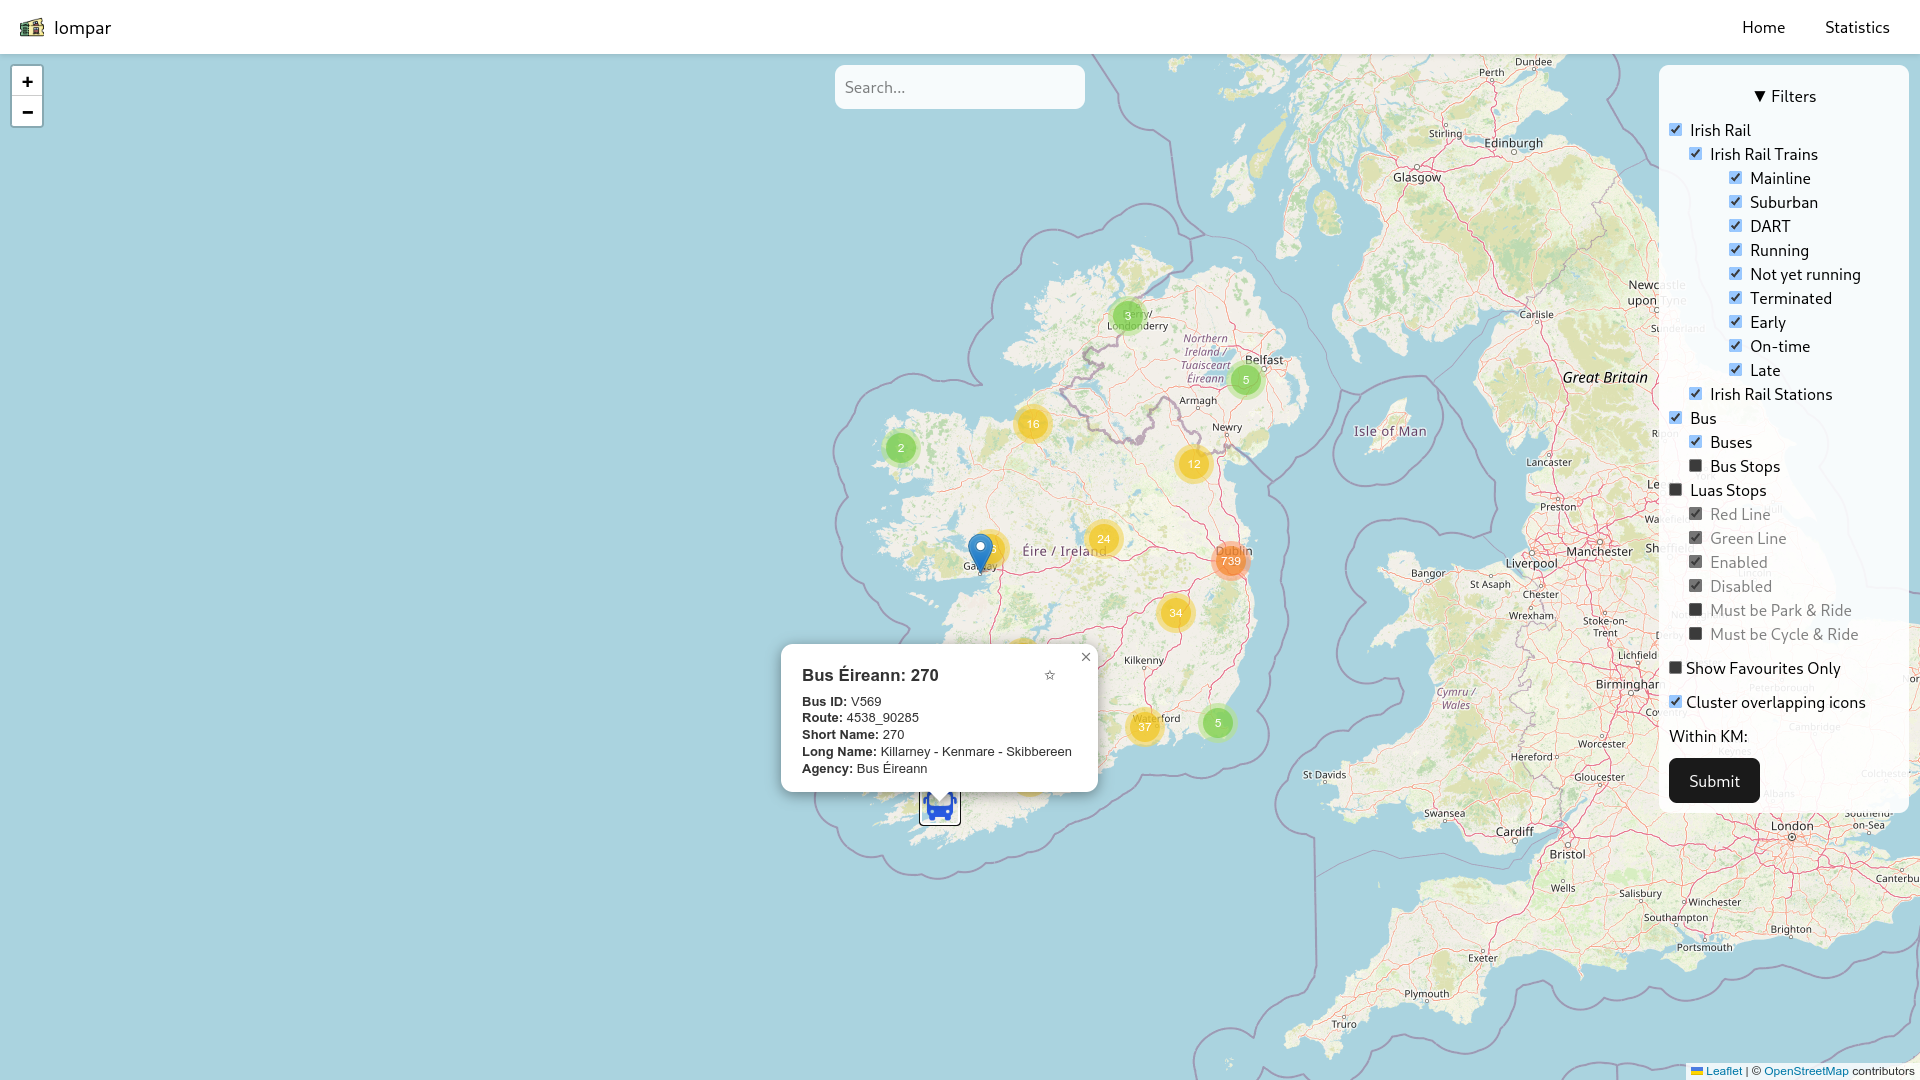
\includegraphics[width=\textwidth]{./images/mainpage.png}
    \caption{Screenshot of the front page of the web application}
\end{figure}

The main page of the application contains a map upon which the live location of each public transport object is marked, a navigation bar, a search bar to filter the vehicles shown on the map, and a filters side-panel which allows the user to select what kind of objects the user wants displayed on the map.
The location markers for each item are clickable, and when clicked, display a pop-up with relevant information about the selected item.
In line with Container/Presentational pattern, the main \verb|App.jsx| file contains the data retrieval \& processing logic, and passes the processed data to presentational components for display. 

\subsubsection{Data Retrieval \& Processing}
The data is retrieved and processed in a function named \mintinline{javascript}{fetchData()}.
When the ``Submit'' button is clicked in the filters side-panel, the function is triggered and sends asynchronous API requests to the \verb|/return_permanent_data| and \verb|/return_transient_data| API endpoints as necessary.
The \verb|App.jsx| file contains a JavaScript object which identifies what checkboxes in the side-panel pertain to \verb|objectType|s in the backend, and which API endpoint they can be sourced from.
When the function is fetching data, it constructs a comma-separated list of selected \verb|objectType|s to send to each API endpoint, thereby making only one request to each API endpoint to avoid unnecessary repeated queries.
\\\\
Originally, the returned data was processed using JavaScript functional array methods\supercite{arraymethods} (very superficially similar to the Java \mintinline{java}{Stream}\supercite{javastream} interface), which allow for the creation of chained operations on arrays, not dissimilar to chained shell operations using the pipe (\mintinline{shell}{|}) operator on UNIX-like systems\supercite{redhatpipe}.
Methods like \mintinline{javascript}{.map()}, \mintinline{javascript}{.reduce()}, etc. are some of the methods covered in JavaScript functional array methods which allow data processing pipelines to be specified in a clean, elegant, \& readable manner.
However, the price of this elegance is slower and less efficient execution:
these array methods add extra layers of abstraction, invoke a new function per element, create intermediate arrays for each result, and (unlike their Java counterparts) do not support short-circuiting and therefore cannot break early (with the exception of the \mintinline{javascript}{.some()} \& \mintinline{js}{.many()} methods)\supercite{shortcircuit}.
The modern JavaScript engine also is less efficient at optimising these array methods than simple \mintinline{javascript}{for}-loops\supercite{jsmethodopti}.
Indeed, re-writing the function to use a simple \mintinline{js}{for} loop resulted in an average loading speed increase of $\sim$2 seconds when all data sources were selected. 
\\\\
While the data is loading, a loading overlay with a ``spinner'' icon is displayed on-screen which prevents the user from interacting with the UI, keeps the user informed of what's going on (in keeping with the first of Nielsen's 10 usability heuristics\supercite{nielsenheuristics}), prevents the user from changing any settings as the data is loaded that may cause inconsistent behaviour, and gives the perception of a smoother loading experience.
Studies have shown that displaying a loading screen to the user instead of just waiting for the UI to update gives the impression of a faster loading speed, so much so that even longer load times with a loading screen feel faster than shorter load times without one\supercite{mdnperceivedperformance, persson2019perceived, Vladic2020LoadingAnimations}.
\\\\
Once the JSON response is received, each item in the response is iterated over, as described above, and the marker for each item is constructed.
The map plotting is done with Leaflet\supercite{leaflet}, and each marker on the map consists of an array of co-ordinates, some HTML pop-up content when the marker is clicked, an icon depending on the transport type, a Boolean display variable which dictates whether or not the marker is displayed, and some markup-free \mintinline{js}{markerText} which is not part of the Leaflet API\supercite{leaflet} but added to each icon to give it some text to which the search text can be compared.
This \mintinline{js}{markerText} is never displayed to the user, and is used solely for search \& filtering purposes;
it is created as an additional variable instead of just using the pop-up content for searching as the pop-up content contains HTML mark-up which would have to be removed at search time to make searching possible, leading to a large number of unnecessary \& costly string-processing operations.
Each item has a colour-coded icon depending on the type of data it represents:

\begin{table}[H]
  \centering
  \begin{tabular}{|>{\centering\arraybackslash}m{1.8cm}|m{10cm}|}
    \hline
    \vspace{2mm}
\includegraphics[width=1cm]{../frontend/src/assets/icons/train_ontime.png}\supercite{trainicon} & On-time \& early, running Irish Rail trains\\
    \hline
    \vspace{2mm}
\includegraphics[width=1cm]{../frontend/src/assets/icons/train_late.png}\supercite{trainicon}  & Late, running Irish Rail trains\\
    \hline
    \vspace{2mm}
\includegraphics[width=1cm]{../frontend/src/assets/icons/train.png}\supercite{trainicon}  & Not-yet running \& terminated Irish Rail trains\\
    \hline

    \vspace{2mm}
\includegraphics[width=1cm]{../frontend/src/assets/icons/DARTOnTime.png}\supercite{darticon} & On-time \& early, running DARTs\\
    \hline
    \vspace{2mm}
\includegraphics[width=1cm]{../frontend/src/assets/icons/DARTLate.png}\supercite{darticon}  & Late, running DARTs\\
    \hline
    \vspace{2mm}
\includegraphics[width=1cm]{../frontend/src/assets/icons/DARTnotRunning.png}\supercite{darticon}  & Not-yet running \& terminated DARTs\\
    \hline


    \vspace{2mm}
\includegraphics[width=1cm]{../frontend/src/assets/icons/train-station.png}\supercite{trainstaitionicon} & Irish Rail stations \\
    \hline

    \vspace{2mm}
\includegraphics[width=1cm]{../frontend/src/assets/icons/bus.png}\supercite{busicon} & Buses \\
    \hline
    \vspace{2mm}
\includegraphics[width=1cm]{../frontend/src/assets/icons/bus-station.png}\supercite{busstopicon} & Bus stops \\
    \hline

    \vspace{2mm}
\includegraphics[width=1cm]{../frontend/src/assets/icons/luasRed.png}\supercite{tramicon} & Red line Luas stops \\
    \hline
    \vspace{2mm}
\includegraphics[width=1cm]{../frontend/src/assets/icons/luasGreen.png}\supercite{tramicon} & Green line Luas stops \\
    \hline
  \end{tabular}
  \caption{Marker icons \& their descriptions}
\end{table}

The value of the Boolean \verb|display| variable for each function is calculated before any pop-up content or \verb|markerText| is generated, so as not to waste computational time generating information that will not be shown to the user. 
Each \verb|objectType| has its own Boolean formula that determines whether or not an item should be shown to the user, depending on what filters they have selected.
Each formula is constructed in such a way that expensive computations are avoided if they are unnecessary, by taking advantage of JavaScript's ability to \textbf{short-circuit} logical expressions, that is, return immediately if the left-hand side of a Boolean \verb|AND| is false\supercite{logicaland} or if the left-hand side of a Boolean \verb|OR| is true\supercite{logicalor}.


\begin{align*}
\text{display}_{\text{train}} =\quad
& (\text{latitude} \neq 0) \land (\text{longitude} \neq 0) \\
& \land \big( (\text{showMainline} \land (\text{trainType} = \text{Mainline})) \\
& \quad\ \ \lor (\text{showSuburban} \land (\text{trainType} = \text{Suburban})) \\
& \quad\ \ \lor (\text{showDart} \land (\text{trainType} = \text{DART})) \big) \\
& \land \big( (\text{showRunning} \land (\text{trainStatus} = \text{Running})) \\
& \quad\ \ \lor (\text{showNotYetRunning} \land (\text{trainStatus} = \text{Not yet running})) \\
& \quad\ \ \lor (\text{showTerminated} \land (\text{trainStatus} = \text{Terminated})) \big) \\
& \land \big( ((\text{trainStatus} = \text{Running}) \land \\
& \quad\ \ \ \ ((\text{showEarly} \land (\text{trainPunctualityStatus} = \text{early})) \\
& \quad\quad\quad\ \ \lor (\text{showOnTime} \land (\text{trainPunctualityStatus} = \text{On time})) \\
& \quad\quad\quad\ \ \lor (\text{showLate} \land (\text{trainPunctualityStatus} = \text{late})))) \\
& \quad\ \ \lor ((\text{trainStatus} = \text{Not yet running}) \land \text{showNotYetRunning}) \\
& \quad\ \ \lor ((\text{trainStatus} = \text{Terminated}) \land \text{showTerminated}) \big) \\
& \land \big( (\text{withinDistance} \land \text{userLocationAvailable}) \Rightarrow \\
& \quad\quad\ \ \text{haversineDistance}(\text{userLocation}, [\text{latitude}, \text{longitude}]) < \text{withinDistance} \big) \\
& \land \left( \text{showFavouritesOnly} \Rightarrow \text{trainCode} \in \text{favourites} \right)
\end{align*}

\begin{align*}
\text{display}_{\text{station}} =\quad
& (\text{latitude} \neq 0) \land (\text{longitude} \neq 0) \\
& \land \big( (\text{withinDistance} \land \text{userLocationAvailable}) \Rightarrow \\
& \quad\quad\ \ \text{haversineDistance}(\text{userLocation}, [\text{latitude}, \text{longitude}]) < \text{withinDistance} \big) \\
& \land \left( \text{showFavouritesOnly} \Rightarrow \text{trainStationCode} \in \text{favourites} \right)
\end{align*}

\begin{align*}
\text{display}_{\text{bus}} =\quad
& (\text{latitude} \neq 0) \land (\text{longitude} \neq 0) \\
& \land \big( (\text{withinDistance} \land \text{userLocationAvailable}) \Rightarrow \\
& \quad\quad\ \ \text{haversineDistance}(\text{userLocation}, [\text{latitude}, \text{longitude}]) < \text{withinDistance} \big) \\
& \land \left( \text{showFavouritesOnly} \Rightarrow \text{busRoute} \in \text{favourites} \right)
\end{align*}

\begin{align*}
\text{display}_{\text{bus stop}} =\quad
& (\text{latitude} \neq 0) \land (\text{longitude} \neq 0) \\
& \land \big( (\text{withinDistance} \land \text{userLocationAvailable}) \Rightarrow \\
& \quad\quad\ \ \text{haversineDistance}(\text{userLocation}, [\text{latitude}, \text{longitude}]) < \text{withinDistance} \big) \\
& \land \left( \text{showFavouritesOnly} \Rightarrow \text{busStopID} \in \text{favourites} \right)
\end{align*}

\begin{align*}
\text{display}_{\text{Luas stop}} =\quad
& (\text{latitude} \neq 0) \land (\text{longitude} \neq 0) \\
& \land \big( (\text{showGreenLine} \land (\text{luasLine} = \text{Green Line})) \\
& \quad\ \ \lor (\text{showRedLine} \land (\text{luasLine} = \text{Red Line})) \big) \\
& \land \big( (\text{showEnabled} \land (\text{luasStopIsEnabled} = 1)) \\
& \quad\ \ \lor (\text{showDisabled} \land (\text{luasStopIsEnabled} = 0)) \big) \\
& \land \big( \neg \text{showCycleAndRide} \lor (\text{showCycleAndRide} \land (\text{luasStopIsCycleAndRide} = 1)) \big) \\
& \land \big( \neg \text{showParkAndRide} \lor (\text{showParkAndRide} \land (\text{luasStopIsParkAndRide} = 1)) \big) \\
& \land \big( (\text{withinDistance} \land \text{userLocationAvailable}) \Rightarrow \\
& \quad\quad\ \ \text{haversineDistance}(\text{userLocation}, [\text{latitude}, \text{longitude}]) < \text{withinDistance} \big) \\
& \land \left( \text{showFavouritesOnly} \Rightarrow \text{luasStopID} \in \text{favourites} \right)
\end{align*}

Although the formulae may appear excessively complex at first glance, they're relatively easy to understand when broken down:
each line is essentially a conjunction of a variable that dictates whether or not a filter is applied and a check to see if that condition is fulfilled, e.g., $(\text{showMainline} \land (\text{trainType} = \text{Mainline}))$ checks if the ``Show Mainline'' filter is applied and if the item in question fulfils that criterion.
Each line of logic is either in conjunction or disjunction with the preceding line depending on whether or not that the filter is a \textit{permissive filter} (that is, it increases the number of items shown) or if it is a \textit{restrictive filter} (that is, it decreases the number of items shown).
\\\\
As can be seen in the preceding formulae, if the user location is available and the user has specified that all items must be within a certain distance of their location, each marker is checked to see if it's within range by using \textbf{Haversine distance}, which calculates the shortest distance between two points on the surface of a sphere.
The Haversine distance formula is defined as follows\supercite{chopde2013landmark}:
\begin{align*}
d = 2r \cdot \arcsin \left( \sqrt{ \sin^2 \left( \frac{\Delta \phi}{2} \right) + \cos \left( \phi_1 \right) \cos \left( \phi_2 \right) \sin^2 \left( \frac{\Delta \lambda}{2} \right) } \right)
\end{align*}
where:
\begin{itemize}
  \item   $d$ is the distance between the two points,
  \item   $r$ is the radius of the Earth ($\sim$6,371 kilometres\supercite{turcotte_earths_radius_1992}),
  \item   $\phi_1, \phi_2$ are the latitudes of each point in radians,
  \item   $\lambda_1, \lambda_2$ are the longitudes of each point in radians,
  \item   $\Delta \phi = \phi_2 - \phi_1$, and
  \item   $\Delta \lambda = \lambda_2 - \lambda_1$.
\end{itemize}

This formula was chosen as a good middle ground between accurate distance calculations and efficient computation.
There are other distance formulae, such as Vincenty's formula\supercite{vincenty1975geodesics} which is more accurate (because it considers the Earth to be an oblate spheroid rather than sphere) but slower to compute, or Euclidean distance\supercite{smith2013precalculus} which is fast to compute, but inaccurate for points on the surface of the Earth (because it considers the points to be on flat 2D grid).
Arguably, one could get away with using Euclidean distance, as the distances considered in this application are relatively short (covering only the island of Ireland) and in general, a user will be specifying only short distances to see services in their immediate vicinity.
However, this approach cannot be scaled if the application scope was increased to include a broader geographical area as inaccuracies would rapidly build up, and even over the island of Ireland alone, there is potential for inconsistent behaviour due to measurement inaccuracies.  
Haversine distance is not too computationally expensive, and guarantees a reliable degree of accuracy for the user.

\subsubsection{Marker Pop-Ups}
\begin{figure}[H]
    \centering
    % Row 1
    \begin{subfigure}[c]{0.3\textwidth}
        \centering
        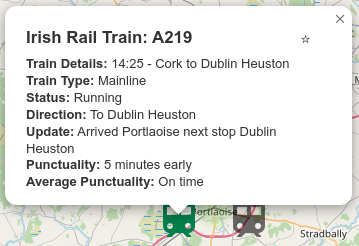
\includegraphics[width=\textwidth]{./images/irishrailtrainpopup.png}
        \caption{\texttt{IrishRailTrain} pop-up}
    \end{subfigure}
    \hfill
    \begin{subfigure}[c]{0.3\textwidth}
        \centering
        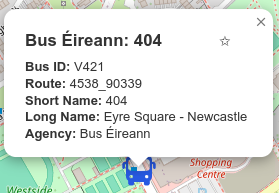
\includegraphics[width=\textwidth]{./images/buspopup.png}
        \caption{\texttt{Bus} pop-up}
    \end{subfigure}
    \hfill
    \begin{subfigure}[c]{0.3\textwidth}
        \centering
        
\includegraphics[width=\textwidth]{./images/busstoppopup.png}
        \caption{\texttt{BusStop} pop-up}
    \end{subfigure}

    \vspace{0.5cm} % space between rows

    % Row 2
    \begin{subfigure}[c]{0.3\textwidth}
        \centering
        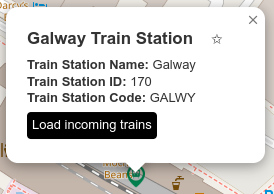
\includegraphics[width=\textwidth]{./images/irishrailstationpopup.png}
        \caption{\texttt{IrishRailStation} pop-up}
    \end{subfigure}
    \hfill
    \begin{subfigure}[c]{0.3\textwidth}
        \centering
        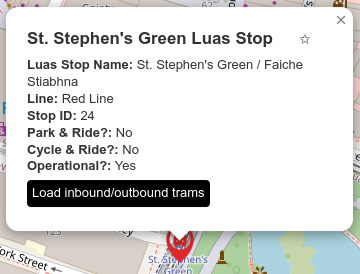
\includegraphics[width=\textwidth]{./images/luasstoppopup.png}
        \caption{\texttt{LuasStop} pop-up}
    \end{subfigure}
    \hfill

    \caption{The 5 pop-up types}
\end{figure}

When the data is being fetched, a pop-up is created for each new marker collected, to be displayed when the marker is clicked. 
For each \verb|objectType|, there is a separate React component for its pop-up to which the item's data is passed so that it can be rendered differently depending on the service type.
The \verb|IrishRailTrain| pop-up, \verb|Bus| pop-up, \& \verb|BusStop| are the most similar and the simplest, as they simply display information passed into their respective components, the only variance being that different \verb|objectType|s have different fields to display.
\\\\
Each pop-up has a ``star'' button which, when clicked, adds the selected item to a list of the user's ``favourite'' services, which is stored as a cookie in the user's browser.
This cookie is loaded when the main page is loaded and updated every time an item is toggled to be ``starred'' or not.
This list of favourites is used to determine whether or not the item is displayed when the user selects ``Show favourites only'', as can be seen in the Boolean display formulae previously outlined.
Favouriting behaves differently depending on the \verb|objectType| of the item being favourited:
notably, buses are favourited not on a per-vehicle basis using the item's \verb|objectID|, but on a per-route basis.
This means that if a user favourites, for example, a 401 Bus Éireann bus, every bus on this route will appear when the user applies the ``Show favourites only'' filter.
This makes the favourites feature far more useful than it would be otherwise: users are generally interested not in a specific bus vehicle, but a specific bus route.

\begin{figure}[H]
    \centering
    \begin{subfigure}[c]{0.35\textwidth}
        \centering
        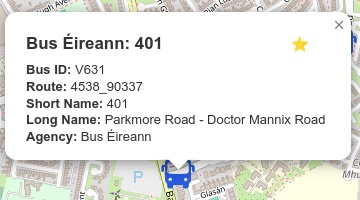
\includegraphics[width=\textwidth]{./images/favouritedbus.png}
        \caption{Bus pop-up with bus ``favourited''}
    \end{subfigure}
    \hfill
    \begin{subfigure}[c]{0.6\textwidth}
        \centering
        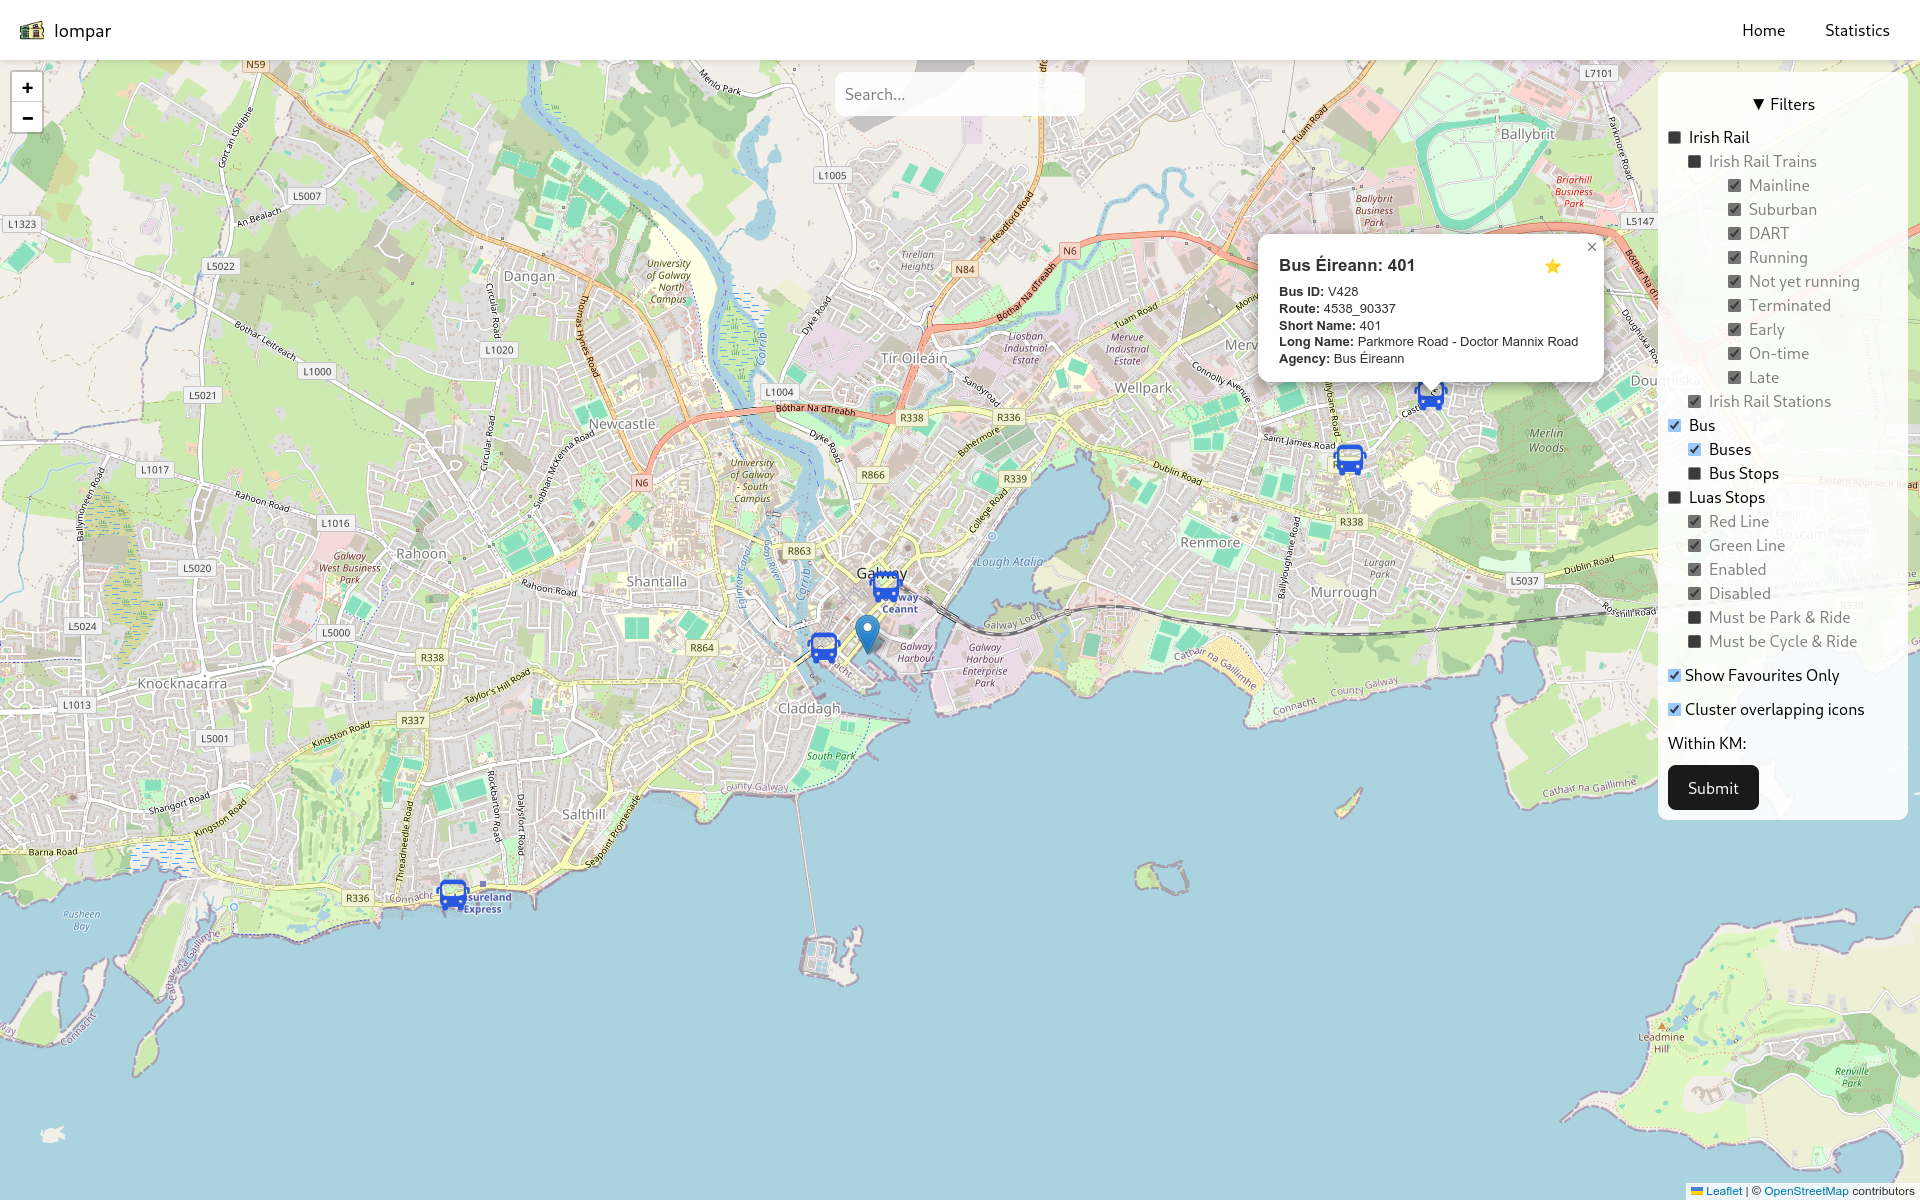
\includegraphics[width=\textwidth]{./images/401busesfavourited.png}
        \caption{Buses of the same route appearing when ``favourites only'' filter applied}
    \end{subfigure}
    \caption{Demonstration of the ``favourite'' functionality with buses}
\end{figure}

Train station pop-ups \& Luas stop pop-ups also have an additional button which, when clicked, fetches data about the services relating to that station.
This is necessary for Luas stops, as Luas data is only available on a per station basis, and just an extra feature for train stations, as train data is plotted on the map regardless.
The ``Load inbound/outbound trams'' button on the Luas stop pop-up fetches data from the \verb|/return_luas_data| API endpoint which contains the inbound and outbound trams due into that stop.
The ``Load incoming trains'' button on the train station pop-up fetches data from the \verb|/return_station_data| API endpoint which contains the trains due into that station in the next 90 minutes.
This information is then displayed in the pop-up itself, with a scrollbar if the information is too long to display in the pop-up without it becoming unmanageably long.

\begin{figure}[H]
    \centering
    \begin{subfigure}[c]{0.45\textwidth}
        \centering
        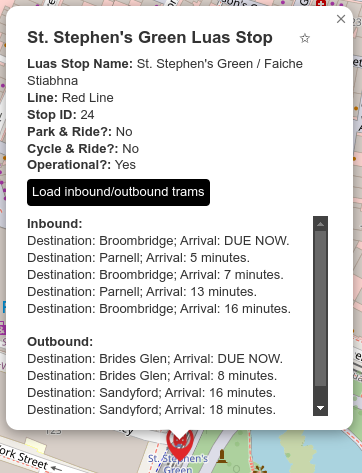
\includegraphics[width=\textwidth]{./images/loadinboundoutbound.png}
        \caption{Results of clicking ``Load inbound/outbound trams''}
    \end{subfigure}
    \hfill
    \begin{subfigure}[c]{0.38\textwidth}
        \centering
        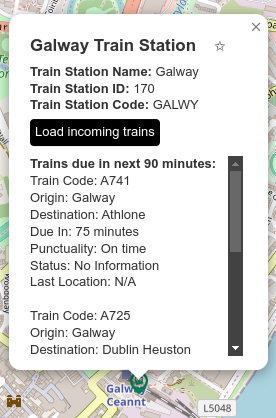
\includegraphics[width=\textwidth]{./images/loadstationdata.png}
        \caption{Results of clicking ``Load incoming trains''}
    \end{subfigure}
    \caption{Demonstration of the ``favourite'' functionality with buses}
\end{figure}

\subsubsection{Filters Side-Panel}
\begin{figure}[H]
    \centering
    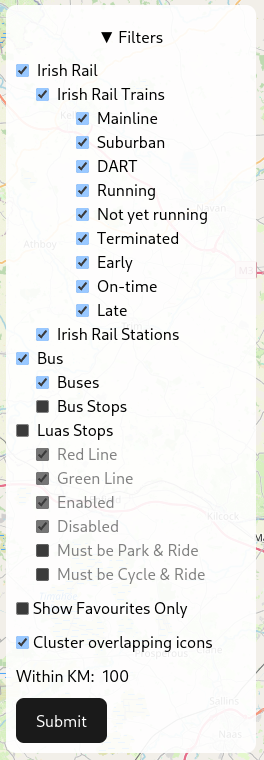
\includegraphics[width=0.3\textwidth]{./images/filterspanel.png}
    \caption{Screenshot of the filters side-panel}
\end{figure}

The Boolean filter variables mentioned in the display formulae above are selected by the user in the filters side-panel, implemented as a separate (presentational) component.
The component appears in the top-right hand corner of the screen, and can be minimised while browsing the map.
When a user clicks ``Submit'', the \mintinline{js}{fetchData()} function is invoked with the selected filters, and these selected filters are saved as a cookie to the user's browser; 
this cookie is loaded when the main page is first loaded, so that a user's last used filters are pre-selected for them when they open the application.
Even the value of the ``Within KM'' number is stored as a cookie and loaded in with page load so that a user's experience is a seamless as possible between uses.
\\\\
The first three top-level filters determine what data sources are used: Irish Rail, Bus, and/or Luas Stops.
If a top-level or second-level filter is deselected, all its child filters are greyed out and cannot be interacted with until all its parents are selected. 
By default, if no cookie is stored for a user, the top-level filters are all deselected and all of their children are selected, making it as easy as possible for the user to select what they want to filter by.
The only exception to this are the ``Must be Park \& Ride'' and the ``Must be Cycle \& Ride'' filters underneath ``Luas Stops'': these filters are more restrictive, and hide any item that does not match them, and so are not selected by default.
\\\\
The ``Cluster overlapping icons'' option does not change what data is shown, but how it is shown;
by default, any items whose icons overlap one another's at the current zoom level are \textit{clustered} into a single icon that displays the number of items which are contained within it using a Leaflet plug-in called \verb|Leaflet.markercluster|\supercite{leaflet_markercluster}.
This option toggles this behaviour, which may be desirable depending on the user's preferences, especially when only few items are being displayed in a small geographical area. 

\begin{figure}[H]
    \centering
    \begin{subfigure}[c]{0.49\textwidth}
        \centering
        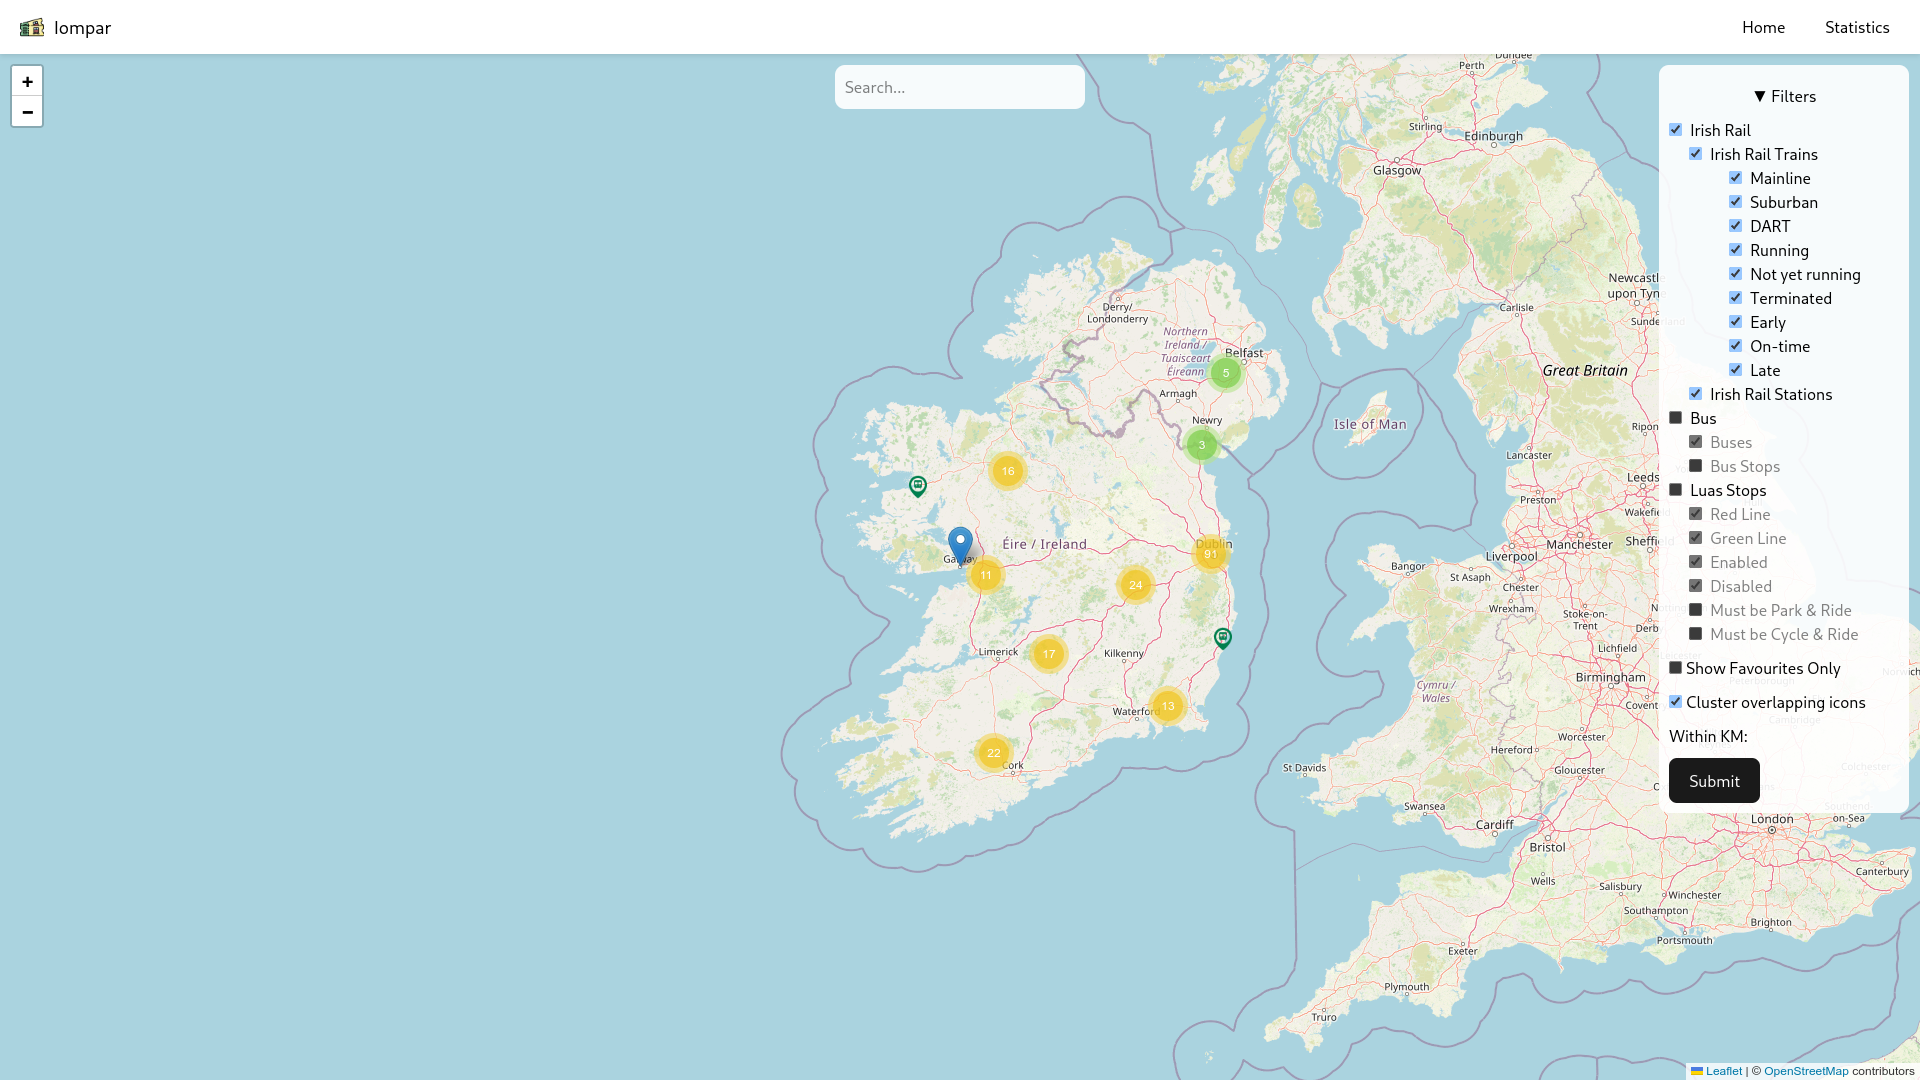
\includegraphics[width=\textwidth]{./images/clusteringenabled.png}
        \caption{Screenshot of the effects of enabling clustering}
    \end{subfigure}
    \hfill
    \begin{subfigure}[c]{0.49\textwidth}
        \centering
        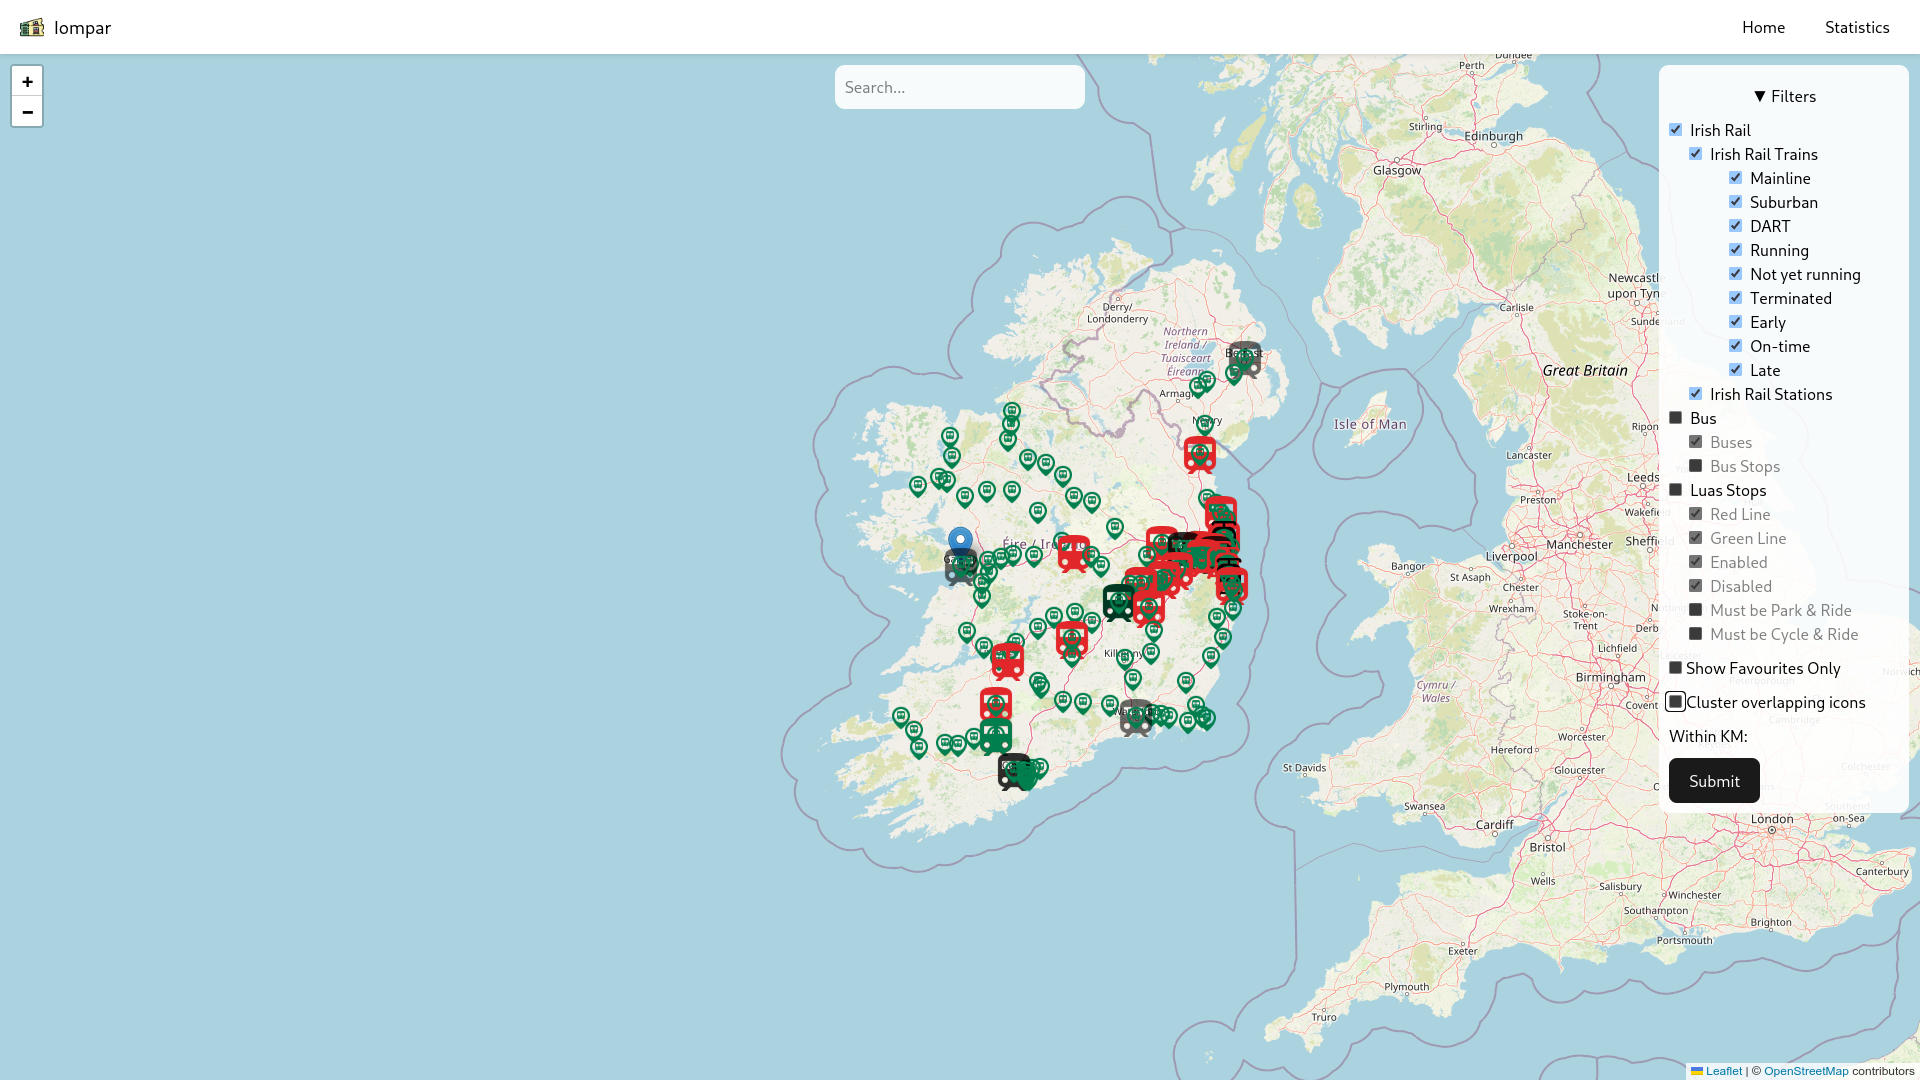
\includegraphics[width=\textwidth]{./images/clusteringdisabled.png}
        \caption{Screenshot of the effects of disabling clustering}
    \end{subfigure}
    \caption{Effects of enabling/disabling clustering}
\end{figure}

The ``Within KM'' option accepts a number input value of the range within which an item must be for it to be displayed.
This option only appears if the user's geographical location is available: if their browser does not support the option, or if they have rejected location access to the application, the option will not appear.
The option can be reset to showing all items regardless of range by deleting the input to the textbox;
if the user enters a value that doesn't make sense, such as a number $\leq$ 0, the application defaults to displaying all items regardless of distance, on the assumption that the user is either attempting to reset the filter by entering ``0'' or that they have accidentally entered a nonsensical value.
\\\\
A subject of much deliberation in the design process was the behaviour of the ``Submit'' button.
It's important that the map only updates when the user asks it to so as to avoid situations where the user is looking at an item, the page refreshes automatically, and it disappears from view;
therefore, fetching new data had to be a manually-specified process, rather than occurring automatically.
The question of whether or not the filters should be applied as soon as they are selected or only upon a ``Submit'' also received much consideration:
automatically updating them would minimise the amount of user interactions necessary, but to re-calculate the display value for every item when there are many being displayed could take a few seconds, and make the application unresponsive as the user makes many changes to the selected filters.
Therefore, it was decided that the filters should only be applied when the user requests that they be applied, so that they can decide what filters to apply in a convenient \& usable way.
Finally, there was the question of optimisations:
if the data sources selected did not change but a display filter did (for example, the user didn't change that they wanted to look at Irish Rail Trains, but added a selection to specify only Mainline trains), should another request be made to the API endpoints?
Not requesting new data would mean a faster loading time and a more responsive program, at the cost of showing the user potentially out-of-date data.
It was decided that each new click of ``Submit'' should always fetch new data, to align the program as much as possible with the user's mental model of the program, in keeping with the HCI principle of \textbf{conceptual model alignment}\supercite{norman_design_2013}: the behaviour of the application should match how the user imagines it to behave.
Users are familiar with the ``make selections, then confirm'' paradigm, and will expect the submit button to do the same thing each time (which aligns with Nielsen's usability heuristic of ``Consistency \& Standards'' and of ``speaking the user's language''\supercite{nielsenheuristics}).

\subsubsection{Search Bar}
The search bar allows the user to further refine the displayed items beyond what is possible with the filters side-panel by specifying text that should be present in the marker.
The search is based upon a \verb|markerText| variable that is constructed for each marker as the data is fetched, consisting of the pop-up content without any formatting, upper-case characters, or non-alphanumeric characters.
Similarly, entered search terms are made lower-case and stripped of non-alphanumeric characters to facilitate searching, and an item is deemed to match the search term if the search term occurs in the \verb|markerText|.
This approach is relatively simplistic as search algorithms go, but is fast \& efficient, and more than suitable for this application.

\begin{figure}[H]
    \centering
    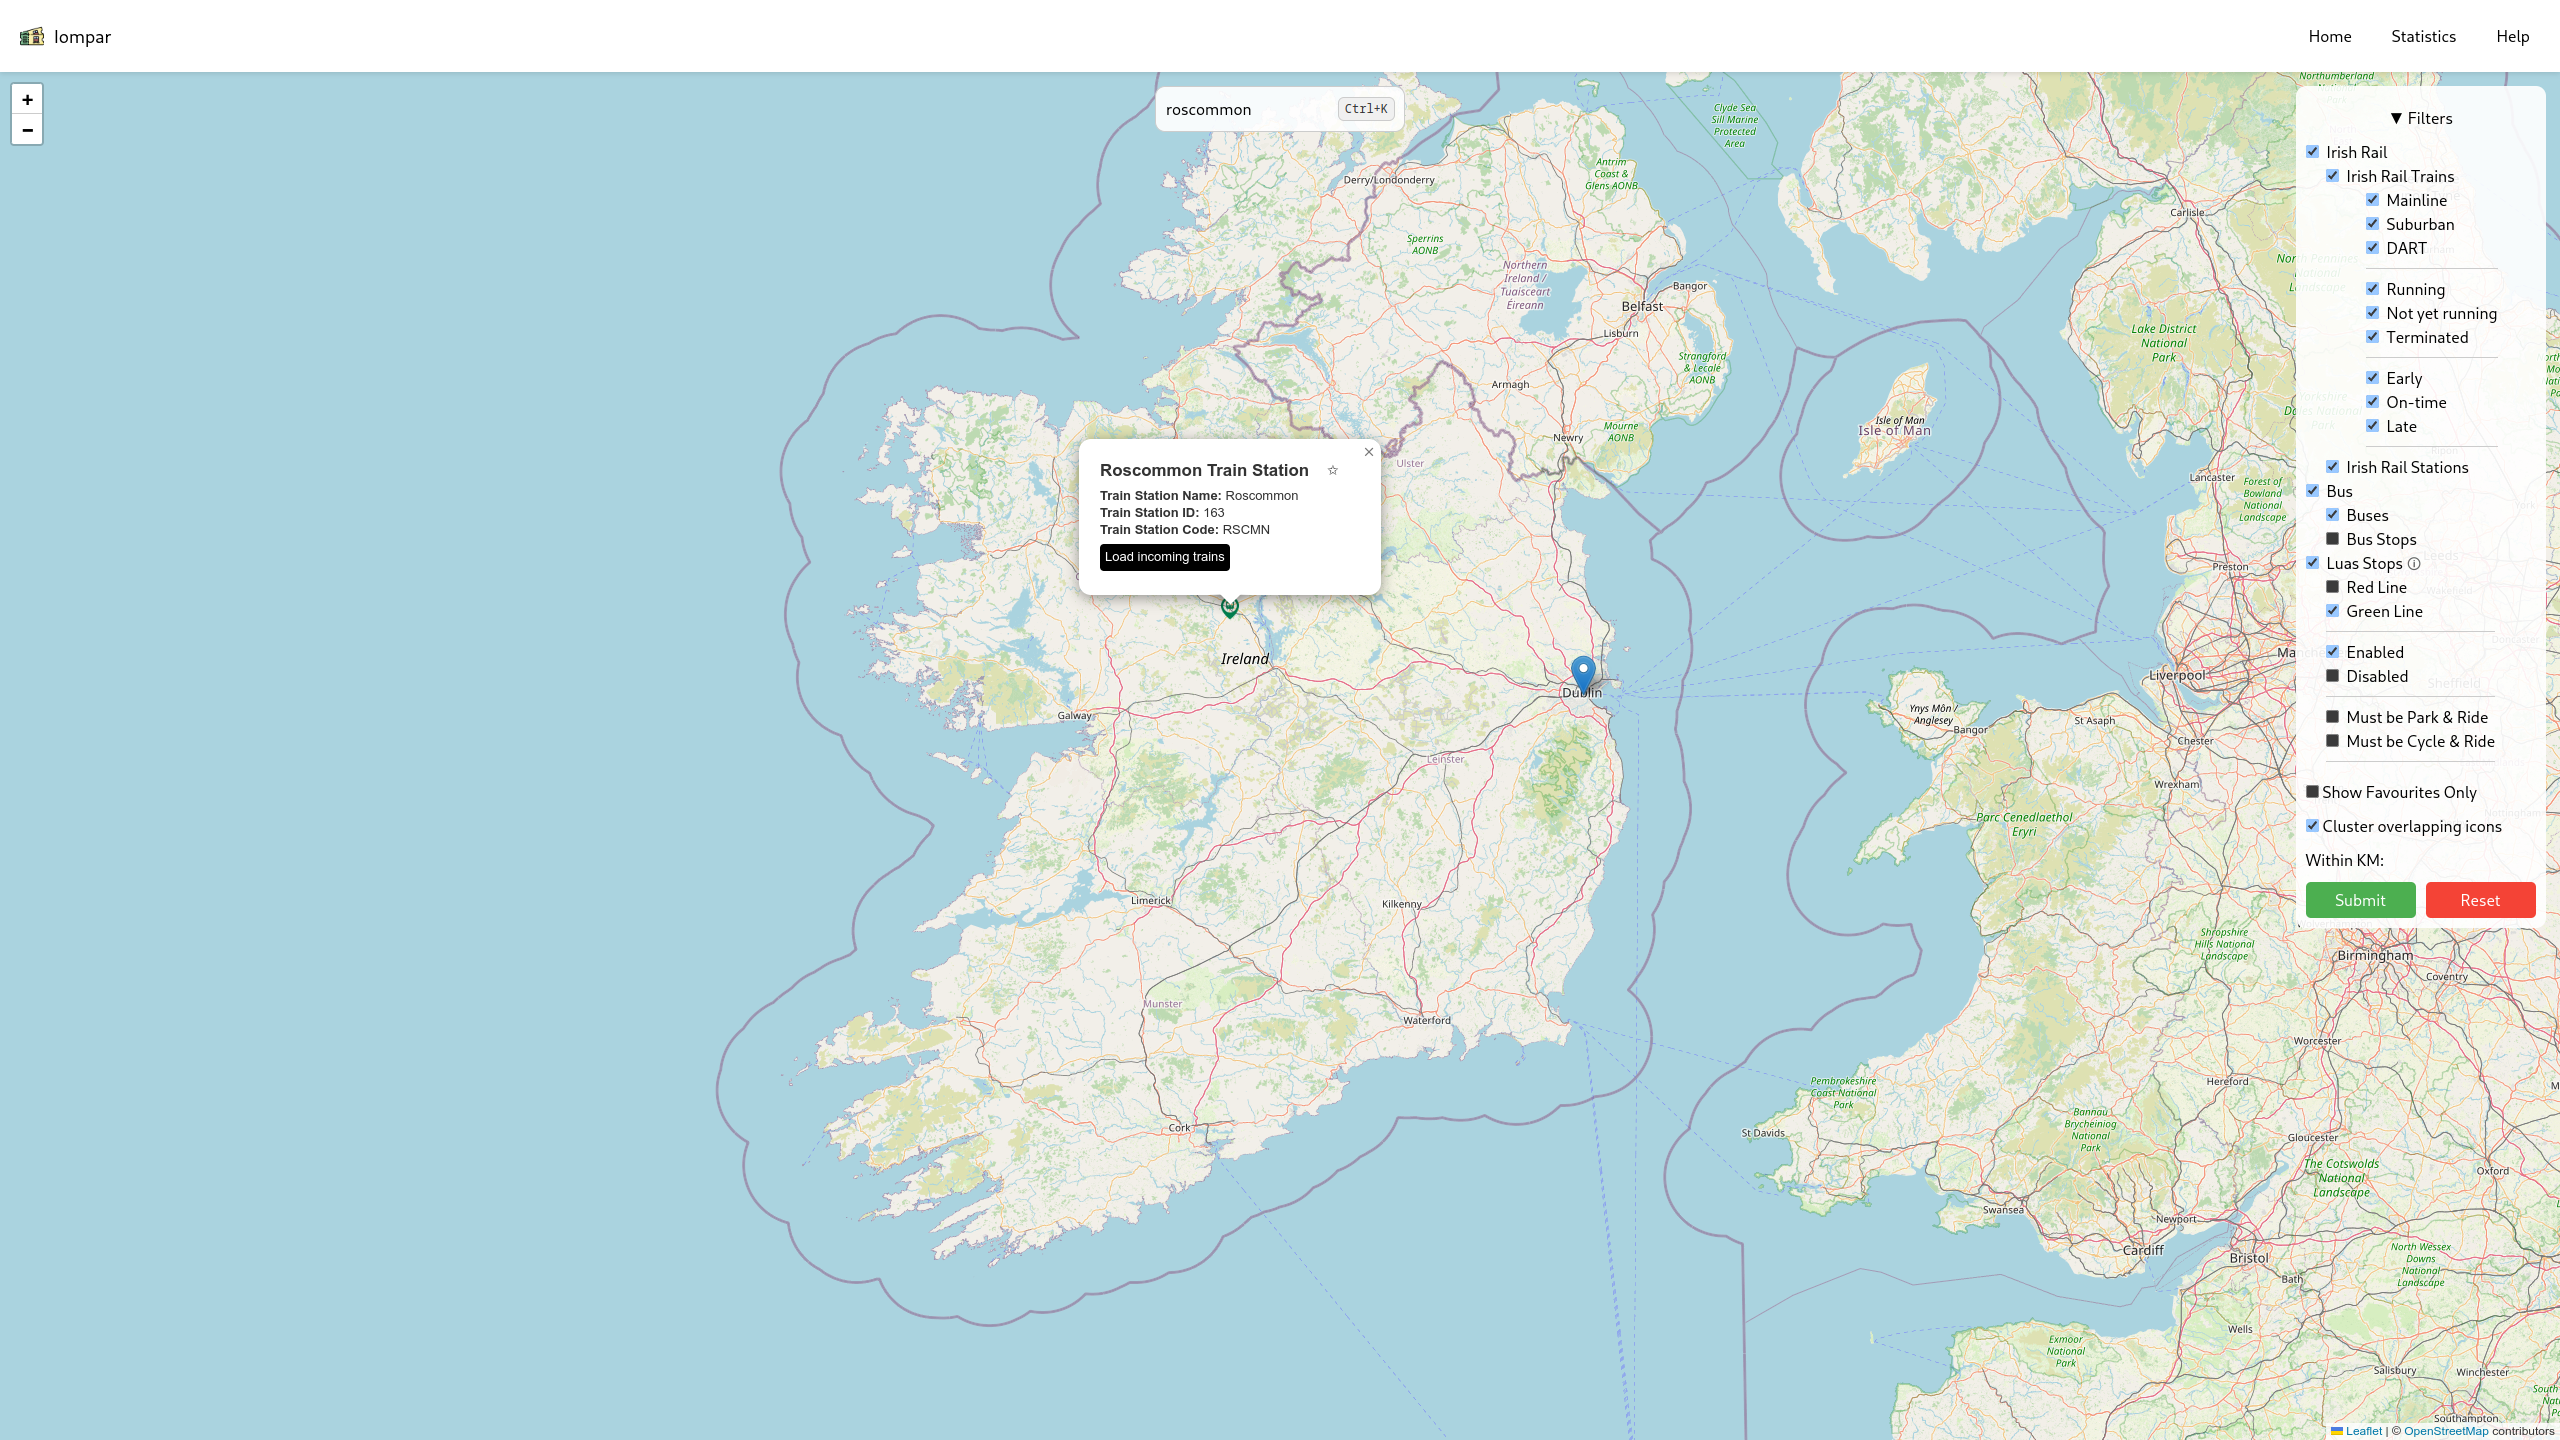
\includegraphics[width=\textwidth]{./images/searchstephens.png}
    \caption{Screenshot of the search bar being used}
\end{figure}

Unlike the filters panel, the displayed items are automatically filtered as the user enters text, which is facilitated by the search-based filtering being separated from and less computationally complex than the side-panel based filtering.
This allows the results to be quickly filtered in a responsive manner by the user, and makes the completion of tasks generally faster \& more responsive.
However, updating the filtered items for every keystroke that the user enters would be wasteful, as each key entry further refines their search and they would type it regardless, and constantly re-computing which items match the search term for each keypress would result in the application becoming less responsive.
To prevent this, the search bar employs a \textbf{debounce function}\supercite{debounce} which waits for a very short interval after the user's last keypress to start searching for the entered text;
the search will only commence once the user has finished typing.
Experiments with different values on different users indicated that 300 milliseconds is the ideal value for this application:
long enough that it won't be triggered until the user pauses typing, but short enough that the gap between the user stopping typing and the search being applied is nearly imperceptible.
\\\\
However, if very large amounts of data are being displayed, such as in the event that the user has selected all data sources, the search can take a noticeable amount of time and make the UI sluggish \& unresponsive as the search is executed.
To address this, if the number of items being displayed is so high that it will induce noticeably slow loading times, the debounce time is increased to 400 milliseconds to be more careful in avoiding unnecessary computations, and the loading overlay is displayed as the filtering is performed to prevent the user from being exposed to a sub-optimally performant UI.
\\\\
The search function makes use of the \mintinline{js}{useMemo}\supercite{usememo} React hook to cache the results of filtering the markers based off the search text, and making it so that it will only be re-calculated if the search term changes or if the markers change.
Without \mintinline{js}{useMemo}, every re-render of the page would cause the filter function to run even if nothing had changed, which would be a huge waste of computational resources.
\subsubsection{Map}
The map component itself is the presentational component in which all of the mapping \& plotting functionality is performed, implemented using the Leaflet\supercite{leaflet} mapping library and map tiles from OpenStreetMap\supercite{osm};
this option was chosen as it is lightweight \& performant, free to use, and is flexible \& customisable.
It is also by far the most popular mapping library, and has comprehensive documentation and a wide range of plug-ins.
Other mapping options exist, such as Mapbox\supercite{mapbox} and the Google Maps API\supercite{gmaps}, but these have limited free tiers compared to the completely free \& open-source option of Leaflet with OpenStreetMap.
It receives the markers to be displayed, a Boolean determining whether clustering is enabled, and the geolocation of the user, if available.
If the user's geolocation is available, a ``You are here'' marker is added to the map and the map is centered on those co-ordinates;
otherwise, the map centers on the geographical centre of the island of Ireland\supercite{osi} and displays no marker.
\\\\
Each marker variable component passed to the map component is added to the map, and if clustering is enabled, is wrapped in a \mintinline{js}{MarkerClusterGroup} to cluster the icons together if they overlap.

\section{Statistics Page}
\begin{figure}[H]
    \centering
    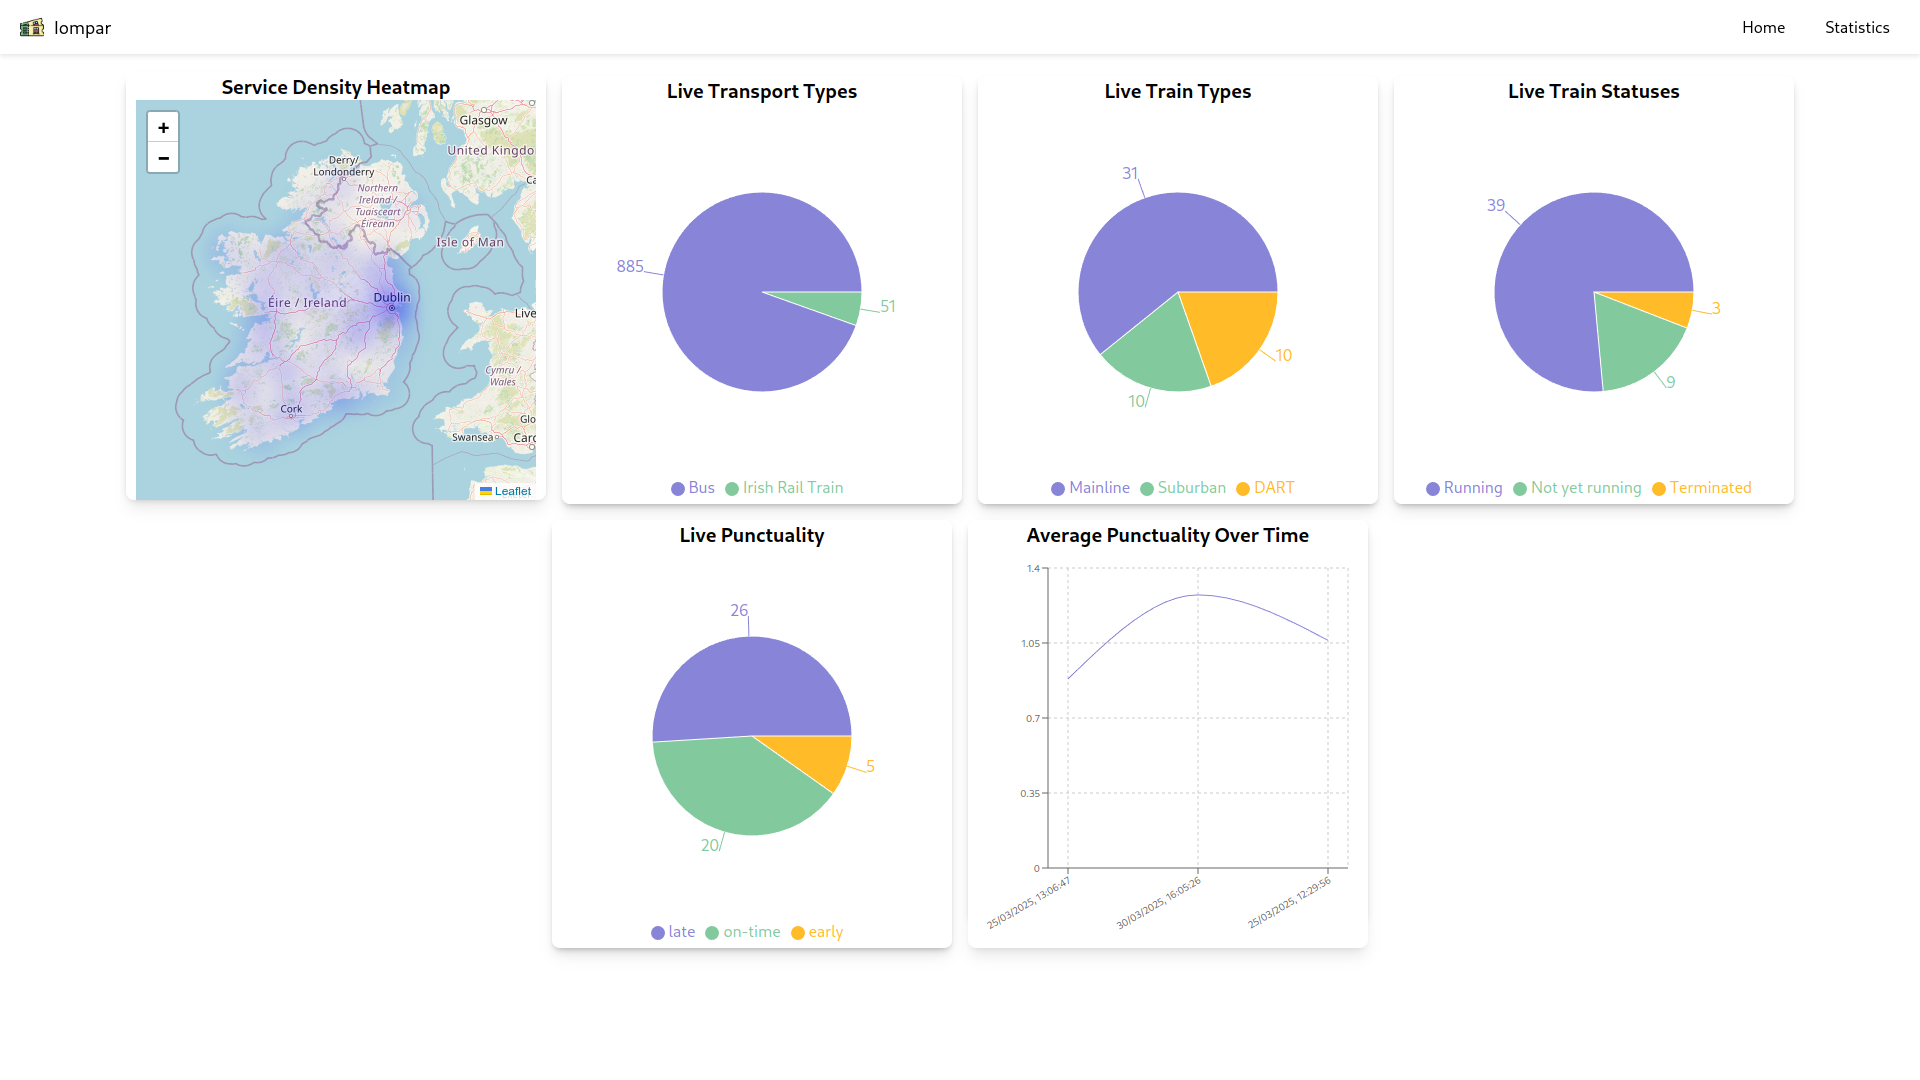
\includegraphics[width=\textwidth]{./images/statisiticspage.png}
    \caption{Screenshot of the statistics page}
\end{figure}

The statistics page of the application exists to give the user a deeper insight into the data than simply live data.
The grid layout is achieved with the use of Tailwind CSS flexbox\supercite{flexbox}.
It consists of 6 graphs, each displaying a different statistical insight about the application data:
\begin{itemize}
  \item   The Service Density Heatmap displays a heatmap depicting the geographical distribution of currently-running public transport services on the island of Ireland;
  \item   The Live Transport Types pie chart displays the proportion of \verb|objectType|s for which there is currently live location data;  
  \item The Live Train Types pie chart displays the proportion of mainline, suburban, \& DART Irish Rail Trains currently in operation;
  \item   The Live Train Statuses pie chart displays the proportion of running, not yet running, \& terminated trains at the present moment;
  \item   The Live Punctuality pie chart displays the proportion of late, on-time, \& early services at the present moment.
  \item   The Average Punctuality Over Time line graph displays how the average punctuality of services varies per collected \verb|timestamp|.
\end{itemize}

Each pie chart uses the same re-usable presentation component which accepts some data and displays it.
Pie charts are somewhat controversial in the realm of data visualisation and are often rejected in favour of bar charts, and are only recommended to be used under certain particular situations:
when the data being illustrated is a part-to-whole representation, when there is no more than 5 categories in the pie chart, and when there are not small differences between the categories\supercite{atlassianpiechart, spotfirepie, inforirver}.
Since the data for this application fulfils these criteria, and because testing with bar charts resulted with more difficult to understand results (as part of the proportion), pie charts were deemed suitable for this purpose.

\section{Help Page}
\begin{figure}[H]
    \centering
    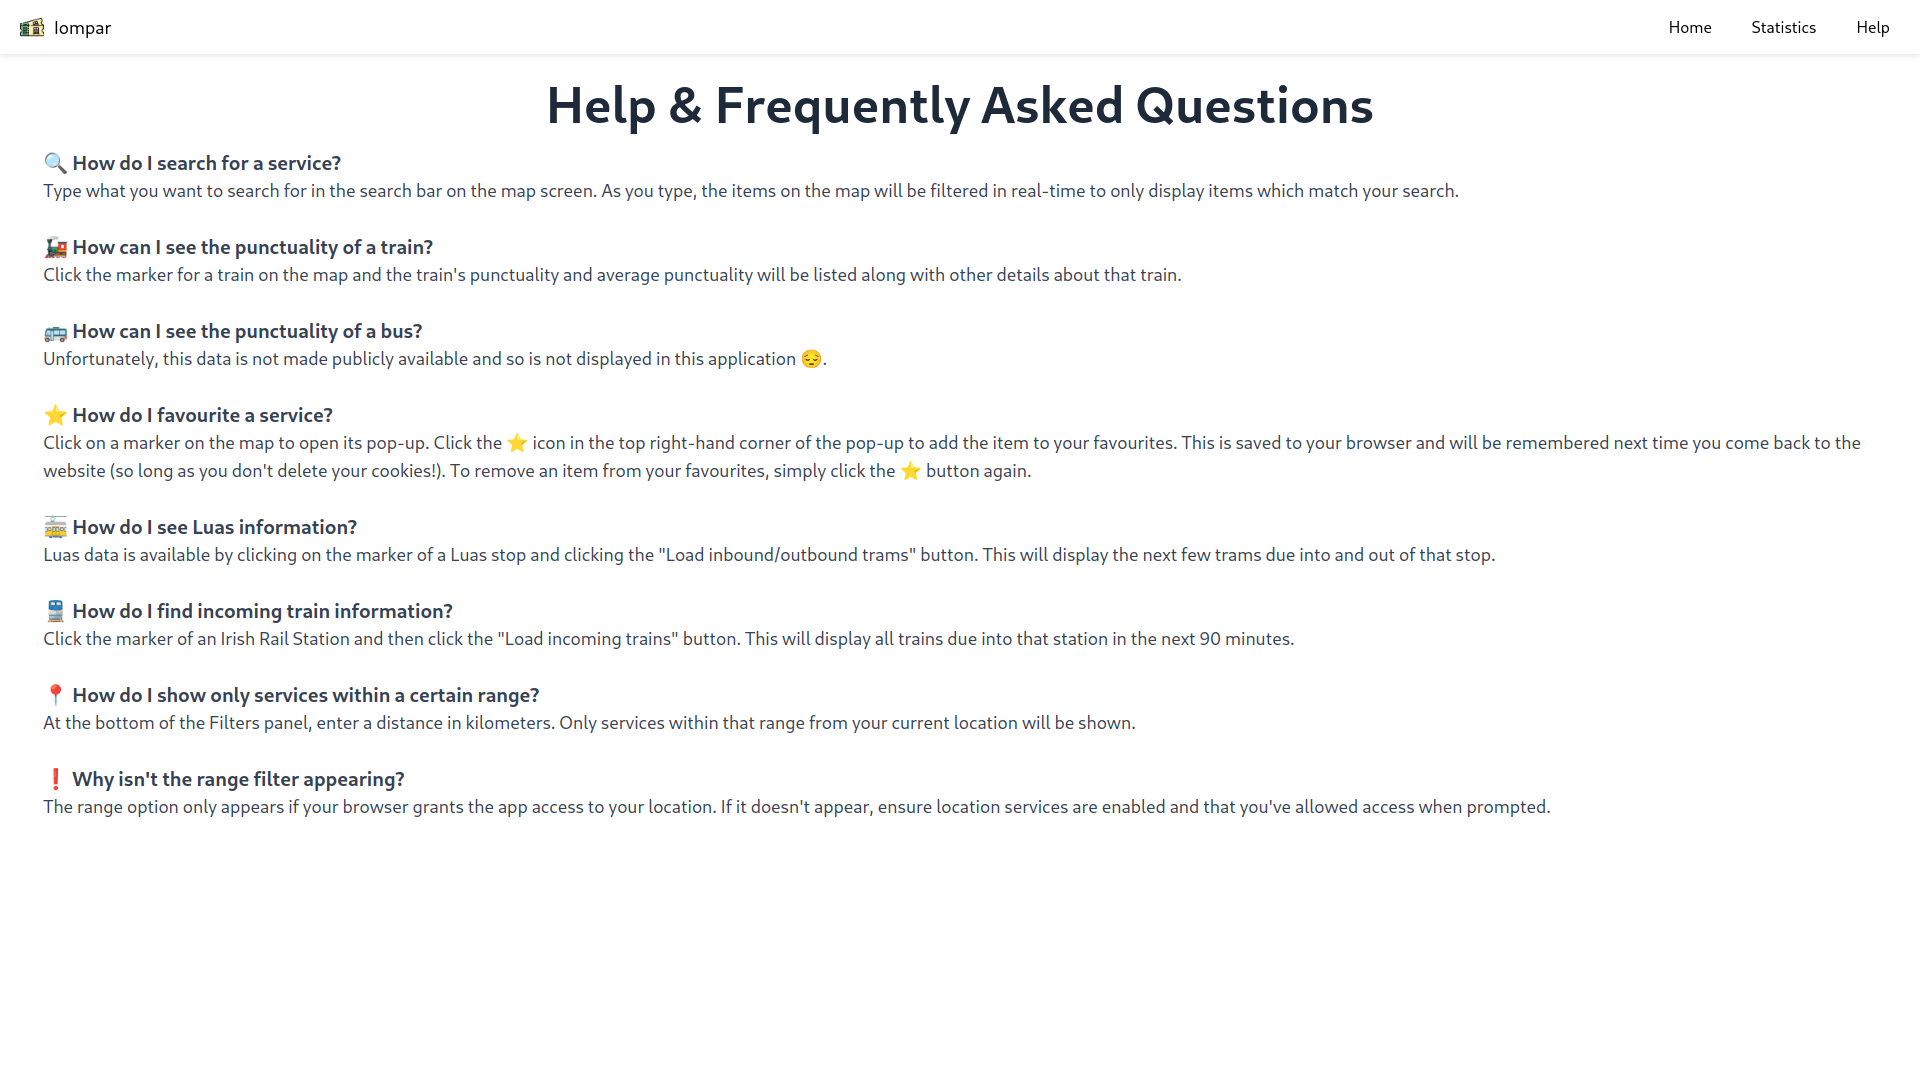
\includegraphics[width=\textwidth]{./images/helppage.png}
    \caption{Screenshot of the help page}
\end{figure}

The help page is a very simple web page that just contains questions and answers on how to perform basic tasks, such as favouriting an item or viewing real-time Luas information.
It is intended to be user-friendly and easy to search through; 
this is in part facilitated through its minimalist design (achieved with TailwindCSS) which attempts to prevent the user from having to sift through irrelevant information to find out how to perform a basic task.

\chapter{Evaluation}
\section{Objectives Completed}
Each of the core objectives set out for this project were completed:
\begin{enumerate}
    \item   A live map of train, DART, bus, \& Luas services in Ireland was created which displays the real-time whereabouts about the service, relevant information about that particular service, and the punctuality of the service, to the extent that is possible with publicly-available data.

    \item   The live map was given a powerful search tool which facilitates easy navigation \& use, such as allowing the user to find the particular service in which they are interested.

    \item   A side-panel was created with an extensive array of filters that can be applied to the map to limit what services are displayed, including filtering by transport mode \& punctuality.

    \item   A historical database was created in which historical data about public transport services is collected, with the insights gained from the historical data being made available to the user via relevant predictions about the punctuality of a service based off its track record.

    \item   The interface is responsive and is equally functional on both desktop \& mobile devices.
\end{enumerate}

Many additional objectives beyond the core objectives were also completed:
\begin{enumerate}
    \item   The application does not just have vehicle-based information, but also route-based information, allowing users to search for a particular bus route or service.
    
    \item   A feature was created to allow the user to ``favourite'' or save specific services, such as a particular bus route or Luas stop.

    \item   Cookies were employed to recall a user's selected filters and favourited items when they re-visit the page.

    \item   The user's geographical location is obtained via their browser's API and plotted on the map, and this information is used to allow users to filter results by proximity to themselves by specifying a radius.

    \item   The UI design complies with Nielsen's 10 Usability Heuristics.

    \item   The frontend performance was optimised and tuned to increase the loading speed of the application by several seconds.

    \item   The backend was cost-optimised to stay within the limit's of the AWS free tier.


    \item   Unit tests were written for each piece of backend code, with a line coverage of 85\% achieved, exceeding the minimum target value. 

    \item   A CI/CD pipeline was created which automatically tests and deploys new code.
\end{enumerate}

However, not all of the secondary objectives which were set out at the beginning of the project were completed:
\begin{enumerate}
    \item   No user account feature was added.
            The primary reason for this was just that it was quite low on the list of priorities, and so time wasn't made for it before the project deadline, although research was done into how it could be executed, and it likely would not be overly difficult.
            \textbf{Amazon Cognito}\supercite{cognito} provides a user directory, authentication server, and authorisation service, and therefore circumvents the need to create a sign-up process for the application and secure the database from scratch.
            It integrates into React with the \mintinline{js}{aws-amplify} library\supercite{amplify} which comes with a pre-built login/sign-up UI, and so practically no work would need to be completed to add an accounts system to the application: just enable the service and add some boilerplate React code.
            The only aspect that would require any substantial development effort would be the creation of a DynamoDB table with the primary key being the user's Cognito ID which stores the user's filters preferences;
            since these are already stored in JSON format on the user's machine, the structure would not have to be changed at all to add the information to the No-SQL database, and all that would need to be done would be to add a method for uploading the data.

    \item   No user review capability was added to allow users to report issues such as anti-social behaviour.
            This is primarily because of this feature being very low priority, and being dependent on the creation of a user account feature first to work;
            theoretically, a review system could be implemented without a user account system by just allowing anyone to \verb|POST| some data to an API which adds it to a database and displays it on the website, but this would be a very bad idea in practice both from a security point of view and from a spam \& vandalism prevention point of view.
            However, some research and planning was nonetheless carried out:
            a new DynamoDB table could be created with an item's \verb|objectID| as its partition key, and \verb|userID#timestamp| as the sort key, where \verb|userID| is the Cogito ID of the logged-in user and the \verb|timestamp| is the time the review was made.
            A form could be added to the frontend which uses \verb|aws-amplify| to make authorised \verb|POST| requests to an API endpoint.
            Then, when a user loads information about a given service, this table could be queried to display relevant user feedback about that service.
            In practice, there would need to be some kind of moderation of this review system to prevent spam, vandalism, \& to remove unhelpful reviews.

    \item   The web application was not made available online with a dedicated domain name.
            The first reason for this is simply to avoid the cost of acquiring a dedicated domain name, but the site could be made available online using an AWS S3 bucket\supercite{s3} (essentially serverless flat file storage) to store the website's build files, and accessed using the auto-generated S3 static endpoint URL;
            the second reason is that this would expose the application more fully to the open Internet, which could increase the number of API calls made, Lambda functions triggered, and risk pushing the application out of the free tier, although the risk of this is really quite low.
            The third and primary reason why this was not implemented is that its low priority led it to being sidelined in favour of more mission-critical work.

    \item   The React application was not ported to React native to run natively on Android \& iOS devices, nor was it published to relevant software distribution programs.
            In retrospect, this was a wildly over-optimistic goal to even consider for this project:
            while React Native greatly simplifies mobile application development, it is not a magic solution that completely removes the need for platform-specific development, and Android \& iOS knowledge would almost certainly be needed for debugging platform-specific issues or to utilise any native modules that don't have a React Native wrapper.
            Moreover, such development would require a development \& testing environment using Xcode and Android Studio, and would in doing so require at least a basic understanding of the two operating systems.
            Porting a web application as substantial as this one to React Native is non-trivial, as there are quite significant differences between the two, and would in itself constitute several months of work.
\end{enumerate}

Overall, $\frac{14}{18} = 77.\dot{7} \%$ of the specified objectives were completed, including $100\%$ completion of the core objectives, and completion of the majority of the secondary objectives;
objectives that were not completed were nonetheless researched and planned.

\section{Heuristic Evaluation: Nielsen's 10}
Nielsen's 10 usability heuristics for user interface design are a commonly-applied evaluation framework used by UX professionals to identify common usability issues, and so the application was defined with these heuristics in mind.

\subsection{Visibility of System Status}
\begin{quote}
    \textit{The design should always keep users informed about what is going on, through appropriate feedback within a reasonable amount of time}
\end{quote}

\subsection{User Control \& Freedom}
\begin{quote}
    \textit{Users often perform actions by mistake. They need a clearly marked "emergency exit" to leave the unwanted action without having to go through an extended process.}
\end{quote}

\subsection{Consistency \& Standards}
\begin{quote}
    \textit{ Users should not have to wonder whether different words, situations, or actions mean the same thing. Follow platform and industry conventions. }
\end{quote}

\subsection{Error Prevention}
\begin{quote}
    \textit{ Good error messages are important, but the best designs carefully prevent problems from occurring in the first place. Either eliminate error-prone conditions, or check for them and present users with a confirmation option before they commit to the action. }
\end{quote}

\subsection{Recognition Rather than Recall}
\begin{quote}
    \textit{ Minimize the user's memory load by making elements, actions, and options visible. The user should not have to remember information from one part of the interface to another. Information required to use the design (e.g. field labels or menu items) should be visible or easily retrievable when needed. }
\end{quote}

\subsection{Flexibility \& Efficiency of Use}
\begin{quote}
    \textit{ Shortcuts — hidden from novice users — may speed up the interaction for the expert user so that the design can cater to both inexperienced and experienced users. Allow users to tailor frequent actions. }
\end{quote}

\subsection{Aesthetic \& Minimalist Design}
\begin{quote}
    \textit{ Interfaces should not contain information that is irrelevant or rarely needed. Every extra unit of information in an interface competes with the relevant units of information and diminishes their relative visibility. }
\end{quote}

\subsection{Help users Recognise, Diagnose, \& Recover from Errors}
\begin{quote}
    \textit{ Error messages should be expressed in plain language (no error codes), precisely indicate the problem, and constructively suggest a solution. }
\end{quote}

\subsection{Help \& Documentation}
\begin{quote}
    \textit{ It’s best if the system doesn’t need any additional explanation. However, it may be necessary to provide documentation to help users understand how to complete their tasks. }
\end{quote}

\section{User Evaluation}

\chapter{Conclusion}









\printbibliography

\end{document}
